\chapter{Classical cluster algebras}
Mostly use \cite{FominWilliams2021IntroductionCA_1-3} as reference together with
Geoffrey's notes.

\section{Cluster algebras from quivers}

This first section serves as an introduction to cluster algebras. We will first look at
some examples of integer sequences arising from number theory or from combinatorial
data. In these examples, a few recurring observations will occur. These observations
will be explained by viewing each of the examples under the lens of cluster algebra
theory. We do not yet provide the most general definition of a cluster algebra, which
will instead be done in \cref{sec:ice_quivers_and_coefficients}. Instead, we focus on
the simplest case of a cluster algebra associated to a quiver. This case is easier to
grasp, and allows understanding the general concepts without getting distracted by
technical details.

\subsection{Combinatorial integer sequences}\label{sec:integer_sequences}

Let us start by looking at some integer sequences coming from number theory or
combinatorial data. Along the way we observe some interesting patterns which will be
explained by viewing these sequences as arising from a cluster algebra. \medskip

\begin{example}\label{exmp:markov_sequence}
	Consider the sequence given by the recurrence relation
	\begin{equation*}
		x_{n+3} = \frac{x_{n+1}^2 + x_{n+2}^2}{x_n},
	\end{equation*}
	with initial conditions $x_0 = x_1 = x_2 = 1$. Computing the first few terms gives
	\begin{equation*}
		1,1,1,2,5,29,433,37666,48928105,\dots
	\end{equation*}
	%
	Even though the recurrence relation involves a fraction, all the terms of the sequence
	are positive integers. We will explain this later, as a consequence of a more general
	fact about cluster algebras. Another way to observe this is as follows. For each $n \in
		\bbZ_{\geq0}$, the triple $(x_n, x_{n+1}, x_{n+2})$ satisfies the equation
	\begin{equation}\label{eq:markov_diophantine}
		x_n^2 + x_{n+1}^2 + x_{n+2}^2 = 3 x_n x_{n+1}x_{n+2},
	\end{equation}
	known as the \emph{Markov equation}\index{Markov!equation}\footnote{It is named after Andrey Markov. This is the same mathematician after whom Markov chains are named.}. The case $n = 0$ is clear. Then, by induction, we have
	\begin{equation}\label{eq:markov_mutation_simplified}
		x_{n+3} = \frac{x_{n+1}^2 + x_{n+2}^2}{x_n} = \frac{3 x_n x_{n+1}x_{n+2} - x_n^2}{x_n} = 3 x_{n+1} x_{n+2} - x_n,
	\end{equation}
	so that
	\begin{align*}
		x_{n+3}^2 + x_{n+2}^2 + x_{n+1}^2
		 & = (3 x_{n+1}x_{n+2} - x_n)^2 + x_{n+1}^2 + x_{n+2}^2                            \\
		 & = 9 x_{n+1}^2 x_{n+2}^2 - 6 x_{n+1} x_{n+2} x_n + x_n^2 + x_{n+1}^2 + x_{n+2}^2 \\
		 & = 9 x_{n+1}^2 x_{n+2}^2 - 6 x_n x_{n+1} x_{n+2} + 3 x_n x_{n+1} x_{n+2}         \\
		 & = 9 x_{n+1}^2 x_{n+2}^2 - 3 x_n x_{n+1} x_{n+2}                                 \\
		 & = 3 ( x_{n+1} x_{n+2}-  x_n) x_{n+1} x_{n+2}                                    \\
		 & = 3 x_{n+3} x_{n+1} x_{n+2}.
	\end{align*}
	%
	The intermediate result, \cref{eq:markov_mutation_simplified}, also immediately implies
	that all the terms in the sequence are integers. That they are positive follows from
	the recurrence relation itself.
\end{example}

\begin{example}\label{exmp:somos4}

	Let $a_n$ be the sequence defined through the recurrence relation
	\begin{equation}
		\label{eq:somos_4}
		a_{n+4} = \frac{a_{n+3}a_{n+1}+ a_{n+2}^2}{a_n}
	\end{equation}
	%
	with initial conditions $a_0 = a_1 = a_2 = a_3 = 1$. This sequence is known as the
	\emph{Somos-4}\index{Somos-4 sequence} sequence, named after its inventor, Michael
	Somos. It can be seen as a slight generalization of the sequence from
	\cref{exmp:markov_sequence}. Computing the first few terms of the sequence, we find:
	\begin{align*}
		 & \begin{aligned}
			   a_4 & = \frac{1 \cdot 1 + 1^2}{1} = 2                   \\
			   a_5 & = \frac{2 \cdot 1 + 1^2}{1} = 3                   \\
			   a_6 & = \frac{3 \cdot 1 + 2^2}{1} = 7                   \\
			   a_7 & = \frac{7 \cdot 2 + 3^2}{2} = 23                  \\
			   a_8 & = \frac{23 \cdot 3 + 7^2}{2} = \frac{118}{2} = 59 \\
		   \end{aligned}
		 &
		\begin{aligned}
			a_9    & = \frac{59 \cdot 7 + 23^2}{3} = \frac{942}{3} = 314                       \\
			a_{10} & = \frac{314 \cdot 23 + 59^2}{7} = \frac{10703}{7} = 1529                  \\
			a_{11} & = \frac{1529 \cdot 59 + 314^2}{23} = \frac{188807}{23} = 8209             \\
			a_{12} & = \frac{8209 \cdot 314 + 1529^2}{59} = \frac{4915467}{59} = 83313         \\
			a_{13} & = \frac{83313 \cdot 1529 + 8209^2}{314} = \frac{194773258}{314} = 620297.
		\end{aligned}
	\end{align*}
	%
	Just like in the previous example, there is no reason, a priori, to assume that all the
	elements of the sequence would be integers. However, somewhat remarkably, the
	denominators seem to always cancel out perfectly. Viewing this sequence through the
	cluster algebra framework, it will follow immediately that all the terms are indeed
	integers, as a corollary of the \emph{Laurent phenomenon}\index{Laurent!-phenomenon}.
\end{example}

\begin{example}\label{exmp:frieze_patterns}

	The next family of integer sequences comes from \emph{$\SL_2(\bbZ)$-frieze
		patterns}\footnote{The name ``frieze pattern'' comes from architecture, where it refers
		to a horizontal strip, often found just below the roofline, which is decorated with
		patterns.}\index{frieze pattern}\index{SL 2 Z@$\SL_2(\bbZ)$}. The idea of a frieze
	pattern is best explained through an example (\cite{Coxeter1971FriezePatterns}). Take
	for example the following pattern:
	\begin{equation*}
		\dots\quad
		\begin{tikzcd}[
				sep = 0.2em, cramped,
			]
			&0&&0&&0&&0&&0&&0&&0&&0&&0&&0&&0\\
			1&&1&&1&&1&&1&&1&&1&&1&&1&&1&&1\\
			&1&&2&&2&&3&&1&&2&&4&&1&&2&&2&&3\\
			3&&1&&3&&5&&2&&1&&7&&3&&1&&3&&5\\
			&2&&1&&7&&3&&1&&3&&5&&2&&1&&7&&3\\
			3&&1&&2&&4&&1&&2&&2&&3&&1&&2&&4\\
			&1&&1&&1&&1&&1&&1&&1&&1&&1&&1&&1\\
			0&&0&&0&&0&&0&&0&&0&&0&&0&&0&&0
		\end{tikzcd}
		\quad
		\dots
	\end{equation*}
	The defining property is that the $2 \times 2$ diamonds
	\begin{equation*}
		\begin{matrix}
			  & b &   \\
			a &   & d \\
			  & c &
		\end{matrix}
	\end{equation*}
	formed by adjacent elements, can be seen as an element of $\SL_2 (\bbZ)$, i.e., $ad - bc = 1$. Other than the bounding rows of ones and zeros, there is no additional requirement. In what follows we will omit the irrelevant row of zeros.

	One could ask if it is always possible to construct such a pattern for any number of
	rows. If so, one might be interested in knowing how many such patterns there are.
	Furthermore, one might notice that the pattern is periodic, repeating every 7 columns.
	In fact, the pattern even has ``half-periodicity'' where the marked triangle undergoes
	a translation and reflection.
	\begin{equation*}
		\dots\quad
		\begin{tikzcd}[
				sep = 0.2em, cramped,
				execute at end picture = {
						\draw[blue, dashed, rounded corners]
						($(\tikzcdmatrixname-1-1.north west) + (-0.3, 0.05)$) -- ($(\tikzcdmatrixname-1-11.north east)+ (0.3, 0.05)$)--($(\tikzcdmatrixname-6-6.south) + (0,-0.05)$) -- cycle;
						\draw[red, dashed, rounded corners]
						($(\tikzcdmatrixname-6-8.south west) + (-0.3, -0.05)$) -- ($(\tikzcdmatrixname-6-18.south east)+ (0.3, -0.05)$)--($(\tikzcdmatrixname-1-13.north) + (0,0.05)$) -- cycle;
					}
			]
			1&&1&&1&&1&&1&&1&&1&&1&&1&&1&&1\\
			&1&&2&&2&&3&&1&&2&&4&&1&&2&&2&&3\\
			3&&1&&3&&5&&2&&1&&7&&3&&1&&3&&5\\
			&2&&1&&7&&3&&1&&3&&5&&2&&1&&7&&3\\
			3&&1&&2&&4&&1&&2&&2&&3&&1&&2&&4\\
			&1&&1&&1&&1&&1&&1&&1&&1&&1&&1&&1\\
		\end{tikzcd}
		\quad
		\dots
	\end{equation*}

	To make such a pattern, we start with the observation that the rest of the pattern is
	completely determined by a lattice path from top to bottom. Indeed, using the
	$\SL_2(\bbZ)$ rule, one can fill in the rest of the pattern. For example, say we
	started with the following partially filled in pattern:
	\begin{equation*}
		\dots\quad
		\begin{tikzcd}[
				sep = 0.2em, cramped,
			]
			1&&1&&1&&1&&1&&1&&1\\
			&a\\
			b\\
			&1&&1&&1&&1&&1&&1\\
		\end{tikzcd}
		\quad
		\dots
	\end{equation*}
	then the rest has to be filled out as follows
	\begin{equation*}
		\dots\quad
		\begin{tikzcd}[
				sep = 0.2em, cramped,
			]
			1&&1&&1&&1&&1&&1&&1\\
			&a&& \frac{1+a+b}{ab} && b && \frac{1+a}{b} && \frac{1+b}{a} && a\\
			b&& \frac{1+a}{b} &&  \frac{1+b}{a} && a && \frac{1+a+b}{ab} && b\\
			&1&&1&&1&&1&&1&&1\\
		\end{tikzcd}
		\quad
		\dots
	\end{equation*}
	%
	Since all the denominators are monomials in $a$ and $b$, it follows that when $a = b =
		1$, all the elements will be integers, as required.

	It seems that we somehow got lucky in this case. There is again, a priori, no reason to
	assume that for any number of rows, we will always be able to choose the initial
	integers such that all the fractions simplify. The fact that this is possible, follows
	again from the ``Laurent phenomenon''\index{Laurent!-phenomenon}, on which we can now
	shed a bit more light. Let $a_1, a_2, \dots, a_n$ be the initial integers chosen on the
	lattice path. Then, in this context, the Laurent phenomenon states that all the other
	elements of the frieze pattern can be written as Laurent
	polynomials\index{Laurent!-polynomial} in $a_1 , \dots, a_n$ with coefficients in
	$\bbZ$, i.e., as an element of $\bbZ [a_1 ^\pm, \dots, a_n^\pm]$. So, any lattice path
	from top to bottom consisting of only ones, will yield a frieze pattern. This already
	proves the existence of such frieze patterns for any number of rows. We will return to
	the other questions in \cref{sec:sequences_revisited}.
\end{example}

The last example will be based on the following theorem from Euclidean geometry.
\begin{theorem}[Ptolomy's Theorem]\label{thm:ptolomy}

	Let $A,B,C,D$ be distinct points on a circle, in cyclic order (\cref{fig:ptolomy}).
	These determine vertices of a quadrilateral, where the side, and diagonal lengths
	satisfy the following rule:
	\begin{equation*}
		|AC| \cdot |BD| = |AB|\cdot |CD| + |AD| \cdot |BC|.
	\end{equation*}
\end{theorem}

\begin{figure}[ht!]
	\centering

	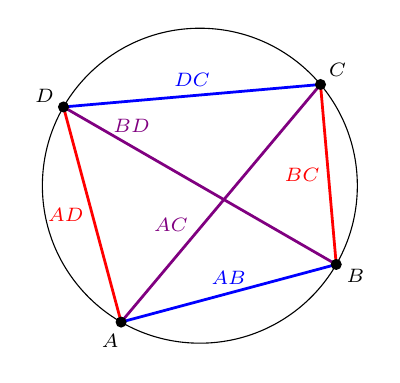
\begin{tikzpicture}
		\coordinate (center) at (0,0);
		\def\radius{2cm}
		\draw (center) circle[radius=\radius];

		% points on the circle
		\path (center) ++(-120:\radius) coordinate (A);
		\path (center) ++(-30:\radius) coordinate (B);
		\path (center) ++(40:\radius) coordinate (C);
		\path (center) ++(150:\radius) coordinate (D);

		\begin{scriptsize}
			% Chords
			\draw[color=red, line width=1pt] (A) -- node[left] {$AD$} (D);
			\draw[color=red, line width=1pt] (B) -- node[left] {$BC$} (C);
			\draw[color=blue, line width=1pt] (A) -- node[above] {$AB$} (B);
			\draw[color=blue, line width=1pt] (D) -- node[above] {$DC$} (C);
			\draw[color=violet, line width=1pt] (A) -- node[above=8pt, near start] {$AC$} (C);
			\draw[color=violet, line width=1pt] (D) -- node[above=2pt, near start] {$BD$} (B);

			% Draw the points over the chords
			\fill[black] (A) circle[radius=2pt] ++(-120:1em) node {$A$};
			\fill[black] (B) circle[radius=2pt] ++(-30:1em) node {$B$};
			\fill[black] (C) circle[radius=2pt] ++(40:1em) node {$C$};
			\fill[black] (D) circle[radius=2pt] ++(150:1em) node {$D$};

		\end{scriptsize}
	\end{tikzpicture}
	\caption{Ptolomy's theorem:
	${\color{violet} |AC| \cdot |BD|}
		= {\color{red} |AD|\cdot |BC|} + {\color{blue} |AB| \cdot |CD|}$.}
	\label{fig:ptolomy}
\end{figure}

\begin{example}\label{exmp:triangulations}

	Note that \cref{thm:ptolomy} allows one to compute the length of one of the diagonals
	in terms of the other, given the side lengths. We will now apply this to triangulations
	of polygons.

	Let $1, 2, \dots, n$ denote $n$ points on a circle, arranged in cyclic order. By
	connecting the points $i$ and $i +1$ for $i \in [1, n]$, where the indices are taken
	modulo $n$, we obtain a polygon with $n$ sides. A triangulation\index{triangulations!of
		polygons}, $T$, is a choice of $(n-3)$ non-crossing diagonals. This results in a
	partitioning of the polygon in $n-2$ triangles. We will see triangulations in much more
	detail in \cref{sec:triangulations_of_surfaces}, and will therefore keep things brief
	here. For now, it is enough to understand things visually (cf.
	\cref{fig:hexagon_triangulations}).
	\begin{figure}[ht]
		\centering

		\begin{tikzpicture}
			\node[name=h, shape=regular polygon, draw, regular polygon sides = 6, minimum size = 1.5cm]{};
			\draw[] (h.corner 1) -- (h.corner 3);
			\draw[] (h.corner 1) -- (h.corner 4);
			\draw[] (h.corner 1) -- (h.corner 5);
		\end{tikzpicture}
		\begin{tikzpicture}
			\node[name=h, shape=regular polygon, draw, regular polygon sides = 6, minimum size = 1.5cm]{};
			\draw[] (h.corner 2) -- (h.corner 5);
			\draw[] (h.corner 2) -- (h.corner 4);
			\draw[] (h.corner 1) -- (h.corner 5);
		\end{tikzpicture}
		\begin{tikzpicture}
			\node[name=h, shape=regular polygon, draw, regular polygon sides = 6, minimum size = 1.5cm]{};
			\draw[] (h.corner 1) -- (h.corner 3);
			\draw[] (h.corner 3) -- (h.corner 5);
			\draw[] (h.corner 1) -- (h.corner 5);
		\end{tikzpicture}
		\caption{The triangulations of a regular hexagon up to rotations and reflections.}
		\label{fig:hexagon_triangulations}
	\end{figure}

	Starting from a triangulation, $T$, we obtain a new triangulation, $T'$, by
	``flipping'' a diagonal. Any diagonal in a triangulation lies on precisely 2 triangles.
	These two triangles form a quadrilateral. To flip the diagonal, you replace it with the
	other diagonal of that quadrilateral. Again, this is most easily seen visually:
	\begin{equation*}
		\begin{tikzpicture}[baseline]
			\node[name=h, shape=regular polygon, draw, regular polygon sides = 6, minimum size = 1.5cm]{};
			\draw[] (h.corner 1) -- (h.corner 3);
			\draw[dashed] (h.corner 1) -- (h.corner 4);
			\draw[] (h.corner 1) -- (h.corner 5);
		\end{tikzpicture}
		\quad \leadsto \quad
		\begin{tikzpicture}[baseline]
			\node[name=h, shape=regular polygon, draw, regular polygon sides = 6, minimum size = 1.5cm]{};
			\draw[] (h.corner 1) -- (h.corner 3);
			\draw[dashed] (h.corner 3) -- (h.corner 5);
			\draw[] (h.corner 1) -- (h.corner 5);
		\end{tikzpicture}
	\end{equation*}

	Using Ptolomy's theorem, the length of the new diagonal can be computed given that we
	knew the lengths of all the edges in the previous triangulation. We now ignore
	Euclidean geometry, and just use Ptolomy's theorem as a recurrence relation to
	construct a collection of numbers as follows. Pick a triangulation and set all the edge
	lengths equal to one. Then, at each step, choose a diagonal in the triangulation and
	flip it. Compute its edge length using Ptolomy's theorem. This is the next number in
	the collection. For example, we could obtain a sequence starting like this (we omit the
	ones on the sides):
	\begin{equation*}
		\begin{tikzpicture}[baseline]
			\node[name=h, shape=regular polygon, draw, regular polygon sides = 6, minimum size = 1.5cm]{};
			\draw[] (h.corner 1) -- node[fill=white, font=\footnotesize] {1} (h.corner 3);
			\draw[] (h.corner 1) -- node[fill=white, font=\footnotesize] {1} (h.corner 4);
			\draw[] (h.corner 1) -- node[fill=white, font=\footnotesize] {1} (h.corner 5);
		\end{tikzpicture}
		\leadsto
		\begin{tikzpicture}[baseline]
			\node[name=h, shape=regular polygon, draw, regular polygon sides = 6, minimum size = 1.5cm]{};
			\draw[] (h.corner 1) -- node[fill=white, font=\footnotesize] {1} (h.corner 3);
			\draw[dashed] (h.corner 3) -- node[fill=white, font=\footnotesize] {2} (h.corner 5);
			\draw[] (h.corner 1) -- node[fill=white, font=\footnotesize] {1} (h.corner 5);
		\end{tikzpicture}
		\leadsto
		\begin{tikzpicture}[baseline]
			\node[name=h, shape=regular polygon, draw, regular polygon sides = 6, minimum size = 1.5cm]{};
			\draw[dashed] (h.corner 2) -- node[fill=white, font=\footnotesize] {3} (h.corner 5);
			\draw[] (h.corner 3) -- node[fill=white, font=\footnotesize] {2} (h.corner 5);
			\draw[] (h.corner 1) -- node[fill=white, font=\footnotesize] {1} (h.corner 5);
		\end{tikzpicture}
		\leadsto
		\begin{tikzpicture}[baseline]
			\node[name=h, shape=regular polygon, draw, regular polygon sides = 6, minimum size = 1.5cm]{};
			\draw[] (h.corner 2) -- node[fill=white, font=\footnotesize] {3} (h.corner 5);
			\draw[] (h.corner 3) -- node[fill=white, font=\footnotesize] {2} (h.corner 5);
			\draw[dashed] (h.corner 2) -- node[fill=white, font=\footnotesize] {4} (h.corner 6);
		\end{tikzpicture}
		\leadsto
		\begin{tikzpicture}[baseline]
			\node[name=h, shape=regular polygon, draw, regular polygon sides = 6, minimum size = 1.5cm]{};
			\draw[dashed] (h.corner 3) -- node[fill=white, font=\footnotesize] {3} (h.corner 6);
			\draw[] (h.corner 3) -- node[fill=white, font=\footnotesize] {2} (h.corner 5);
			\draw[] (h.corner 2) -- node[fill=white, font=\footnotesize] {4} (h.corner 6);
		\end{tikzpicture}
		\leadsto
		\begin{tikzpicture}[baseline]
			\node[name=h, shape=regular polygon, draw, regular polygon sides = 6, minimum size = 1.5cm]{};
			\draw[] (h.corner 3) -- node[fill=white, font=\footnotesize] {3} (h.corner 6);
			\draw[] (h.corner 3) -- node[fill=white, font=\footnotesize] {2} (h.corner 5);
			\draw[dashed] (h.corner 3) -- node[fill=white, font=\footnotesize] {1} (h.corner 1);
		\end{tikzpicture}
		\leadsto \cdots
	\end{equation*}
	%
	Once again, we observe that we only obtain integers. Furthermore, there seems to be a
	limit to which integers we can obtain this way. This hints at a hidden periodicity. The
	Laurent phenomenon offers an explanation for why we only obtain integers: the lengths
	of the diagonals are Laurent polynomials in the originally chosen lengths.
\end{example}

There are many more examples like the three that we just gave. One can look at wiring
diagrams, generalized Somos sequences, knight recurrence, the Gale-Robinson sequence,
etc. As the focus of this thesis is not on number theory, we refrain from delving
deeper into this interesting world. We refer interested readers to \cite[Chapter
	3.4]{FominWilliams2021IntroductionCA_1-3} and \cite{FominZelevinsky2002Laurent}.

\subsection{Quivers, seeds and mutations}\label{sec:quivers_seeds_mutations}

In the examples from \cref{sec:integer_sequences} we made a couple of observations. In
each case, the sequence consisted of positive integers, something which was not so
obvious from the initial definitions. For
\cref{exmp:frieze_patterns,exmp:triangulations}, we also found some form of finiteness
and periodicity. There are some more subtle similarities, which will be explained in
detail in \cref{sec:sequences_revisited}. Before that, we must introduce the notion of
a cluster algebra. These can be constructed from a quiver, as we now explain.

\begin{definition}[Quivers]

	A \emph{quiver}\index{quiver} is a finite directed (multi)-graph with no 1-cycles
	(vertex connected to itself) or 2-cycles (two vertices connected by a pair of opposite
	arrows) (cf. \cref{fig:quivers}). For a quiver $Q$, we will denote the set of vertices
	with $Q_0$\index{Q 0@$Q_0$}.
\end{definition}

\begin{figure}[ht!]
	\centering
	\begin{equation*}
		\begin{tikzcd}
			&\bullet \arrow[loop] \arrow[r] &\bullet \\
			\bullet \rar & \bullet \arrow[r, bend left] & \bullet \arrow[l, bend left]
		\end{tikzcd}
		\hspace{2cm}
		\begin{tikzcd}[row sep=small]
			&&& \bullet \\
			\bullet \ar[rrrd, bend right]\rar &\bullet  \rar[leftarrow] &\bullet \ar[ru, shift left] \ar[ru, shift right] \ar[rd] \\
			&&& \bullet\\
			\\
			\bullet \ar[rr] && \bullet \ar[ld]\\
			& \bullet \ar[lu]
		\end{tikzcd}
	\end{equation*}
	\caption{The graphs on the left are not quivers, the graphs on the right are.}
	\label{fig:quivers}
\end{figure}

Let us now fix some notation for what follows. Write $[a,b] = \{a, a + 1, \dots, b\}$
for integers $a,b \in \bbZ$, where $[a,b] = \emptyset$ if $a > b$. Fix an integer $N
	\in \bbZ_{\geq 0}$, and a field $\bbK$ of characteristic zero. Finally, let $\mcF =
	\bbK (Y_1, \dots, Y_N)$ be the \emph{field of rational functions}\index{rational
	function field} over $\bbK$, in $N$ variables. Thus, $\mcF$ consists of fractions $P/Q$
where $P, Q\in \bbK[Y_1, \dots, Y_N]$ are polynomials in the variables $Y_1, \dots,
	Y_N$, and $Q$ is non-zero. In most cases we will take $\bbK = \bbC$ or $\bbK = \bbQ$.
This does not impact the definitions that follow in a meaningful way.

\begin{definition}
	We call a pair $(Q, \bx)$ a \emph{labeled seed}\index{seed!labeled} in $\mcF$ if
	\begin{enumerate}
		\item $Q$ is a quiver with vertices $Q_0 = [1, N]$.
		\item $\bx = (x_1, \dots, x_N)$ is a \emph{free generating set} of $\mcF$. That is, $\bx$ is a tuple of $N$ algebraically independent elements that generate $\mcF$.
	\end{enumerate}
	The tuple $\bx$ will be referred to as the \emph{cluster}\index{cluster}. The elements of $\bx$ will be called \emph{cluster variables}\index{cluster!variable}.
\end{definition}
%
One can also talk about \emph{unlabeled seeds}\index{seed!unlabeled}. An unlabeled seed
is an equivalence class of labeled seeds which are equal up to a simultaneous
re-indexing of the quiver vertices and the cluster variables. We will not need
unlabeled seeds as much, and will hence adopt the following convention.
\begin{convention}
	From now on, when we say \emph{seed}, we will always mean a labeled seed.
\end{convention}

Just like in nature, a seed on it own is not so interesting. We are interested in what
one can obtain from the seed. From a given seed, we can make another seed through a
process known as \emph{seed mutation}\index{seed!mutation}.
\begin{definition}

	Let $k \in \ex$ be an exchangeable vertex of the quiver $Q$. We define the
	\emph{mutation in direction $k$} of the seed $(Q, \bx)$ to be the seed $\mu_k(Q, \bx)
		\defeq (Q', \bx') = (\mu_k(Q), \mu_k(\bx))$\index{mu k@$\mu_k$}, where
	\begin{enumerate}
		\item $Q'_0 \defeq Q_0$.
		\item For every pair of vertices $i,j$ with $s$ arrows $i \to k$ and $t$ arrows $k \to j$ we
		      ``collapse'' these arrows into $s\cdot t$ arrows $i \to j$, cancelling pairwise with
		      any arrows $j \to i$.
		      \begin{equation*}
			      \begin{tikzcd}[column sep=small]
				      i \ar[rr, "r"] \ar[rd, "s"] && j \\
				      & k \ar[ur, "t"]
			      \end{tikzcd}
			      \quad \begin{tikzcd}
				      \; \rar[rightsquigarrow, "\mu_k"]& \;
			      \end{tikzcd}\quad
			      \begin{tikzcd}[column sep=small]
				      i \ar[rr, "r + st"] \ar[rd,leftarrow, "s"] && j \\
				      & k \ar[ur, leftarrow, "t"]
			      \end{tikzcd}
		      \end{equation*}
		      Here we take $r$ to be negative, if the arrows actually point the other way, as the path $i \to k \to j$.
		\item All arrows in $Q$ starting or ending in $k$ get their orientation flipped.
		\item $\bx' = (x_1', \dots, x_N')$, where $x_i' = x_i$ for $i \neq k$, and $x'_k$
		      is given by the \emph{exchange relation}\index{exchange!relation}
		      \begin{equation}\label{eq:exchange_relation_quiver}
			      x'_k \defeq \frac{1}{x_k} \left(\prod_{i \to k} x_i + \prod_{k \to j} x_j\right),
		      \end{equation}
		      where we take the product equal to 1 if $\{i \to k\} = \emptyset$ or $\{k \to j\} = \emptyset$.
	\end{enumerate}
\end{definition}

Let us first look at an example involving only the mutation of the quiver.
\begin{example}
	We mutate the given quiver at vertex 2:
	\begin{equation*}
		\begin{tikzcd}
			& 4 \dlar \rar & 6 \dar \\
			1 \rar & 2 \uar \rar \dar[shift left] \dar [shift right] & 5 \\
			& 3 \ular
		\end{tikzcd}
		\begin{tikzcd}
			\; \rar[rightsquigarrow, "\mu_2"] &\;
		\end{tikzcd}
		\begin{tikzcd}
			& 4 \rar \dar & 6 \dar \\
			1  \drar \ar[rr,controls = {+(1, -2) and +(-1, -2)}] & 2 \lar & 5 \lar \\
			& 3 \uar[shift right] \uar[shift left]
		\end{tikzcd}
	\end{equation*}
	%
	The arrow $1 \to 2$ combined with the arrow $2 \to 4$ introduces one new arrow $1 \to
		4$ which cancels out the existing arrow $4 \to 1$. The arrow $1 \to 2$ combines with
	the 2 arrows $2 \to 3$ to create 2 new arrows $1 \to 3$, one of which cancels out with
	the existing arrow $3 \to 1$. Finally, the arrow $1 \to 2$ combined with the arrow $2
		\to 5$ yields an arrow $1 \to 5$. The arrows starting or ending in the vertex 6 remain
	unchanged.
\end{example}

Before we give some examples of seed mutation, we prove a small lemma, which will also
be useful for the examples.
\begin{lemma}\label{lem:mutation_involution}
	Seed mutation at a fixed vertex is an \emph{involution}\index{involution}, i.e., $\mu_k \circ \mu_k = id$.
\end{lemma}

\begin{proof}
	We first show that the quiver remains unchanged. For arrows incident to $k$, the
	mutation reverses the orientation. So, applying it twice yields the same orientation.
	Now, the only other part of the quiver that changes is at pairs of vertices $i,j$ with
	$s$ arrows $i \to k$ and $t$ arrows $k \to j$. Applying a single mutation introduces
	$s\cdot t$ new arrows $i \to j$. When applying the mutation the second time, we now
	have $s$ arrows $k \to i$ and $t$ arrows $j \to k$, due to the orientation flip of the
	arrows incident to $k$. Consequently, the mutation introduces $s \cdot t$ arrows $j \to
		i$ which cancel out exactly the arrows from the first mutation.

	That the cluster variables remain unchanged is a simple calculation:
	\begin{align*}
		x_k''
		 & = \frac{1}{x_k'}\left(\prod_{k \to i}x_i' + \prod_{j \to k} x_j'\right)                                                \\
		 & = x_k \left(\prod_{i \to k} x_i + \prod_{k \to j}x_j\right)^{-1} \left(\prod_{k \to i}x_i + \prod_{j \to k} x_j\right) \\
		 & = x_k,
	\end{align*}
	where we use that the exchange rule is unchanged by an orientation flip of all the arrows.
\end{proof}

\begin{example}
	The simplest example is the seed $(Q, \bx)$ where $Q$ is the quiver consisting of a single vertex:
	\begin{equation*}
		Q = \begin{tikzcd}
			\bullet
		\end{tikzcd},
		\quad \bx = (x).
	\end{equation*}
	%
	Mutating at the only vertex gives
	\begin{equation*}
		Q = \begin{tikzcd}
			\bullet
		\end{tikzcd},
		\quad \bx = \left(\frac{2}{x}\right).
	\end{equation*}
	%
	If we mutate again, we end up with the original seed, as a consequence of
	\cref{lem:mutation_involution}. It is of course also straightforward to verify it
	directly.
\end{example}
\begin{example}\label{exmp:A2_quiver}
	The next simplest example is the $A_2$ quiver\index{quiver!$A_2$}:
	\begin{equation*}
		Q = \begin{tikzcd}
			1 \rar &2
		\end{tikzcd},
		\quad \bx = \left(x_1, x_2\right).
	\end{equation*}
	%
	If we apply a mutation at the first vertex, we obtain:
	\begin{equation*}
		\mu_1(Q) = \begin{tikzcd}
			1 & \lar 2
		\end{tikzcd},
		\quad \mu_1(\bx) = \left(\frac{1+x_2}{x_1}, x_2\right).
	\end{equation*}
	%
	We already know that mutating at the first vertex again will yield the same seed, so
	the only interesting thing to do is to see what happens after mutating at index 2:
	\begin{equation*}
		\mu_2(\mu_1(Q)) = \begin{tikzcd}
			1 \rar & 2
		\end{tikzcd},
		\quad  \mu_2(\mu_1(\bx)) = \left(\frac{1+x_2}{x_1}, \frac{x_1 + x_2 + 1}{x_1 x_2}\right).
	\end{equation*}
	%
	Although we are back at the original quiver, the cluster variables are completely
	different. We now mutate again at the first vertex. We will use the notation
	$\mu_{k_1k_2\cdots k_l}$ as a shorthand for $\mu_{k_l} \circ \cdots \circ \mu_{k_2}
		\circ \mu_{k_1}$.
	\begin{equation*}
		\mu_{121}(Q) = \begin{tikzcd}
			1 &\lar 2
		\end{tikzcd},
		\quad  \mu_{121}(\bx) = \left(\frac{x_1(x_1 x_2 + x_1 + x_2 + 1)}{x_1x_2(1+x_2)}, \frac{x_1 + x_2 + 1}{x_2}\right).
	\end{equation*}
	%
	The expression for the first cluster variable looks complicated, but can be
	dramatically simplified to $\frac{x_1 + 1}{x_2}$. We continue mutating:
	\begin{equation*}
		\mu_{1212}(Q) = \begin{tikzcd}
			1 \rar& 2
		\end{tikzcd},
		\quad  \mu_{1212}(\bx) = \left(\frac{x_1 + 1}{x_2}, x_1\right).
	\end{equation*}
	%
	Once again, some simplification has taken place. We mutate a final time at the first
	vertex.
	\begin{equation*}
		\mu_{12121}(Q) = \begin{tikzcd}
			1 &\lar 2
		\end{tikzcd},
		\quad  \mu_{12121}(\bx) = \left(x_2, x_1\right).
	\end{equation*}

	We have our original seed, except that the arrow in the quiver has been reversed, and
	that $x_1$ and $x_2$ have swapped places. In other words, after 5 mutations, the roles
	of 1 and 2 have swapped. It follows that another 5 swaps will give back the original
	seed.

	If one takes a close look at the obtained cluster variables, then we see that these
	correspond exactly to those that we found when trying to construct a frieze pattern
	with 2 rows (cf. \cref{exmp:frieze_patterns}). This is no coincidence, and we will come
	back to this in \cref{sec:sequences_revisited}.
\end{example}

\begin{example}\label{exmp:A3_quiver}
	The logical follow-up to the $A_2$ quiver is the $A_3$ quiver\index{quiver!$A_3$}
	\begin{equation*}
		Q =
		\begin{tikzcd}
			1 \rar[] & 2 \rar[] &3
		\end{tikzcd},
		\quad \bx = \left(x_1, x_2, x_3\right).
	\end{equation*}
	Mutation in direction 2 gives
	\begin{equation*}
		\mu_2(Q) =
		\begin{tikzcd}
			1 \rar[leftarrow] \ar[rr, bend right] & 2 \rar[leftarrow]& 3
		\end{tikzcd},
		\quad \mu_2(\bx) = \left(x_1, \frac{x_1 + x_3}{x_2}, x_3\right).
	\end{equation*}
	If we instead apply a mutation in direction 1, we find
	\begin{equation*}
		\mu_1(Q) =
		\begin{tikzcd}
			1 \rar[leftarrow] & 2 \rar[]& 3
		\end{tikzcd},
		\quad \mu_1(\bx) = \left(\frac{x_2 + 1}{x_1}, x_2, x_3\right).
	\end{equation*}
	Finally, a mutation in direction 3 would give
	\begin{equation*}
		\mu_3(Q) =
		\begin{tikzcd}
			1 \rar[] & 2 \rar[leftarrow]& 3
		\end{tikzcd},
		\quad \mu_3(\bx) = \left(x_1, x_2, \frac{x_2 + 1}{x_3}\right).
	\end{equation*}
	Mutating in direction 1 on $\mu_2(Q)$ gives
	\begin{equation*}
		\mu_{21}(Q) =
		\begin{tikzcd}
			1 \rar[] \ar[rr,leftarrow, bend right] & 2 & 3
		\end{tikzcd},
		\quad \mu_{21}(\bx) = \left(\frac{x_1 + x_3 + x_2x_3}{x_1x_2}, \frac{x_1 + x_3}{x_2}, x_3\right).
	\end{equation*}
	If we now mutate in direction 3, we obtain
	\begin{equation*}
		\mu_{213}(Q) =
		\begin{tikzcd}
			1 \rar[] \ar[rr, bend right] & 2 & 3
		\end{tikzcd},
		\quad \mu_{213}(\bx) = \left(\frac{x_1 + x_3 + x_2x_3}{x_1x_2}, \frac{x_1 + x_3}{x_2}, \frac{x_1 x_2 + x_1 + x_3 + x_2 x_3}{x_1x_2x_3}\right).
	\end{equation*}
	It seems that the expressions keep getting messier and messier. We mutate again in direction 2:
	\begin{equation*}
		\mu_{2132}(Q) =
		\begin{tikzcd}
			1 \rar[leftarrow] \ar[rr, bend right] & 2 & 3
		\end{tikzcd},
	\end{equation*}
	\begin{equation*}
		\mu_{2132}(\bx)= \left(\frac{x_1 + x_3 + x_2x_3}{x_1x_2}, \frac{x_2 + 1}{x_1}, \frac{x_1 x_2 + x_1 + x_3 + x_2 x_3}{x_1x_2x_3}\right).
	\end{equation*}
	Somehow, some miraculous cancelation happened.
	Note that the expression $\frac{x_2 + 1}{x_2}$ already appeared previously.
	If we instead mutate in direction 1, we get
	\begin{equation*}
		\mu_{2131}(Q) =
		\begin{tikzcd}
			1 \rar[leftarrow] \ar[rr,leftarrow, bend right] & 2 & 3
		\end{tikzcd},
	\end{equation*}
	\begin{equation*}
		\mu_{2131}(\bx) = \left(\frac{x_1 + x_3 + x_1x_2}{x_2x_3}, \frac{x_1 + x_3}{x_2}, \frac{x_1 x_2 + x_1 + x_3 + x_2 x_3}{x_1x_2x_3}\right).
	\end{equation*}
	This still introduces a new expression.
	Interestingly, these are all the possible expressions we can obtain!
	If we now mutate in, say, direction 3, we would get as cluster
	\begin{equation*}
		\mu_{21313} = \left(\frac{x_1 + x_3 + x_1x_2}{x_2x_3}, \frac{x_1 + x_3}{x_2}, x_1 \right).
	\end{equation*}
	This is again a dramatic cancelation. One can check manually
	that no mutations introduce new cluster variables.
\end{example}

\begin{example}\label{exmp:markov_quiver}
	As a last example, we look at the \emph{Markov quiver}\index{quiver!Markov}\index{Markov!quiver}:
	\begin{equation*}
		\begin{tikzcd}[column sep= small]
			& 1 \ar[ld, shift left] \ar[ld, shift right]\\
			2 \ar[rr, shift left] \ar[rr, shift right] && 3 \ar[lu, shift left] \ar[lu, shift right]
		\end{tikzcd},
	\end{equation*}
	%
	which possesses the special property that it remains invariant under mutations at any
	vertex (up to a simultaneous flipping of all the arrows). Let us see what happens to
	the cluster variables as we mutate in a cyclic order of the vertices. Denote for
	brevity $x \defeq x_1, y \defeq x_2$ and $z \defeq x_3$ for the cluster variables
	corresponding to the vertices $1,2$ and $3$ respectively. Because the exchange relation
	is invariant under a flipping of all the arrows and the Markov quiver is rotationally
	symmetric, the exchange relation will always be of the form
	\begin{equation}\label{eq:markov_exchange_relation}
		w' = \frac{u^2 + v^2}{w},
	\end{equation}
	%
	where $u, v$ and $w$ are the cluster variables of the seed being mutated. Thus, we
	obtain
	\begin{align*}
		\bx            & = \{x, y, z\}                                                                                                                                                                              \\
		\mu_1(\bx)     & = \left(\frac{y^2 + z^2}{x}, y, z\right)                                                                                                                                                   \\
		\mu_{12}(\bx)  & = \left(\frac{y^2 + z^2}{x}, \frac{y^4 + 2 z^2y^2 +z^4 + z^2x^2 }{x^2y}, z\right)                                                                                                          \\
		\mu_{123}(\bx) & = \left(\frac{y^2 + z^2}{x}, \frac{y^4 + 2 z^2y^2 +z^4 + z^2x^2 }{x^2y},\right.                                                                                                            \\
		               & \left. \frac{x^{4} z^{4} + x^{2} y^{6} + 4 x^{2} y^{4} z^{2} + 5 x^{2} y^{2} z^{4} + 2 x^{2} z^{6} + y^{8} + 4 y^{6} z^{2} + 6 y^{4} z^{4} + 4 y^{2} z^{6} + z^{8}}{x^{4} y^{2} z} \right)
	\end{align*}
	%
	Mutating again at the first vertex gives the new cluster variable
	\begin{align*}
		 & \frac{x^{8} z^{6} + 4 x^{6} y^{4} z^{4} + 8 x^{6} y^{2} z^{6} + 4 x^{6} z^{8} + x^{4} y^{10} + 8 x^{4} y^{8} z^{2} + 24 x^{4} y^{6} z^{4} + 34 x^{4} y^{4} z^{6} + 23 x^{4} y^{2} z^{8}}{x^7y^4z^2} \\&+ \frac{6 x^{4} z^{10} + 2 x^{2} y^{12} + 14 x^{2} y^{10} z^{2} + 40 x^{2} y^{8} z^{4} + 60 x^{2} y^{6} z^{6} + 50 x^{2} y^{4} z^{8} + 22 x^{2} y^{2} z^{10} + 4 x^{2} z^{12}}{x^7 y^4 z^2}\\ &+ \frac{y^{14} + 7 y^{12} z^{2} + 21 y^{10} z^{4} + 35 y^{8} z^{6} + 35 y^{6} z^{8} + 21 y^{4} z^{10} + 7 y^{2} z^{12} + z^{14}}{x^{7} y^{4} z^{2}}.
	\end{align*}
	%
	Because the author does not want to spend too much time fiddling with alignment points
	to get long fractions to fit on a page, we will stop here. Mutating at vertex 2 would
	yield another fraction with 65 terms (with positive integer coefficients) in the
	numerator, and the expression $x^{12}y^7z^4$ in the denominator.

	Unlike the previous examples, the cluster variables do not simplify. In fact, one can
	show, that the number of cluster variables is infinite (cf.
	\cref{thm:cluster_finite_classification}). This is in contrast to the quiver itself,
	whose only mutation corresponds to a reversal of all the arrows.
\end{example}

\subsection{The cluster algebra}

From the examples of \cref{sec:quivers_seeds_mutations} we gather the following
observations:
\begin{enumerate}
	\item Even though a sequence of mutations might result in the same quiver, the corresponding
	      cluster variables might be different.
	\item For some quivers, the number of obtainable cluster variables is finite.
	\item Independent of the quiver, all the cluster variables are Laurent polynomials in the
	      original cluster variables.
	\item The Laurent polynomials have coefficients in the positive integers.
\end{enumerate}

To have the correct setting to explain the above observations, we must introduce the
notion of a \emph{cluster algebra}\index{cluster!algebra}\index{algebra!cluster}. From
\cref{lem:mutation_involution} it follows that the process of applying mutations is
invertible. This means that we get a well-defined notion of
\emph{mutation-equivalence}\index{mutation!-equivalence} of seeds. Two seeds are
\emph{equivalent}\index{seed!equivalent} if one can be obtained from the other through
a sequence of mutations.
\begin{definition}

	Choose some \emph{initial seed}\index{seed!initial} $(Q, \bx)$. The \emph{cluster
		algebra} $\mcA (Q, \bx)$\index{A Q x@$\mcA(Q, \bx)$} is the subalgebra of $\mcF$
	generated by all cluster variables $\bx'$ for seeds $(Q', \bx')$ mutation-equivalent to
	the initial seed $(Q, \bx)$.
\end{definition}
\begin{remark}

	Note that the definition of the cluster algebra only depends on the equivalence class
	of a seed.
\end{remark}

The first two observations are about two notions of ``finiteness'' of cluster algebras.
When there are only finitely many mutation-equivalent quivers, we say that the cluster
algebra is \emph{mutation-finite}\index{mutation!-finite}. When there are only finitely
many cluster variables, we say that the cluster algebra is
\emph{cluster-finite}\index{cluster!-finite}\footnote{It is also common to say that a
	cluster algebra is of finite type instead of calling it cluster-finite.}.

Mutation-finite cluster algebras need not be cluster-finite. For example, the Markov
quiver (\cref{exmp:markov_quiver}) is mutation-finite but has infinitely many cluster
variables. The inverse implication is true. Any cluster-finite cluster algebra is
automatically also mutation-finite. Indeed, suppose that there are finitely many
cluster variables, but infinitely many distinct quivers. By the pigeonhole principle,
there is some cluster which appears in infinitely many seeds. Since there are only
finitely many variables in the cluster, one of them has to appear in an infinite number
of exchange rules, but that leads to infinitely many new cluster variables.

Remarkably, it is possible to classify the cluster- and mutation-finite cluster
algebras. To state the classification more precisely, the following lemma is useful:
\begin{lemma}\label{lem:orientation_tree_mutation}

	Let $Q$ be an unoriented finite tree. Then any two orientations of $Q$ are
	mutation-equivalent through mutations at only sources and sinks. Recall that a
	\emph{source}\index{source} is a vertex such that all arrows incident to the vertex
	point away from the vertex, while a \emph{sink}\index{sink} is a vertex such that all
	incident arrows point to the vertex.
\end{lemma}

\begin{proof}
	We prove this by induction on the number of vertices in $Q$. When $Q$ consists of just a single vertex, there is nothing to prove. Now assume that the statement holds for any tree with $n$ vertices, and let $Q$ be an unoriented tree with $n+1$ vertices. Fix an orientation of $Q$, and let $Q'$ be another orientation of $Q$. Since $Q$ is a tree, it has a leaf $v$, (a vertex of degree 1). Performing a mutation at $v$ only flips the orientation of the single arrow connected to it. Furthermore, it is always a source or a sink.

	Now, consider the subgraph of $Q_v$ obtained by removing $v$ and the arrow connected to
	it. This is a tree with $n$ vertices, and we can hence transform it, by induction, to
	the orientation $Q'_v$ by only mutating at sources and sinks. Write $w$ for the other
	vertex connected to $v$ in $Q$. Applying the same mutations to $Q$ instead of $Q_v$
	would yield the desired orientation for all the arrows, except possibly the arrow
	between $v$ and $w$. This can be fixed by mutating a final time at $v$ if necessary.

	There is one other subtlety. When applying the mutations to $Q$ instead of $Q_v$, it is
	possible that $w$ would no longer be a source or sink due to the extra arrow between
	$v$ and $w$. This is easily amended by applying a mutation at $v$ whenever the
	orientation of the arrow between $v$ and $w$ is wrong.
\end{proof}

Some converse of this theorem is also true, but the proof is no longer purely
combinatorial, and requires advanced techniques:
\begin{theorem}[\cite{CalderoKeller2006TriangulatedCat}]

	Let $Q$ and $Q'$ be two acyclic quivers\index{quiver!acyclic} (without oriented cycles)
	which are mutation-equivalent. Then $Q$ can be transformed into $Q'$ via a sequence of
	mutations at sources and sinks. In particular, if an acyclic quiver is
	mutation-equivalent to an orientation of a tree, then it must be an orientation of the
	same tree. So, two non-isomorphic trees are never mutation-equivalent to each other.
\end{theorem}

We will state the classification theorem without proof, since it is interesting, but
not very relevant for the rest of the thesis. A complete proof can be found in, e.g.,
\cite{FominZelevinsky2003CAFin} or \cite{FominWilliams2021IntroductionCA_4-5}.
\begin{theorem}[Fomin--Zelevinsky]\label{thm:cluster_finite_classification}

	A cluster algebra $\mcA (Q, \bx)$ is cluster-finite if and only if each connected
	component of $Q$ is mutation-equivalent to a simply-laced, i.e., of type ADE, Dynkin
	diagram\index{Dynkin diagram} (cf. \cref{fig:dynkin_diagrams_ade}). In this case there
	is a bijective correspondence between the cluster variables and the almost positive
	roots $\Phi_{\geq -1}$, given by
	\begin{equation*}
		\alpha \leftrightarrow \frac{P_\alpha (\bx)}{x^\alpha},
	\end{equation*}
	where $P_\alpha (\bx)$ is a polynomial in $\bx$.
\end{theorem}

\begin{figure}[ht]
	\centering
	\begin{align*}
		 &
		\begin{aligned}
			 & A_n \quad \begin{tikzcd}[ampersand replacement=\&, sep=small]
				             \bullet \rar \& \bullet \rar \&\dots \rar \&\bullet
			             \end{tikzcd}                     \\
			 & D_n \quad \begin{tikzcd}[ampersand replacement=\&, sep=small, row sep=tiny]
				             \bullet\drar\&\&\&\& \\
				             \&\bullet \rar \& \bullet \rar \&\dots \rar \& \bullet \\
				             \bullet\urar\&\&\&\&
			             \end{tikzcd}
		\end{aligned}
		 &   &
		\begin{aligned}
			 & E_6 \quad \begin{tikzcd}[ampersand replacement=\&, sep=small]
				             \&\&\bullet\\
				             \bullet \rar \& \bullet \rar \&\bullet \rar\uar \& \bullet \rar \& \bullet
			             \end{tikzcd}                                \\
			 & E_7 \quad \begin{tikzcd}[ampersand replacement=\&, sep=small]
				             \&\&\bullet\\
				             \bullet \rar \& \bullet \rar \&\bullet \rar\uar \& \bullet \rar \& \bullet \rar \& \bullet
			             \end{tikzcd}                \\
			 & E_8 \quad \begin{tikzcd}[ampersand replacement=\&, sep=small]
				             \&\&\bullet\\
				             \bullet \rar \& \bullet \rar \&\bullet \rar\uar \& \bullet \rar \& \bullet \rar \& \bullet\rar \& \bullet
			             \end{tikzcd}
		\end{aligned}
	\end{align*}

	\caption{The simply-laced Dynkin diagrams. They are indexed by the number of vertices.}
	\label{fig:dynkin_diagrams_ade}
\end{figure}

To understand the correspondence with the almost positive roots a bit better, we return
to the $A_3$ quiver. We obtained a total of $9 = 3 + 6$ cluster variables:
\begin{align*}
	 & x_1, x_2, x_3,                                                                                               \\
	 & \frac{x_2 + 1}{x_1}, \frac{x_1 + x_3}{x_2}, \frac{x_2 + 1}{x_3},                                             \\
	 & \frac{x_1+x_3+x_2x_3}{x_1x_2}, \frac{x_1+x_3+x_1x_2}{x_2x_3}, \frac{x_1x_2 + x_1 + x_3 + x_2x_3}{x_1x_2x_3}.
\end{align*}
%
We can write the positive roots of $A_3$ as $\{\alpha_1, \alpha_2, \alpha_3, \alpha_1 +
	\alpha_2, \alpha_2 + \alpha_3, \alpha_1 + \alpha_2 + \alpha_3\}$ for some choice of
simple roots $\alpha_1, \alpha_2, \alpha_3$. The simple roots correspond to the second
row of cluster variables, while the other positive roots correspond to the last row by
looking at the exponents in the denominator. In the theorem, one also includes the
additive inverses of the simple roots, i.e., $-\alpha_1, -\alpha_2, -\alpha_3$, such
that the original cluster variables are counted as well.

We already saw that cluster-finite cluster algebras are mutation-finite. Beyond those,
which other cluster algebras are mutation-finite? It turns out that, other than a few
exceptions, the only other ones are those originating from triangulations of surfaces
with boundary and punctures (which we will discuss in
\cref{sec:cluster_algebras_surfaces}) (\cite{FeliksonShapiroTumarkin2012SkewSCA}). An
example of a quiver that is not mutation-finite, is the following:
\begin{equation*}
	Q =
	\begin{tikzcd}[sep = small]
		& 3 & \\
		1 \urar &&2 \ular \\
		& 4 \ular \ar[uu] \urar
	\end{tikzcd}
\end{equation*}
%
After applying in order, the mutations at the vertices $1,2,3$ and 4, one obtains the
quivers
\begin{equation*}
	\mu_{1234}(Q) =
	\begin{tikzcd}[sep = small]
		& 3 & \\
		1 \urar[leftarrow, "5"] &&2 \ular[leftarrow, "5"'] \\
		& 4 \ular[leftarrow, "2"] \ar[uu, "3"] \urar[leftarrow, "2"']
	\end{tikzcd}
	,\quad \mu_{12341234}(Q) =
	\begin{tikzcd}[sep = small]
		& 3 & \\
		1 \urar["1406"] &&2 \ular["1406"'] \\
		& 4 \ular["83"] \ar[uu, "17"] \urar["83"']
	\end{tikzcd}
\end{equation*}
%
where the notation $\begin{tikzcd}[cramped, sep=small]
		a \ar[r, "r"] &b
	\end{tikzcd}$ indicates that there are $r$ arrows from vertex $a$ to vertex $b$. Repeating the same mutations will only increase the amount of arrows.

\medskip

Let us now look at the third and fourth observation that we made from the examples:
that all the cluster variables are Laurent polynomials with positive integer
coefficients, in the variables of the initial seed. At a first glance it might seem
obvious that all the coefficients would be positive, since the exchange rule does not
involve any subtractions. The subtlety comes from the cancelations that occur to reduce
the fractions to Laurent polynomials. For example, the fraction $\frac{x^3 +
		y^3}{x(x+y)}$ simplifies to $\frac{x^2 - xy + y^2}{x}$. We now formulate the much
alluded-to \emph{Laurent phenomenon}.
\begin{theorem}[Laurent Phenomenon\index{Laurent!-phenomenon}]\label{thm:laurent_phenomenon}

	Let $\mcA (Q, \bx)$ be a cluster algebra. Each of the cluster variables can be written
	as a Laurent polynomial in $\bx$ with integer coefficients.
\end{theorem}
%
This theorem was already proven by Fomin and Zelevinsky in their paper from 2002
introducing cluster algebras (\cite[Theorem 3.1]{FominZelevinsky2002CAF}). They
conjectured that all the coefficients would be positive. This remained an open
conjecture for quite some time, and was first proven by
\textcite{LeeSchiffler2015PositivityCA} in 2015 for cluster algebras coming from
quivers.

An alternative perspective on the Laurent phenomenon is given by looking at the
\emph{upper cluster algebra}\index{algebra!upper cluster}. Let $\mcA(Q, \bx)$ be a
cluster algebra, then the associated \emph{upper cluster algebra} is defined as the
$\mcF$-subalgebra
\begin{equation*}
	\mcU(Q, \bx) = \bigcap_{(Q', \bx')} \bbK[(x_1')^{\pm 1}, \dots, (x'_N)^{\pm 1}],
\end{equation*}
%
where the intersection is over all seeds mutation-equivalent to $(Q, \bx)$. In other
words, it is the $\mcF$-subalgebra consisting of all the elements which are Laurent
polynomials in the cluster variables of any seed mutation-equivalent to $(Q, \bx)$. The
Laurent phenomenon then implies that
\begin{equation*}
	\mcA(Q, \bx) \subseteq \mcU(Q, \bx).
\end{equation*}

An important question is to determine when $\mcA(Q, \bx) = \mcU(Q, \bx)$. This was
first studied by \textcite{BerensteinFominZelevinsky2005CA3UpperBoundsDBC}. There they
showed that if $Q$ is \emph{acyclic}\index{quiver!acyclic}, i.e., it contains no
oriented cycles, then $\mcA(Q, \bx) = \mcU(Q, \bx)$. In particular, this holds for
cluster-finite cluster algebras. \Textcite{Muller2013LocallyAcyclicCA} showed in a
later paper that equality holds for so-called \emph{locally acyclic cluster
	algbras}\index{algebra!locally acyclic cluster}. In \cref{sec:cgl_extensions} we will
study a broad class of quantum cluster algebras for which equality between the quantum
cluster algebra and the quantum upper cluster algebra. We now look at an example were
equality does not hold.

\begin{example}
	Consider the cluster algebra $\mcA(Q, \bx)$ from \cref{exmp:markov_quiver}. We claim that $\mcA(Q, \bx) \subsetneq \mcU(Q, \bx)$. For any seed with cluster variables $x,y$ and $z$, the mutated cluster variables are given by
	\begin{align*}
		x' & = \frac{y^2 + z^2}{x} = y^2 x\inv + z^2 x\inv  \\
		y' & = \frac{x^2 + z^2}{y} = x^2 y\inv + z^2 y\inv  \\
		z' & = \frac{x^2 + y^2}{z} = x^2 z\inv + y^2 z\inv.
	\end{align*}
	%
	Note that mutated cluster variables are
	\emph{homogeneous}\index{homogeneous!polynomial} Laurent polynomials of degree one,
	i.e., all the monomials are of degree one, just like the original cluster variables.
	From this it follows that $\mcA(Q, \bx)$ is a $\bbZ_{\geq 0}$\emph{-graded
		algebra}\index{algebra!graded} such that all the cluster variables are homogeneous of
	degree one. Thus
	\begin{equation*}
		\mcA(Q, \bx) = \bigoplus_{n \in \bbZ_{\geq 0}} A_n,
	\end{equation*}
	%
	with $A_n A_m \subseteq A_{n+m}$, where $A_n \subseteq \mcA(Q, \bx)$ is the subset of
	all homogeneous Laurent polynomials of degree $n$.

	We now claim that
	\begin{equation*}
		w = \frac{x^2 + y^2 + z^2}{xyz} = xy\inv z\inv+ x\inv y z\inv + x\inv y \inv z \in \mcU(Q, \bx),
	\end{equation*}
	%
	which would show that $\mcU(Q, \bx) \neq \mcA(Q, \bx)$, since $w$ is homogeneous of
	degree $-1$. One way to prove this claim is to make use of \cite[Corollary
		1.7]{BerensteinFominZelevinsky2005CA3UpperBoundsDBC}, which when applied to this
	setting yields
	\begin{align*}
		\mcU(Q, \bx)
		 & = \bbK[\bx^{\pm 1}] \cap \bbK[(\mu_1(\bx))^{\pm 1}] \cap \bbK[(\mu_2(\bx))^{\pm 1}] \cap \bbK[(\mu_3(\bx))^{\pm 1}]                                       \\
		 & =
		\bbK[x^{\pm 1}, y^{\pm 1}, z^{\pm 1}] \cap \bbK[\left(\frac{y^2 + z^2}{x}\right)^{\pm 1}, y^{\pm 1}, z^{\pm 1}] \cap {}                                      \\
		 & \quad {}\cap\bbK[x^{\pm 1}, \left(\frac{x^2 + z^2}{y}\right)^{\pm 1}, z^{\pm 1}]\cap \bbK[x^{\pm 1},y^{\pm 1}, \left(\frac{x^2 + y^2}{z}\right)^{\pm 1}].
	\end{align*}
	Thus,
	\begin{equation*}
		\frac{x^2 + y^2 + z^2}{xyz} = xy\inv z\inv+ x\inv y z\inv + x\inv y \inv z \in \bbK[\bx^{\pm 1}],
	\end{equation*}
	and
	\begin{equation*}
		\frac{x^2 + y^2 + z^2}{xyz} = \frac{y^2 + z^2}{x}y\inv z\inv + (y^2  + z^2)\frac{x}{y^2 + z^2}y \inv z \inv \in \bbK[(\mu_1(\bx))^{\pm 1}].
	\end{equation*}
	The other cases follow by symmetry.

	A more direct approach is to show that $w$ is invariant under mutations. Indeed,
	\begin{align*}
		\frac{(\mu_1(x))^2 + (\mu_1(y))^2 + (\mu_1(z))^2}{\mu_1(x)\mu_1(y)\mu_1(z)}
		 & = \frac{\left(\frac{y^2 + z^2}{x}\right)^2 + y^2 + z^2}{\frac{y^2 + z^2}{x}yz} \\
		 & = \frac{\frac{y^2 + z^2}{x} + x}{yz}                                           \\
		 & = \frac{x^2 + y^2 + z^2}{xyz},
	\end{align*}
	%
	and the other cases follow by symmetry. Thus, since $w \in \bbK[\bx^{\pm 1}]$, we have
	$w \in \bbK[(\bx')^{\pm 1}]$ for any seed $(Q', \bx')$ mutation-equivalent to $(Q,
		\bx)$. Consequently, $w \in \mcU(Q, \bx)$. The invariance of $w$ under mutations should
	come as no surprise, since this is essentially what we showed when proving
	\cref{eq:markov_diophantine}.
\end{example}

\subsection{Integer sequences revisited}\label{sec:sequences_revisited}

We now revisit the examples from \cref{sec:integer_sequences} in the context of cluster
algebras. The theory of cluster algebras will provide convenient explanations for the
observations made. However, all the mentioned observations were already known long
before cluster algebras were invented.

\begin{example}

	As one might have guessed from the names, the sequence $(x_n)_{n \in \bbZ_{>0}}$ from
	\cref{exmp:markov_sequence} is related to the Markov quiver from
	\cref{exmp:markov_quiver}\index{Markov!quiver}. Let us call a triplet $(x,y,z) \in
		\bbZ_{> 0}^3$ a \emph{Markov triplet}\index{Markov!triplet} if it satisfies the Markov
	equation \cref{eq:markov_diophantine}:
	\begin{equation*}
		x^2 + y^2 + z^2 = 3 x y z.
	\end{equation*}
	%
	From \cref{exmp:markov_sequence} we know that any triple of consecutive elements in the
	sequence $(x_n)_{n \in \bbZ_{\geq 0}}$ satisfies the Markov equation. A consequence of
	the proof was that if $(x,y,z)$ is a Markov triplet, then so is
	\begin{equation*}
		(3 yz -x, y, z) = (\frac{y^2 + z^2}{x}, y, z).
	\end{equation*}
	%
	From the symmetry of the Markov equation, it follows that $(x, \frac{x^2 + z^2}{y}, z)$
	and $(x, y, \frac{x^2 + y^2}{z})$ are also Markov triplets. Comparing this to the
	exchange relation for the Markov quiver, \cref{eq:markov_exchange_relation}, we see
	that mutation sends Markov triplets to Markov triplets. The Laurent phenomenon now also
	provides an alternative proof that the sequence $(x_n)_{n\in \bbZ_{\geq 0}}$ consists
	only of integers. Indeed, since $x_0 = x_1 = x_2 = 1$, all the denominators are one,
	because they are monomials in the variables $x_0, x_1$ and $x_2$. Starting from the
	initial triplet $(1,1,1)$ and mutating in all possible directions yields
	\cref{fig:markov_exchange_graph}, where we identify triplets which are equal up to a
	permutation of the entries. Such graphs are known as \emph{exchange
		graphs}\index{exchange!graph}. The nodes consist of unlabeled seeds, and edges
	correspond to mutations.

	\begin{figure}[ht!]
		\centering
		\begin{tikzpicture}[
				scale = 0.8,
				x = 5pt,
				y = 2.3pt,
				%  V/.style = ,
				every edge quotes/.style = {auto,sloped,font=\footnotesize} ]
			% \begin{scope}[nodes=V]
			\node (0) at (0,0)  {$(1,1,1)$};
			\node (1) at (16,0)    {$(2,1,1)$};
			\node (12) at (32,0)          {$(2,5,1)$};
			%
			\node (121) at (48, 32)    {$(13,5,1)$};
			\node (1212)  at (64, 48) {$(13,34,1)$};
			\node (12121) at (85, 56) {$(89,34,1)$};
			\node (12123) at (85, 40) {$(13,34,1325)$};
			\node (1213)  at (64, 16) {$(13,5,194)$};
			\node (12131) at (85, 28) {$(2897,5,194)$};
			\node (12132) at (85, 8) {$(13,75961,194)$};
			%
			\node (123) at (48, -32)    {$(2,5,29)$};
			\node (1232)  at (64, -48) {$(2,169,29)$};
			\node (12323) at (85, -56) {$(2,169,985)$};
			\node (12321) at (85, -40) {$(14701,169,29)$};
			\node (1231)  at (64, -16) {$(433,5,29)$};
			\node (12313) at (85, -28) {$(433,5,6466)$};
			\node (12312) at (85, -8) {$(433,37666,29)$};
			% \end{scope}
			\draw   (0)  edge["$\mu_1$"] (1)
			(1)  edge["$\mu_2$"] (12)
			%
			(12)  edge["$\mu_1$"] (121)
			(121)  edge["$\mu_2$"] (1212)
			(1212)  edge["$\mu_1$"] (12121)
			(1212)  edge["$\mu_3$"] (12123)
			(121)  edge["$\mu_3$"] (1213)
			(1213)  edge["$\mu_1$"] (12131)
			(1213)  edge["$\mu_2$"] (12132)
			%
			(12)  edge["$\mu_3$"] (123)
			(123)  edge["$\mu_2$"] (1232)
			(1232)  edge["$\mu_1$"] (12321)
			(1232)  edge["$\mu_3$"] (12323)
			(123)  edge["$\mu_1$"] (1231)
			(1231)  edge["$\mu_3$"] (12313)
			(1231)  edge["$\mu_2$"] (12312)
			;
		\end{tikzpicture}

		\caption{A part of the exchange graph of the Markov quiver, where the nodes are labeled by the corresponding Markov triplet.}
		\label{fig:markov_exchange_graph}
	\end{figure}
\end{example}

\begin{example}

	The recurrence relation \cref{eq:somos_4}, defining the Somos-4 sequence\index{Somos-4
		sequence} can also be recovered from the seed mutations corresponding to a certain
	quiver. Namely, consider the seed
	\begin{equation*}
		Q =
		\begin{tikzcd}[sep=large]
			1 \drar[shift left] \drar[shift right] & 2 \lar \dlar[shift left] \dlar[shift right] \\
			4 \uar \rar & 3 \uar[shift left] \uar \uar[shift right]
		\end{tikzcd}
		,\quad
		\bx = ( x_1, x_2, x_3, x_4)
	\end{equation*}
	%
	Mutating at the first vertex gives the seed
	\begin{equation*}
		\mu_1(Q) =
		\begin{tikzcd}[sep=large]
			1 \dar \rar & 2 \dlar[shift left] \dlar[shift right]  \\
			4 \rar[shift left] \rar[shift right] \rar & 3 \uar \ular[shift left] \ular[shift right]
		\end{tikzcd}
		,\quad
		\mu_1(\bx) = \left( \frac{x_2 x_4 + x_3^2}{x_1}, x_2, x_3, x_4\right)
	\end{equation*}
	%
	We now note that $\mu_1(Q)$ is given by relabeling the vertices of $Q$ via $1 \mapsto
		2, 2 \mapsto 3, 3 \mapsto 4, 4\mapsto 1$, and that $\mu_1(x_1)$ is given by the same
	formula as \cref{eq:somos_4}. Thus, by mutating consecutively at the vertices
	$1,2,3,4,1,2,3,4,\dots$ the new cluster variables will correspond to the terms in the
	Somos-4 sequence. The Laurent phenomenon now guarantees that the sequence consists of
	integers when we set $a_0 = a_1 = a_2 = a_3 = 1$, as the denominators of all the terms
	will be monomials in $a_0, a_1, a_2$ and $a_3$.
\end{example}

\begin{example}

	We already gave an idea of how the Laurent phenomenon can be used to construct frieze
	patterns in \cref{exmp:frieze_patterns}\index{frieze pattern}. We can now make this
	more precise. Namely, to make a frieze pattern with $n$ rows (excluding the bounding
	rows of ones and zeros), one should consider the $A_n$ quiver (cf.
	\cref{fig:dynkin_diagrams_ade}). It will be easiest to explain this with an example.
	Consider again the frieze pattern:
	\begin{equation*}
		\dots\quad
		\begin{tikzcd}[
				sep = 0.2em, cramped,
			]
			1&&1&&1&&1&&1&&1&&1&&1&&1&&1&&1\\
			&1&&2&&2&&3&&1&&2&&4&&1&&2&&2&&3\\
			3&&1&&3&&5&&2&&1&&7&&3&&1&&3&&5\\
			&2&&1&&7&&3&&1&&3&&5&&2&&1&&7&&3\\
			3&&1&&2&&4&&1&&2&&2&&3&&1&&2&&4\\
			&1&&1&&1&&1&&1&&1&&1&&1&&1&&1&&1
		\end{tikzcd}
		\quad
		\dots
	\end{equation*}
	%
	In this case we need (an orientation of) the $A_4$ quiver. We can choose any lattice
	path from top to bottom. Then, the edges are oriented so that they always point from
	left to right.
	\begin{equation*}
		\dots\quad
		\begin{tikzcd}[
				sep = 0.2em, cramped,
			]
			1&&1&&1&&1&&1&&1&&1&&1&&1&&1&&1\\
			&1&&2&&2\drar[shorten=-0.15em] &&3&&1&&2&&4&&1&&2&&2&&3\\
			3&&1&&3&&5 \drar[shorten=-0.15em] &&2&&1&&7&&3&&1&&3&&5\\
			&2&&1&&7&&3&&1&&3&&5&&2&&1&&7&&3\\
			3&&1&&2&&4\urar[shorten=-0.15em] &&1&&2&&2&&3&&1&&2&&4\\
			&1&&1&&1&&1&&1&&1&&1&&1&&1&&1&&1
		\end{tikzcd}
		\quad
		\dots
	\end{equation*}
	%
	Mutating at a sink or a source, only changes the orientation of the edges, and does not
	introduce new edges. For example, mutation at a sink gives
	\begin{equation*}
		\begin{tikzcd}
			\cdots b \rar &d & \lar c \cdots & \, \rar[rightsquigarrow, "\mu_d"] & \,&
			\cdots  b & \lar \rar d & c \cdots
		\end{tikzcd}
	\end{equation*}
	%
	The mutated cluster variable corresponding to $d$ is then given by $d' = \frac{bc +
			1}{d}$. If we call this $a$, then find that $ad - bc = 1$, which is precisely the
	$\SL_2(\bbZ)$ diamond rule. Similarly, mutation at a source would compute $d$ in terms
	of $a$ in the $\SL_2(\bbZ)$ diamond. In the example, mutation at the vertex labeled 3
	results in changing the lattice path from $2 \to 5 \to 3 \gets 4$ to $2 \to 5 \gets 7
		\to 4$. Applying the Laurent phenomenon now shows that all the entries in the frieze
	pattern are Laurent polynomials in the entries of the initial lattice path. In
	particular, if one starts with a lattice path consisting of only ones, then all the
	entries will be integers. Do note that there exist frieze patterns which do not have a
	lattice path from top to bottom consisting of only ones:
	\begin{equation*}
		\begin{tikzcd}[sep=0.2em,cramped]
			1&&1&&1&&1&&1&&1&&1&&1&&1&&1&&1\\
			&1&&2&&4&&1&&2&&4&&1&&2&&4&&1&&2\\
			3&&1&&7&&3&&1&&7&&3&&1&&7&&3&&1\\
			&2&&3&&5&&2&&3&&5&&2&&3&&5&&2&&3\\
			3&&5&&2&&3&&5&&2&&3&&5&&2&&3&&5\\
			&7&&3&&1&&7&&3&&1&&7&&3&&1&&7&&3\\
			2&&4&&1&&2&&4&&1&&2&&4&&1&&2&&4\\
			&1&&1&&1&&1&&1&&1&&1&&1&&1&&1&&1
		\end{tikzcd}
	\end{equation*}

	The periodicity of the frieze patterns can also be explained through cluster algebras.
	It follows in part from \cref{thm:cluster_finite_classification}. A more precise
	conclusion about the periodicity can be obtained using more advanced results. For
	example, \cite[Theorem 8.8]{FominZelevinsky2007CA4Coefficients} gives that the period
	divides $2(n + 1 + 2) = 2n +6$. Indeed, in the frieze pattern of
	\cref{exmp:frieze_patterns} we had observed a period of $7$ which is exactly half of
	$2\cdot 4 + 6 = 14$. For a more detailed overview of the connections between cluster
	algebras and frieze patterns, we refer the reader to the survey paper
	\cite{BaurFaberGratz2018ConwayCoxeterFriezes}.
\end{example}

For \cref{exmp:triangulations} it will be more convenient to use a more general
definition of a cluster algebra. Namely, that of a cluster algebra with coefficients.

\section{Ice quivers and coefficients}\label{sec:ice_quivers_and_coefficients}

In the previous section we looked at cluster algebras coming from quivers. These are in
some sense the simplest kind of cluster algebras. In some cases, a more general notion
is needed. For example \cref{exmp:triangulations} will involve quivers with certain
vertices being frozen. When looking at quantum cluster algebras, we will need
skew-symmetrizable cluster algebras. All of these will be looked at in this section. To
avoid confusion, we will be very precise in this chapter with the names and
definitions. In the notation of this section, the cluster algebras coming from quivers
that we saw in the previous chapter would be referred to as a \emph{skew-symmetric
	cluster algebras of geometric type without coefficients}. Along the way, we will remove
more and more adjectives until we are just left with the definition of a cluster
algebra.

\subsection{Ice quivers}

Recall that in \cref{exmp:triangulations}, the length of a diagonal was obtained using
Ptolomy's theorem. The calculation involves the lengths of some of the diagonals, as
well as the lengths of some of the sides. Thus, the cluster variables should be
associated with both the diagonals as well as the sides. This poses a slight problem.
It is not possible to perform a flip on one of the sides of the $n$-gon. To fix this,
we will make a distinction between \emph{exchangeable} and \emph{frozen} vertices. This
leads to the notion of an \emph{ice quiver}\index{quiver!ice}.

Fix a subset $\ex \subseteq [1, N]$. The elements of $\ex$ will be called
\emph{exchangeable}\index{exchangeable}, while the elements of $\frz = [1, N] \setminus
	\ex$ will be called \emph{frozen}\index{frozen}. An \emph{ice quiver}, $\tQ$, is then
just the same as a normal quiver, except that we distinguish between the frozen and
exchangeable vertices. Although not strictly necessary, we will assume that the quiver
$\tQ$ contains no arrows between the frozen vertices, i.e., the vertices in $\tQ_0 \cap
	\frz$. Arrows between exchangeable and frozen vertices are allowed. When drawing a
quiver, the frozen vertices will be drawn with a box, while the exchangeable vertices
will just be drawn normally. The subquiver spanned by the exchangeable vertices, will
be called the \emph{principal part}\index{quiver!principal part of} of $\tQ$, and
denoted with just $Q$.

The definition of a seed remains very similar in this context. The naming will become
clear later.
\begin{definition}

	A \emph{skew-symmetric labeled seed of geometric type}\index{seed!skew-symmetric of
		geometric type} in $\mcF$ is a tuple $(\tQ, \tbx)$, where $\tQ$ is an ice quiver, and
	$\tbx = (x_1, \dots, x_N)$ is a free generating set of $\mcF$. The tuple $\tbx$ will be
	referred to as the \emph{extended cluster}\index{cluster!extended}, while the tuple
	$\bx = (x_i \in \tbx \mid i \in \ex)$ will be called the \emph{cluster}. The elements
	of $\bx$ will be called \emph{cluster variables}\index{cluster!variable}, while the
	elements of $\tbx \setminus \bx$ will be called \emph{frozen variables}.
\end{definition}

A seed such as in the previous section will be referred to as a \emph{skew-symmetric
	labeled seed of geometric type without coefficients}. It corresponds to the special
case where $\frz = \emptyset$. In the literature, the suffix ``with coefficients'' is
sometimes appended to indicate that $\frz \neq \emptyset$.

Seed mutation is now defined analogously, except that mutation can only be done at the
exchangeable indices, and that potential new arrows between frozen vertices in the ice
quiver are discarded. We then obtain the following definition.
\begin{definition}

	Let $\binv \subseteq \frz$ be any subset and $(\tQ, \tbx)$ be a skew-symmetric labeled
	seed of geometric type in $\mcF$. Write $R = \bbK[x_i, x_j^{\pm 1} \mid i \in \frz
		\setminus \binv,\, j \in \binv]$. Then the \emph{skew-symmetric cluster algebra of
		geometric type}\index{skew-symmetric!cluster algebra of geometric type}, $\mcA(\tQ,
		\tbx, \binv)$\index{A Qt xt inv@$\mcA(\tQ, \tbx, \binv)$} is the $R$-subalgebra of
	$\mcF$ generated by all the cluster variables of all the clusters of seeds
	mutation-equivalent to $(\tQ, \tbx)$.
\end{definition}

\begin{remark}

	The choice of $\inv$ does not have a big impact on the structure of the cluster
	algebra. It is more of a technical addition to allow placing cluster algebra structures
	on algebras were some of the frozen variables can be inverted. We will write $\mcA(\tQ,
		\tbx) \defeq \mcA(\tQ, \tbx, \emptyset)$.
\end{remark}

The main theorems from the previous section carry over with some small modifications.
\begin{theorem}

	Let $\mcA(\tQ, \tbx, \binv)$ be a skew-symmetric cluster algebra of geometric type.
	\begin{itemize}
		\item It is cluster-finite if and only if the ice quiver $\tQ$ is mutation-equivalent to an
		      ice quiver such that the connected components of its principal part are simply-laced
		      Dynkin diagrams \cite{FominZelevinsky2003CAFin}.
		\item It is mutation-finite if and only if it is either cluster-finite, obtained from a
		      surface or is one of a few exceptions \cite{FeliksonPavel2023cluster}.
		\item The Laurent phenomenon holds. More precisely, let $(\tQ', \tbx')$ be any seed
		      mutation-equivalent to $(\tQ, \tbx)$, and $x$ any cluster variable of this seed. Then
		      $x$ is a Laurent polynomial with integer coefficients in the extended cluster variables
		      of the initial seed \cite{FominZelevinsky2002CAF}. The frozen variables do not appear
		      as denominators in the Laurent polynomials, i.e., $x \in \bbZ[x_i^{\pm 1}, x_j \mid i
			      \in \ex,\, j \in \frz]$ \cite[Theorem 3.3.6]{FominWilliams2021IntroductionCA_1-3}.
		\item The integer coefficients can be taken to be positive
		      (\cite{LeeSchiffler2015PositivityCA}).
	\end{itemize}
\end{theorem}

\begin{example}\label{exmp:triangulations_revisited}

	Consider again the setting of \cref{exmp:triangulations}. There is a clear distinction
	between the sides and the diagonals of the $n$-gon. The diagonals can be changed
	through flips, but the sides remain fixed. Thus, if we associate the edges with
	vertices of a quiver, we will need to make the sides frozen vertices. Concretely, one
	associates an ice quiver to a triangulation as follows (cf.
	\cref{fig:triangulation_quiver}):
	\begin{itemize}
		\item The vertices of the ice quiver are the edges of the triangulation.
		\item The frozen vertices are the sides, and the exchangeable vertices are the diagonals.
		\item For each triangle in the triangulation, place arrows in clockwise order\footnote{The
			      choice between clockwise and anti-clockwise is arbitrary. The only important thing is
			      to the same orientation for all the triangles.} connecting the three edges of the
		      triangle (except between frozen vertices).
	\end{itemize}

	\begin{figure}[ht!]

		\begin{center}
			\begin{tikzpicture}[
					R/.style = {rectangle, fill=black, inner sep=0.7ex},
					B/.style = {circle, fill=black, inner sep=0.7ex},
					every edge/.style= {draw, gray},
				]
				\coordinate (center) at (0,0);
				\def\radius{18ex}

				% points on the circle
				\begin{scope}[rotate=22.5]
					\path (center) ++(0:\radius) coordinate (A);
					\path (center) ++(45:\radius) coordinate (B);
					\path (center) ++(90:\radius) coordinate (C);
					\path (center) ++(135:\radius) coordinate (D);
					\path (center) ++(180:\radius) coordinate (E);
					\path (center) ++(225:\radius) coordinate (F);
					\path (center) ++(270:\radius) coordinate (G);
					\path (center) ++(315:\radius) coordinate (H);
				\end{scope}

				% Sides with frozen verts
				\begin{scope}[nodes=R]
					\path (A) edge node (AB) {} (B);
					\path (B) edge node (BC) {} (C);
					\path (C) edge node (CD) {} (D);
					\path (D) edge node (DE) {} (E);
					\path (E) edge node (EF) {} (F);
					\path (F) edge node (FG) {} (G);
					\path (G) edge node (GH) {} (H);
					\path (H) edge node (HA) {} (A);
				\end{scope}

				% Diagonals with exchangeable verts
				\begin{scope}[nodes=B]
					\path (A) edge node (AC) {} (C);
					\path (A) edge node (AD) {} (D);
					\path (A) edge node (AG) {} (G);
					\path (D) edge node (DG) {} (G);
					\path (E) edge node (EG) {} (G);
				\end{scope}

				% Quiver edges
				\begin{scope}[every edge/.style={draw, -Latex,black,line width=0.2ex}]
					\path (AB) edge (AC);
					\path (AC) edge (BC);
					\path (AC) edge (AD);
					\path (CD) edge (AC);
					\path (AD) edge (CD);
					\path (AD) edge (AG);
					\path (DG) edge (AD);
					\path (AG) edge (DG);
					\path (AG) edge (HA);
					\path (GH) edge (AG);
					\path (DE) edge (DG);
					\path (DG) edge (EG);
					\path (EG) edge (FG);
					\path (EF) edge (EG);
				\end{scope}

			\end{tikzpicture}
			\hspace{1cm}
			\begin{tikzpicture}[
					R/.style = {rectangle, fill=black, inner sep=0.7ex},
					B/.style = {circle, fill=black, inner sep=0.7ex},
					every edge/.style= {draw, gray},
				]
				\coordinate (center) at (0,0);
				\def\radius{18ex}

				% points on the circle
				\begin{scope}[rotate=22.5]
					\path (center) ++(0:\radius) coordinate (A);
					\path (center) ++(45:\radius) coordinate (B);
					\path (center) ++(90:\radius) coordinate (C);
					\path (center) ++(135:\radius) coordinate (D);
					\path (center) ++(180:\radius) coordinate (E);
					\path (center) ++(225:\radius) coordinate (F);
					\path (center) ++(270:\radius) coordinate (G);
					\path (center) ++(315:\radius) coordinate (H);
				\end{scope}

				% Sides with frozen verts
				\begin{scope}[nodes=R]
					\path (A) edge node (AB) {} (B);
					\path (B) edge node (BC) {} (C);
					\path (C) edge node (CD) {} (D);
					\path (D) edge node (DE) {} (E);
					\path (E) edge node (EF) {} (F);
					\path (F) edge node (FG) {} (G);
					\path (G) edge node (GH) {} (H);
					\path (H) edge node (HA) {} (A);
				\end{scope}

				% Diagonals with exchangeable verts
				\begin{scope}[nodes=B]
					\path (A) edge node (AC) {} (C);
					\path (A) edge node (AD) {} (D);
					\path (A) edge node (AE) {} (E);
					\path (A) edge node (AF) {} (F);
					\path (A) edge node (AG) {} (G);
				\end{scope}

				% Quiver edges
				\begin{scope}[every edge/.style={draw, -Latex,black,line width=0.2ex}]
					\path (AB) edge (AC);
					\path (AC) edge (BC);

					\path (AC) edge (AD);
					\path (AD) edge (CD);
					\path (CD) edge (AC);

					\path (AD) edge (AE);
					\path (AE) edge (DE);
					\path (DE) edge (AD);

					\path (AE) edge (AF);
					\path (AF) edge (EF);
					\path (EF) edge (AE);

					\path (AF) edge (AG);
					\path (AG) edge (FG);
					\path (FG) edge (AF);

					\path (GH) edge (AG);
					\path (AG) edge (HA);
				\end{scope}
			\end{tikzpicture}
		\end{center}

		\caption{The quiver associated to a triangulation.}
		\label{fig:triangulation_quiver}
	\end{figure}

	Let us now verify that flips of diagonals really correspond to mutations of the
	associated quiver. Recall that a diagonal is the side of precisely two triangles in a
	triangulation. These two triangles form a quadraliteral, and the flip of the diagonal
	is obtained by replacing it with the other diagonal of the quadraliteral. Now remark
	that in the associated quiver, the vertex corresponding to the diagonal is only
	connected to the vertices corresponding to the sides of this quadraliteral. Thus, it
	suffices to consider a single quadrilateral in the triangulation. This case is quickly
	verified (cf. \cref{fig:flip_quad_is_mutation}).
	\begin{figure}[ht!]
		\centering
		\begin{equation*}
			\begin{tikzpicture}[
					baseline,
					D/.style={diamond, fill=black, inner sep = 0.4ex},
					L/.style={draw,circle, inner sep = 0.5ex},
					x = 15ex,
					y = 10ex,
				]
				% Rectangle vertices
				\begin{scope}[nodes=L]
					\node (A) at (-1,-1) {l};
					\node (B) at (-1, 1) {i};
					\node (C) at ( 1, 1) {j};
					\node (D) at ( 1,-1) {k};
				\end{scope}
				\begin{scope}[nodes=D]
					% Nodes on the edges
					\draw[gray] (A) -- node (AB) {} (B) -- node (BC) {} (C) -- node (CD) {} (D) -- node (DA) {} (A);
					% Diagonal
					\draw[gray] (A) -- node[circle] (AC) {} (C);
					% Quiver edges
					\begin{scope}[every edge/.style={draw, Latex-,black,line width=0.2ex}]
						\path (AC) edge (BC);
						\path (BC) edge[dashed] (AB);
						\path (AB) edge (AC);

						\path (AC) edge (DA);
						\path (DA) edge[dashed] (CD);
						\path (CD) edge (AC);
					\end{scope}
				\end{scope}
			\end{tikzpicture}
			\quad \longleftrightarrow \quad
			\begin{tikzpicture}[
					baseline,
					D/.style={diamond, fill=black, inner sep = 0.4ex},
					L/.style={draw,circle, inner sep = 0.5ex},
					x = 15ex,
					y = 10ex,
				]
				% Rectangle vertices
				\begin{scope}[nodes=L]
					\node (A) at (-1,-1) {l};
					\node (B) at (-1, 1) {i};
					\node (C) at ( 1, 1) {j};
					\node (D) at ( 1,-1) {k};
				\end{scope}
				\begin{scope}[nodes=D]
					% Nodes on the edges
					\draw[gray] (A) -- node (AB) {} (B) -- node (BC) {} (C) -- node (CD) {} (D) -- node (DA) {} (A);
					% Diagonal
					\draw[gray] (B) -- node[circle] (BD) {} (D);
					% Quiver edges
					\begin{scope}[every edge/.style={draw, -Latex,black,line width=0.2ex}]
						\path (AB) edge (BD);
						\path (BD) edge (DA);
						\path (DA) edge[dashed] (AB);

						\path (CD) edge (BD);
						\path (BD) edge (BC);
						\path (BC) edge[dashed] (CD);
					\end{scope}
				\end{scope}
			\end{tikzpicture}
		\end{equation*}

		\caption{A flip in a quadraliteral corresponds with a mutation of the associated quiver. The diamonds indicate that the vertices might be frozen or exchangeable, and the dashed lines indicate that the arrows should be ignored if the vertices are frozen.}
		\label{fig:flip_quad_is_mutation}
	\end{figure}

	Let $T$ be a triangulation of an $n$-gon, and let $\tQ(T)$ be the associated ice quiver
	as above. We have shown that mutations of $\tQ(T)$ correspond to flips of the
	triangulation $T$. It can be shown that every triangulation can obtained from another
	triangulation by a sequence of flips, which implies that all the triangulations are
	mutation-equivalent to each other (\cite[Proposition
		3.8]{FominShapiroThurston2008CATriangulatedSurfacesI}).

	We also have an extended cluster $\tbx(T)$. Let us write $P_{ij}$ for the element of
	the extended cluster corresponding to the edge between $i$ and $j$. Thus, for example,
	the frozen variables are given by $P_{i, i+1}$ where the indices are taken modulo $n$.
	Note that it is not obvious at all that this makes sense. A priori, there could be
	multiple (extended) clusters corresponding to a given triangulation. For example, in
	\cref{exmp:A2_quiver,exmp:markov_quiver} there are seeds with the same quiver but
	different clusters. In this case however, the triangulations correspond exactly to the
	(unlabeled) seeds. In fact, as we will see later on, this holds more generally for
	cluster algebras coming from surfaces (\cref{thm:clusters_and_triangulations}).

	To determine the exchange relation, it suffices once again to consider the situation as
	in \cref{fig:flip_quad_is_mutation}. There we see that exchange relation is given by
	\begin{equation}\label{eq:exchange_flip_quad}
		P_{ik}P_{jl} = P_{ij}P_{kl} + P_{il}P_{jk}.
	\end{equation}
	%
	This is precisely the same relation as in Ptolomy's theorem (\cref{thm:ptolomy}). Thus,
	the ``edge lengths'' that we computed in \cref{exmp:triangulations} correspond to
	cluster variables. The Laurent phenomenon guarantees that these will be Laurent
	polynomials with integer coefficients in the extended cluster variables of the initial
	triangulation. Since we chose the original edge lengths to be one, all the resulting
	edge lengths were integers. We can now say something more. Since the frozen variables
	do not need to be inverted, we can set the side lengths to be any integers in the
	initial triangulation.

	Let us denote the corresponding skew-symmetric cluster algebra of geometric type by
	$\mcA(T) \defeq \mcA(\tQ(T), \tbx(T))$. It is mutation-finite, because there are only
	finitely many triangulations of an $n$-gon. More generally, we will see that all the
	cluster algebras coming from surfaces will be mutation-finite as well
	(\cref{prop:surface_mutation_finite}). For $\mcA(T)$ we can say more. It is actually
	cluster-finite. Indeed, consider the triangulation obtained by the diagonals $P_{1, 3},
		P_{1,4}, \dots, P_{1,n-2}$. It corresponds to the second triangulation of
	\cref{fig:triangulation_quiver}. The principal part of the corresponding quiver is just
	a path graph on $n-3$ vertices, i.e., an orientation of the Dynkin diagram $A_{n-3}$.
	By the classification of cluster-finite cluster algebras, it follows that $\mcA(T)$ is
	cluster-finite. This explains why only finitely many integers appeared in
	\cref{exmp:triangulations}.

	Let us now specifically look at the case of a hexagon. We start with the seed
	\begin{equation*}
		T =
		\begin{tikzpicture}[baseline]
			\node[name=h, shape=regular polygon, draw, regular polygon sides = 6, minimum size = 9ex]{};
			\draw (h.corner 1) -- (h.corner 3);
			\draw (h.corner 1) -- (h.corner 4);
			\draw (h.corner 1) -- (h.corner 5);
			\foreach \x in {1,2,...,6} {\node[circle, fill=white, font=\scriptsize, inner sep= 0.2ex] at (h.corner \x) {\x};}
		\end{tikzpicture}
		,\quad \tQ(T) =
		\begin{tikzcd}[sep=tiny, cells={nodes={font=\footnotesize}}]
			\boxed{P_{12}} \rar & P_{13} \rar \dar & P_{14} \rar \dar & P_{15} \rar \dar & \boxed{P_{16}}\\
			& \boxed{P_{23}} & \boxed{P_{34}} \ular & \boxed{P_{45}} \ular & \boxed{P_{56}} \ular
		\end{tikzcd}
		,\quad \bx(T) = (P_{13}, P_{14}, P_{15}).
	\end{equation*}
	Flipping the diagonal $P_{14}$ gives
	\begin{equation*}
		T' =
		\begin{tikzpicture}[baseline]
			\node[name=h, shape=regular polygon, draw, regular polygon sides = 6, minimum size = 9ex]{};
			\draw (h.corner 1) -- (h.corner 3);
			\draw (h.corner 3) -- (h.corner 5);
			\draw (h.corner 1) -- (h.corner 5);
			\foreach \x in {1,2,...,6} {\node[circle, fill=white, font=\scriptsize, inner sep= 0.2ex] at (h.corner \x) {\x};}
		\end{tikzpicture}
		,\quad \tQ(T') =
		\begin{tikzcd}[sep=tiny, cells={nodes={font=\footnotesize}}]
			\boxed{P_{12}} \rar & P_{13} \ar[rr, bend left] \dar & P_{35} \lar \drar & P_{15} \lar \rar & \boxed{P_{16}}\\
			& \boxed{P_{23}} & \boxed{P_{34}} \uar  & \boxed{P_{45}} & \boxed{P_{56}} \ular
		\end{tikzcd}
		,\quad \bx(T') = (P_{13}, P_{35}, P_{15}),
	\end{equation*}
	%
	where
	\begin{equation*}
		P_{35} = \frac{P_{13}P_{45} + P_{15}P_{34}}{P_{14}}.
	\end{equation*}
	Similarly, by flipping the diagonals $P_{13}$ and $P_{15}$ instead, one obtains
	\begin{equation*}
		P_{24} = \frac{P_{12}P_{34} + P_{23}P_{14}}{P_{13}}, \quad \text{and}\quad P_{46} = \frac{P_{16}P_{45} + P_{14}P_{56}}{P_{15}}.
	\end{equation*}
	%
	From the triangulation $T'$, we obtain by a flip of the diagonal $P_{13}$, the seed
	\begin{equation*}
		T'' =
		\begin{tikzpicture}[baseline]
			\node[name=h, shape=regular polygon, draw, regular polygon sides = 6, minimum size = 9ex]{};
			\draw (h.corner 2) -- (h.corner 5);
			\draw (h.corner 3) -- (h.corner 5);
			\draw (h.corner 1) -- (h.corner 5);
			\foreach \x in {1,2,...,6} {\node[circle, fill=white, font=\scriptsize, inner sep= 0.2ex] at (h.corner \x) {\x};}
		\end{tikzpicture}
		,\quad \tQ(T'') =
		\begin{tikzcd}[sep=tiny, cells={nodes={font=\footnotesize}}]
			\boxed{P_{12}} \ar[rrr, bend left=50]  & \lar P_{25} \rar & P_{35} \dlar \drar & P_{15} \ar[ll, bend right] \rar & \boxed{P_{16}}\\
			& \boxed{P_{23}} \uar & \boxed{P_{34}} \uar  & \boxed{P_{45}} & \boxed{P_{56}} \ular
		\end{tikzcd}
		,\quad \bx(T'') = (P_{25}, P_{35}, P_{15}),
	\end{equation*}
	where
	\begin{equation*}
		P_{25} = \frac{P_{12}P_{35} + P_{23}P_{15}}{P_{13}} = \frac{P_{12}P_{13}P_{45} + P_{12}P_{15}P_{34}+P_{23}P_{14}P_{15}}{P_{13}P_{14}}.
	\end{equation*}
	We now flip the diagonal $P_{15}$, which gives the seed
	\begin{equation*}
		T''' =
		\begin{tikzpicture}[baseline]
			\node[name=h, shape=regular polygon, draw, regular polygon sides = 6, minimum size = 9ex]{};
			\draw (h.corner 2) -- (h.corner 5);
			\draw (h.corner 3) -- (h.corner 5);
			\draw (h.corner 2) -- (h.corner 6);
			\foreach \x in {1,2,...,6} {\node[circle, fill=white, font=\scriptsize, inner sep= 0.2ex] at (h.corner \x) {\x};}
		\end{tikzpicture}
		,\quad \tQ(T''') =
		\begin{tikzcd}[sep=tiny, cells={nodes={font=\footnotesize}}]
			\boxed{P_{12}} \ar[rrrr, bend left] & P_{25} \ar[rr, bend left] \rar & P_{35} \dlar \drar & P_{26} \ar[lll, bend right=50] \drar & \lar \boxed{P_{16}}\\
			& \boxed{P_{23}} \uar & \boxed{P_{34}} \uar  & \boxed{P_{45}} & \boxed{P_{56}} \ar[llu, bend right=10]
		\end{tikzcd}
		,\quad \bx(T''') = (P_{25}, P_{35}, P_{26}),
	\end{equation*}
	where
	\begin{equation*}
		P_{26} = \frac{P_{12}P_{56} + P_{25}P_{16}}{P_{15}} = \frac{P_{12}P_{13}P_{45}P_{16} + P_{12}P_{15}P_{34}P_{16}+P_{23}P_{14}P_{15}P_{16} + P_{12}P_{56}P_{13}P_{14}}{P_{13}P_{14}P_{15}}.
	\end{equation*}
	%
	Finally, flipping the diagonal $P_{25}$ in $T'''$ gives
	\begin{align*}
		P_{36}
		 & = \frac{P_{23}P_{56} + P_{26}P_{35}}{P_{25}}                                                                                                                                                      \\
		 & = \frac{P_{13}P_{14}}{P_{12}P_{13}P_{45} + P_{12}P_{15}P_{34}+P_{23}P_{14}P_{15}}\left(P_{23}P_{56} + \frac{P_{13}P_{45} + P_{15}P_{34}}{P_{14}}\frac{P_{12}P_{56} + P_{25}P_{16}}{P_{15}}\right) \\
		 & = \frac{P_{13}P_{56}}{P_{15}} + \frac{1}{P_{25}}\left(\frac{(P_{13}P_{45} + P_{15}P_{34})P_{25}P_{16}}{P_{14}P_{15}}\right)                                                                       \\
		 & =\frac{P_{13}P_{14}P_{56} + P_{13}P_{45}P_{16} + P_{15}P_{34}P_{16}}{P_{14}P_{15}}.
	\end{align*}
	%
	With that, we have expressed all the cluster variables in terms of the original
	extended cluster. As expected from the Laurent phenomenon, all the cluster variables
	are Laurent polynomials with positive integer coefficients. Furthermore, none of the
	frozen variables appear in the denominators. Comparing the obtained Laurent polynomials
	with those from \cref{exmp:A3_quiver}, we see that the only difference lies in the
	frozen variables appearing as extra coefficients.

	As remarked above, the unlabeled seeds are in one-to-one correspondence with the
	triangulations. Thus, the exchange graph of the cluster algebra can be visualized by
	only looking at the triangulations. For $n = 4$, the exchange graph is not so
	interesting:
	\begin{center}
		\begin{tikzpicture}[
				every node/.style={draw, minimum size = 8ex, shape=regular polygon, regular polygon sides =4}
			]
			\node[name=Q1] at (-10ex, 0) {};
			\draw (Q1.corner 2) -- (Q1.corner 4);
			\node[name=Q2] at (10ex, 0) {};
			\draw (Q2.corner 1) -- (Q2.corner 3);

			\draw (Q1) edge[densely dashed, shorten <=1ex, shorten >=1.5ex] (Q2);
		\end{tikzpicture}
	\end{center}
	For $n=5$, things get a bit more interesting.
	\begin{center}
		\begin{tikzpicture}[
				every node/.style={draw, minimum size = 7ex, shape=regular polygon, regular polygon sides =5}
			]
			\def\radius{15ex}
			\begin{scope}[rotate=90]
				\node[name=P1] at (0:\radius) {};
				\draw (P1.corner 1) -- (P1.corner 3);
				\draw (P1.corner 1) -- (P1.corner 4);
				\node[name=P2] at (72:\radius) {};
				\draw (P2.corner 2) -- (P2.corner 4);
				\draw (P2.corner 1) -- (P2.corner 4);
				\node[name=P3] at (144:\radius) {};
				\draw (P3.corner 2) -- (P3.corner 4);
				\draw (P3.corner 2) -- (P3.corner 5);
				\node[name=P4] at (216:\radius) {};
				\draw (P4.corner 3) -- (P4.corner 5);
				\draw (P4.corner 2) -- (P4.corner 5);
				\node[name=P5] at (288:\radius) {};
				\draw (P5.corner 3) -- (P5.corner 5);
				\draw (P5.corner 1) -- (P5.corner 3);

				% Fake nodes to have some padding. 
				% Can't set outer sep on original nodes because it messes up the diagonals.
				\begin{scope}[nodes={draw=none, outer sep = 1.5ex}]
					\foreach \x in {1,...,5} {\node[name=P\x'] at (P\x) {};}
				\end{scope}

				\draw[densely dashed] (P1') -- (P2') -- (P3') -- (P4') -- (P5') -- (P1');
			\end{scope}
		\end{tikzpicture}
	\end{center}
	%
	Finally, consider the exchange graph of the hexagon
	(\cref{fig:hexagon_exchange_graph}).
	\begin{figure}[ht!]
		\centering
		\begin{tikzpicture}[
				every node/.style={draw, minimum size = 5ex, shape=regular polygon, regular polygon sides =6},
			]
			\def\radius{20ex}
			\begin{scope}[rotate=90]
				\node[name=H1] at (0:\radius) {};
				\draw (H1.corner 3) -- (H1.corner 5);
				\draw (H1.corner 1) -- (H1.corner 3);
				\draw (H1.corner 1) -- (H1.corner 5);
				\node[name=H2] at (72:\radius) {};
				\draw (H2.corner 1) -- (H2.corner 3);
				\draw (H2.corner 1) -- (H2.corner 4);
				\draw (H2.corner 1) -- (H2.corner 5);
				\node[name=H3] at (144:\radius) {};
				\draw (H3.corner 2) -- (H3.corner 4);
				\draw (H3.corner 1) -- (H3.corner 4);
				\draw (H3.corner 1) -- (H3.corner 5);
				\node[name=H4] at (216:\radius) {};
				\draw (H4.corner 2) -- (H4.corner 4);
				\draw (H4.corner 2) -- (H4.corner 5);
				\draw (H4.corner 1) -- (H4.corner 5);
				\node[name=H5] at (288:\radius) {};
				\draw (H5.corner 3) -- (H5.corner 5);
				\draw (H5.corner 2) -- (H5.corner 5);
				\draw (H5.corner 1) -- (H5.corner 5);

				\node[name=H6, below=30ex of H2] {};
				\node[name=H7, below right=12ex and 5ex of H5] {};
				\node[name=H8, below left=12ex and 5ex of H2] {};
				\node[name=H9, below=5ex of H1] {};
				\node[name=H10, below=27ex of H9] {};
				\node[name=H11, below right=10ex and 5ex of H9] {};
				\node[name=H12, below left=10ex and 5ex of H9] {};
				\node[name=H13, below=13ex of H10] {};
				\node[name=H14, below=30ex of H5] {};

				\draw (H13.corner 2) -- (H13.corner 4);
				\draw (H13.corner 6) -- (H13.corner 4);
				\draw (H13.corner 6) -- (H13.corner 2);

				\draw (H14.corner 2) -- (H14.corner 4);
				\draw (H14.corner 2) -- (H14.corner 6);
				\draw (H14.corner 2) -- (H14.corner 5);

				\draw (H6.corner 2) -- (H6.corner 4);
				\draw (H6.corner 1) -- (H6.corner 4);
				\draw (H6.corner 6) -- (H6.corner 4);

				\draw (H8.corner 1) -- (H8.corner 3);
				\draw (H8.corner 1) -- (H8.corner 4);
				\draw (H8.corner 6) -- (H8.corner 4);

				\draw (H7.corner 3) -- (H7.corner 5);
				\draw (H7.corner 2) -- (H7.corner 6);
				\draw (H7.corner 2) -- (H7.corner 5);

				\draw (H9.corner 3) -- (H9.corner 5);
				\draw (H9.corner 1) -- (H9.corner 3);
				\draw (H9.corner 3) -- (H9.corner 6);

				\draw (H11.corner 3) -- (H11.corner 5);
				\draw (H11.corner 2) -- (H11.corner 6);
				\draw (H11.corner 3) -- (H11.corner 6);

				\draw (H12.corner 4) -- (H12.corner 6);
				\draw (H12.corner 1) -- (H12.corner 3);
				\draw (H12.corner 3) -- (H12.corner 6);

				\draw (H10.corner 3) -- (H10.corner 6);
				\draw (H10.corner 6) -- (H10.corner 4);
				\draw (H10.corner 6) -- (H10.corner 2);

				% Fake nodes to have some padding. 
				% Can't set outer sep on original nodes because it messes up the diagonals.
				\begin{scope}[nodes={draw=none, outer sep = 1ex}]
					\foreach \x in {1,...,14} {\node[name=H\x'] at (H\x) {};}
				\end{scope}

				\begin{scope}[every path/.style={densely dashed}]
					\draw (H1') -- (H2') -- (H3') -- (H4') -- (H5') -- (H1');
					\draw (H2') -- (H8') -- (H6') -- (H13') -- (H14') -- (H7') -- (H5');
					\draw (H9') -- (H11') -- (H10') -- (H12') -- (H9');
					\draw (H9') -- (H1');
					\draw (H8') -- (H12');
					\draw (H7') -- (H11');
					\draw (H6') -- (H3');
					\draw (H14') -- (H4');
					\draw (H13') -- (H10');
				\end{scope}
			\end{scope}
		\end{tikzpicture}

		\caption{The exchange graph of the hexagon.}
		\label{fig:hexagon_exchange_graph}
	\end{figure}

	Note that the exchange graph of the hexagon is built out of pentagons and
	quadrilaterals. By ``freezing'' a diagonal, the hexagon splits into either a triangle
	and a pentagon, or two quadrilaterals. In the first case the exchange graph of the
	pentagon appears, which is again a pentagon. In the latter case the direct product of
	the exchange graph of the quadraliteral with itself appears, which creates a
	quadrilateral.

	More generally, one can remark that the exchange graph is the edge-graph of a convex
	polytope. This polytope is known as the \emph{associahedron}\index{associahedron}. The
	name comes from comparing all the ways a multiplication $a_1 \cdot a_2 \cdots a_{n-1}$
	can be interpreted by placing brackets. The edges then correspond to expressions which
	can be obtained from each other by a single application of the associativity rule. For
	example, for $n=4$ we only have the expressions $a(bc)$ and $(ab)c$, while for $n=5$ we
	have the five expressions
	\begin{equation*}
		a(b(cd)), a((bc)d), (a(bc))d, ((ab)c)d, (ab)(cd).
	\end{equation*}
	%
	The other cluster-finite cluster algebras have exchange graphs which are so-called
	\emph{generalized} associahedra (\cite[Theorem 1.13]{FominZelevinsky2003CAFin}).
\end{example}

\subsection{Skew-symmetrizable matrices}

Thusfar, all the cluster algebras have been constructed from (ice) quivers.
Equivalently, one can work with matrices, as we know explain.

Let $\tQ$ be an ice quiver with exchangeable vertices labeled by $\ex$ and frozen
vertices labeled by $\frz$. Associated to $\tQ$ is an $N \times |\ex|$ integer matrix
$(b_{ik}) = \tB \in M_{N \times \ex}(\bbZ)$. The notation indicates that the columns
are indexed by $\ex$ instead of $[1, |\ex|]$. The elements are given by
\begin{equation*}
	b_{ik} = \begin{dcases*}
		|\{ i \to k\}|, & if $\{i \to k\} \neq \emptyset$ \\
		-|\{k \to i\}|, & if $\{k \to i\} \neq \emptyset$ \\
		0,              & otherwise,
	\end{dcases*}
\end{equation*}
%
for $i \in [1, N]$ and $k \in \ex$. It is not a square matrix because we assume that
there are no arrows between frozen vertices. The $|\ex| \times |\ex|$ submatrix $B \in
	M_{\ex \times \ex}(\bbZ)$ of $\tB$ given by the rows in $\ex$ will be called the
\emph{principal part}\index{principal part} of $\tB$. Note that the principal part of
$\tB$ is \emph{skew-symmetric}\index{skew-symmetric}\index{matrix!skew-symmetric},
i.e., $b_{ik} = - b_{ki}$ for all $i,k \in \ex$ or equivalently $B^T = - B$.

Conversely, starting from a matrix $\tB \in M_{N \times \ex}(\bbZ)$ whose principal
part is skew-symmetric, one can associate an ice quiver $\tQ$, by placing $b_{ik}$
arrows from the vertex $i$ to the vertex $k$, for each $i \in [1, N]$ and $k \in \ex$.

\begin{example}
	Consider the ice quiver
	\begin{equation*}
		Q = \begin{tikzcd}[sep=scriptsize]
			\boxed{1} \\
			2 \uar \rar[shift left]\rar[shift right] & 3  \rar \dar & 4 \\
			& \boxed{5} \ular
		\end{tikzcd},
	\end{equation*}
	%
	where $\ex = \{2,3,4\}$. The associated matrix $\tB \in M_{5 \times \ex}$ and principal
	part $B \in M_{\ex \times \ex}$ are given by
	\begin{equation*}
		\tB =
		\begin{pmatrix}
			-1 & 0  & 0 \\
			0  & 2  & 0 \\
			-2 & 0  & 1 \\
			0  & -1 & 0 \\
			1  & -1 & 0
		\end{pmatrix}
		,\quad B =
		\begin{pmatrix}
			0  & 2  & 0 \\
			-2 & 0  & 1 \\
			0  & -1 & 0
		\end{pmatrix}.
	\end{equation*}
\end{example}

Let $\tQ$ be an ice quiver with associated matrix $\tB$. We now want to describe what
happens to the matrix $\tB$ after mutation. Take some $k \in \ex$, and denote the
elements of $\mu_k(\tB)$ with $b'_{ij}$.
\begin{enumerate}
	\item The vertices of $\tQ$ remain unchanged under mutation. Thus, $\mu_k(\tB) \in M_{N
				      \times \ex}(\bbZ)$.
	\item For $i \in [1, N]$ and $j \in \ex$, we need to create a new arrow $i \to j$ for each
	      path $i \to k \to j$. There is a path $i \to k \to j$ if and only if $b_{ik} >0$ and
	      $b_{kj} > 0$. The number of paths $i\to j\to k$ is then given by $b_{ik}b_{kj}$.
	      Conversely, we need to create an arrow $j \to i$ for each path $j \to k \to i$. Such
	      paths exist if $b_{ik} <0$ and $b_{kj} < 0$. In this case, the number of paths is also
	      given by $b_{ik}b_{kj}$.
	\item Finally, for $i \in [1,N]$, we need to flip the orientation of all the arrows $i \to k$
	      or $k \to i$. This translates to setting $b'_{ij} = -b_{ij}$ for all $i \in [1, N]$ and
	      $j \in \ex$ such that $i = k$ or $j = k$.
\end{enumerate}
As a result we derive the following mutation rule for the mutation in direction $k\in \ex$:
\begin{equation}\label{eq:mutation_rule_matrix_expanded}
	b'_{ij} \defeq \begin{dcases*}
		-b_{ij},               & if $i = k$ or $j = k$        \\
		b_{ij} + b_{ik}b_{kj}, & if $b_{ik}$ and $b_{kj} > 0$ \\
		b_{ij} - b_{ik}b_{kj}, & if $b_{ik}$ and $b_{kj} < 0$ \\
		b_{ij},                & otherwise,
	\end{dcases*}
	\quad \text{for } i \in [1, N],\,j \in \ex.
\end{equation}
%
This can be further condensed into the following rule.
\begin{equation}\label{eq:mutation_rule_matrix_condensed}
	b'_{ij} \defeq \begin{dcases*}
		-b_{ij},                                            & if $i = k$ or $j = k$ \\
		b_{ij} + \frac{|b_{ik}|b_{kj} + b_{ik}|b_{kj}|}{2}, & otherwise.
	\end{dcases*}
\end{equation}

To express the exchange relation in terms of the matrix $\tB$ we first introduce some
notation. Write $[b_{ij}]_{+} \defeq \max\{b_{ij}, 0\}$ and $[b_{ij}]_{-} \defeq
	\min\{b_{ij}, 0\}$. Then the exchange rule \cref{eq:exchange_relation_quiver}
translates into
\begin{equation}\label{eq:exchange_relation_matrix}
	x'_k = \frac{1}{x_k}\left(\prod_{i=1}^N x_i^{[b_{ik}]_{+}} + \prod_{i=1}^{N} x_i^{-[b_{ik}]_{-}}\right).
\end{equation}

Because working with the matrix $\tB$ is equivalent to working with the ice quiver
$\tQ$, we will use the same name for the corresponding seeds and cluster algebras.
\begin{definition}

	A \emph{skew-symmetric labeled seed of geometric type}\index{seed!skew-symmetric of
		geometric type} in $\mcF$ if a tuple $(\tB, \tbx)$, where $\tB \in M_{N \times
				\ex}(\bbZ)$ has skew-symmetric principal part, and $\tbx = (x_1, \dots, x_N)$ is a free
	generating set of $\mcF$. The principal part $B$ of $\tB$ will be called the
	\emph{exchange matrix}\index{matrix!exchange}, while $\tB$ will be referred to as the
	\emph{extended exchange matrix}\index{matrix!extended exchange}.

	The mutation of the seed $(\tB, \tbx)$ in direction $k \in \ex$ is given by the seed
	$(\mu_k(\tB), \mu_k(\tbx))$ where $\mu_k(\tB)$ is given by
	\cref{eq:mutation_rule_matrix_condensed} and $\mu_k(\tbx)$ is given by $(x_1', \dots,
		x_N')$ where $x_i' = x_i$ for $i\neq k$ and $x'_k$ is given by
	\cref{eq:exchange_relation_matrix}. The \emph{skew-symmetric cluster algebra of
		geometric type}\index{skew-symmetric!cluster algebra of geometric type}, $\mcA(\tB,
		\ex, \binv)$\index{A Bt xt inv@$\mcA(\tB, \tbx, \binv)$} is then defined completely
	analogously to the version with ice quivers.
\end{definition}

Interestingly, note that for \emph{any} matrix $\tB \in M_{N\times \ex}(\bbZ)$, the
mutation rule \cref{eq:mutation_rule_matrix_expanded}, defines an involution. Indeed,
if $i = k$ or $j = k$ then $b''_{ij} = -b'_{ij} = b_{ij}$. Otherwise, if $b_{ik} > 0$
and $b_{kj} >0$, then $b'_{ik} = -b_{ik} < 0$ and $b'_{kj} = -b_{kj} < 0$ so that
\begin{equation*}
	b''_{ij} = b'_{ij} - b'_{ik}b'_{kj} = b_{ij} + b_{ik}b_{kj} - b_{ik}b_{kj} = b_{ij}.
\end{equation*}
%
Similarly, if $b_{ik} < 0$ and $b_{kj} < 0$. In the other cases mutation does not
change $b_{ij}$.

Additionally, remark that if $B$ is the principal part of $\tB$, then the principal
part of $\mu_k(\tB)$ is given by $\mu_k(B)$. Thus, the mutation of $B$ does not depend
on the entries of $\tB$ which are not contained in $B$.

One might wonder if we can simply drop the skew-symmetric condition on the principal
part of $\tB$ all together. It turns out that in order to have a nice enough ``exchange
pattern'', the minimal requirement is that the principal part of $\tB$ and all matrices
mutation-equivalent to it should be \emph{sign-
	skew-symmetric}\index{skew-symmetric!sign-}\index{matrix!sign-skew-symmetric}
(\cite[Proposition 4.3]{FominZelevinsky2002CAF}). A matrix $B \in M_N(\bbZ)$ is said to
be sign-skew-symmetric if for all $i,j \in [1, N]$, the entries $b_{ij}$ and $b_{ji}$
are both zero, or have opposite signs. In particular, skew-symmetric matrices are sign
skew-symmetric. The problem is that mutation of a sign-skew-symmetric matrix might
yield a matrix which is no longer sign-skew-symmetric.

\begin{example}
	Consider the sign-skew-symmetric matrix
	\begin{equation*}
		C = \begin{pmatrix}
			0  & 1  & -1 \\
			-2 & 0  & 4  \\
			3  & -1 & 0
		\end{pmatrix}.
	\end{equation*}
	%
	Mutation in direction $1$ using \cref{eq:mutation_rule_matrix_expanded} gives the
	matrix
	\begin{equation*}
		\mu_1(C) = \begin{pmatrix}
			0  & -1 & 1 \\
			2  & 0  & 2 \\
			-3 & 2  & 0
		\end{pmatrix},
	\end{equation*}
	which is no longer sign-skew-symmetric.
\end{example}

There is a class of matrices between sign-skew-symmetric matrices and skew-symmetric
matrices. These are the \emph{skew-symmetrizable
	matrices}\index{matrix!skew-symmetrizable}. A matrix $B \in M_N(\bbZ)$ is said to be
skew-symmetrizable if there exist $d_1, \dots, d_N \in \bbZ_{\geq 0}$ such that
\begin{equation}\label{eq:skew_symmetrizable}
	d_i b_{ij} = -d_j b_{ji}\quad  \text{ for all } i,j \in [1, N].
\end{equation}
%
We say that $B$ is skew-symmetrizable by the integers $d_1, \dots, d_N$. Write $D \in
	M_N{\bbZ}$ for the diagonal matrix with the elements $d_1, \dots, d_N$ on the diagonal.
Then \cref{eq:skew_symmetrizable} translates to $(DB)^T = -DB$, i.e., the matrix $DB$
is skew-symmetric.

\begin{proposition}\label{prop:mutation_preserves_skew_symmetrizable}
	Suppose that $B \in M_N(\bbZ)$ is skew-symmetrizable by the positive integers $d_1, \dots, d_N \in \bbZ_{>0}$. Then $B$ is sign-skew-symmetric, and for any $k \in [1, N]$, the matrix $\mu_k(B)$ is sign-skew-symmetric and skew-symmetrizable by the same integers.
\end{proposition}
\begin{proof}
	Since the integers $d_1, \dots, d_N$ are strictly positive, \cref{eq:skew_symmetrizable} implies that $B$ is sign-skew-symmetric. Furthermore, for $i,j \in [1, N]$ we have
	\begin{equation*}
		d_i b'_{ij} = - d_i  b_{ij} = d_j b_{ji} = -d_j b'_{ji}
	\end{equation*}
	if $i =k$ or $j = k$, and
	\begin{align*}
		d_i b'_{ij}
		 & = d_i b_{ij} + \frac{|d_i b_{ik}|b_{kj} + d_i b_{ik}|b_{kj}|}{2}         \\
		 & = - d_j b_{ji} + \frac{|d_k b_{ki}|b_{kj} - d_k b_{ki}|b_{kj}|}{2}       \\
		 & = - d_j b_{ji} + \frac{ - |b_{ki}| d_j b_{jk} - b_{ki}|d_jb_{jk}|}{2}    \\
		 & = - d_j\left( b_{ji} + \frac{|b_{jk}|b_{ki} +  b_{jk}|b_{ki}|}{2}\right) \\
		 & = - d_jb'_{ji},
	\end{align*}
	otherwise.
\end{proof}

It is now a natural question to ask whether all sign-skew-symmetric matrices which
remain sign-skew-symmetric under mutations are skew-symmetrizable. This turns out not
to be the case. For example, for $\alpha, \beta, \gamma \in \bbZ_{>0}$ such that
$\alpha\beta\gamma \geq 0$, the matrix
\begin{equation*}
	\begin{pmatrix}
		0             & 2\alpha         & -2\alpha \beta \\
		-\beta \gamma & 0               & 2 \beta        \\
		\gamma        & - \alpha \gamma & 0
	\end{pmatrix}
\end{equation*}
%
is sign-skew-symmetric, not skew-symmetrizable, and it remains sign-skew-symmetric
under any sequence of mutations (\cite[Proposition 4.7]{FominZelevinsky2002CAF}). In
practice, however, one always restricts to the skew-symmetric or skew-symmetrizable
case.
\begin{definition}\label{def:cluster_algebra_geometric_type}

	A pair $(\tB, \tbx)$, where $\tB \in M_{N \times \ex}(\bbZ)$ is such that its principal
	part is skew-symmetrizable and $\tbx = (x_1, \dots, x_N)$ is a free generating set of
	$\mcF$ is called a \emph{labeled seed of geometric type}\index{seed!of geometric type}
	in $\mcF$. Seed mutation and the corresponding \emph{cluster algebra of geometric
		type}\index{cluster algebra!of geometric type} are defined completely analogously as in
	the case of skew-symmetric seeds of geometric type.
\end{definition}

The main results from the skew-symmetric case also hold in the skew-symmetrizable case.
The cluster-finite classification now encompasses all the Dynkin diagrams. We refer the
reader to \cite[Chapter 5]{FominWilliams2021IntroductionCA_4-5} for a good overview of
Cartan matrices, Dynkin diagrams and the classification.
\begin{theorem}[\protect{\cite[Theorem 1.4]{FominZelevinsky2003CAFin}}]\label{thm:cluster_finite_general_case}

	Let $\mcA(\tB, \tbx, \binv)$ be a cluster algebra of geometric type. Write $A(B) \in
		M_{\ex \times \ex}(\bbZ)$ for the matrix with entries
	\begin{equation*}
		(a_{ij}) = \begin{dcases*}
			2,         & if $i = j$     \\
			-|b_{ij}|, & if $i \neq j$.
		\end{dcases*}
	\end{equation*}
	%
	Then $\mcA(\tB, \tbx, \binv)$ is cluster-finite if and only if $A(B)$ is a \emph{Cartan
		matrix of finite type}\index{matrix!Cartan}, i.e., $a_{ij}a_{ji} \leq 3$ for all $i
		\neq j$.
\end{theorem}

The mutation-finite classification remains roughly the same. One has to replace quivers
by \emph{diagrams}\index{diagram} and surfaces by \emph{orbifolds}\index{orbifold}
(\cite{FeliksonPavel2023cluster}). Since we will not need this result, we refrain from
giving the relevant definitions.

Finally, the Laurent phenomenon and positivity still hold without any changes. Proving
positivity in this setting took a long time, and required advanced methods. It was
shown along with some other open conjectures at the time in a groundbreaking paper by
\textcite{GrossHackingKeelKontsevich2018CanonicalBCA}.

\begin{example}

	In this example we consider rank 2 skew-symmetrizable cluster algebras of geometric
	type. The \emph{rank}\index{cluster algebra!rank}\index{rank!cluster algebra} of a
	cluster algebra is the number of elements in any given cluster, i.e., the size of
	$\ex$. We will assume, for simplicity that $\frz = \emptyset$.

	The diagonal elements of a skew-symmetrizable matrix are always zero, so all possible
	$2\times2$ skew-symmetrizable integer matrices are of the form\footnote{In fact, all
		$2\times 2$ sign-skew-symmetric integer matrices are of this form.}
	\begin{equation*}
		B_\epsilon(n,m) \defeq \epsilon\begin{pmatrix}
			0 & -m \\
			n & 0
		\end{pmatrix}
	\end{equation*}
	%
	for some $n,m \in \bbZ_{\geq 0}$ and $\epsilon \in \{\pm\}$. The matrix $B_\epsilon(n,
		m)$ is skew-symmetrizable by the integers $n$ and $m$:
	\begin{equation*}
		\pm
		\begin{pmatrix}
			n & 0 \\
			0 & m
		\end{pmatrix}
		\begin{pmatrix}
			0 & -m \\
			n & 0
		\end{pmatrix}
		= \pm \begin{pmatrix}
			0  & -nm \\
			nm & 0
		\end{pmatrix}.
	\end{equation*}

	Just like the $A_2$ quiver, the exchange matrix $B_\epsilon(n,m)$ is $2$-periodic.
	Indeed, using \cref{eq:mutation_rule_matrix_expanded} we find
	\begin{equation*}
		\mu_1(B_\epsilon(n,m)) = \epsilon\begin{pmatrix}
			0  & m \\
			-n & 0
		\end{pmatrix}
		= -\epsilon \begin{pmatrix}
			0 & -m \\
			n & 0
		\end{pmatrix}
		= B_{-\epsilon}(n, m)
	\end{equation*}
	and
	\begin{equation*}
		\mu_2(B_\epsilon(n,m)) = \epsilon\begin{pmatrix}
			0  & m \\
			-n & 0
		\end{pmatrix}
		= -\epsilon \begin{pmatrix}
			0 & -m \\
			n & 0
		\end{pmatrix}
		=  B_{-\epsilon}(n,m).
	\end{equation*}

	Write $\mcA(n,m) \defeq \mcA(B_{+}(n,m), (x_1, x_2))$. Note that the labeled seeds
	$(B_{+}(n,m), (x_1, x_2))$ and $(B_{-}(m, n), (x_2, x_1))$ are the same as unlabeled
	seeds, so that there is no harm in restricting to $\epsilon = +$. We will use the
	shorthand $B(n,m) \defeq B_{+}(n,m)$. Define, for $i \in \bbZ$,
	\begin{equation*}
		x_i \defeq  \begin{dcases*}
			\mu_1 (x_{i-2}), & if $i > 0$ and $i$ is odd      \\
			\mu_2 (x_{i-2}), & if $i > 0$ and $i$ is even     \\
			\mu_1 (x_{i+2}), & if $i \leq 0$ and $i$ is odd   \\
			\mu_2 (x_{i+2}), & if $i \leq 0$ and $i$ is even.
		\end{dcases*}
	\end{equation*}
	%
	We do not need to specify with respect to what seed the mutations are taken, because
	the exchange relation, \cref{eq:exchange_relation_matrix}, is the same for $B_{+}(n,m)$
	as for $B_{-}(n,m)$. We thus find
	\begin{equation}\label{eq:recurrence_rank2}
		x_i x_{i+2} = \begin{dcases*}
			x_{i+1}^n + 1, & if $i$ is odd   \\
			x_{i+1}^m + 1, & if $i$ is even.
		\end{dcases*}
	\end{equation}
	%
	The seeds of $\mcA(n,m)$ are given by
	\begin{equation*}
		\begin{tikzcd}[sep=scriptsize, row sep= 0.1em, ampersand replacement=\&]
			\& (x_{-1}, x_0) \& (x_{1}, x_0) \& (x_1, x_2) \& (x_3, x_2) \& (x_3, x_4)\\
			\cdots \rar[dash, "\mu_2"] \&\begin{pmatrix}
				0 & -m \\
				n & 0
			\end{pmatrix}
			\rar[dash, "\mu_1"] \&\begin{pmatrix}
				0  & m \\
				-n & 0
			\end{pmatrix}
			\rar[dash, "\mu_2"] \&\begin{pmatrix}
				0 & -m \\
				n & 0
			\end{pmatrix}
			\rar[dash, "\mu_1"] \&\begin{pmatrix}
				0  & m \\
				-n & 0
			\end{pmatrix}
			\rar[dash, "\mu_2"] \&\begin{pmatrix}
				0 & -m \\
				n & 0
			\end{pmatrix}
			\rar[dash, "\mu_1"] \& \cdots
		\end{tikzcd}
	\end{equation*}

	If $n=m=0$, then $B_{\epsilon}(n,m)$ is just the zero-matrix, and corresponds to the
	quiver with two vertices and no arrows, i.e., two copies of the $A_1$ quiver. The
	cluster variables are given by
	\begin{equation*}
		\dots x_1, x_2, x_3 =\frac{2}{x_1}, x_4=\frac{2}{x_2}, x_5=x_1, x_6=x_2, \dots
	\end{equation*}
	%
	The cluster algebra $\mcA(0,0)$ is just a direct sum of two copies of the cluster
	algebra coming from the $A_1$ quiver.

	If $n=m=1$ then $B(n,m)$ corresponds to the $A_2$ quiver. Thus $\mcA(1,1)$ has the
	cluster algebras from \cref{exmp:A2_quiver}:
	\begin{equation*}
		\dots, x_1, x_2, x_3=\frac{1 + x_2}{x_1}, x_4=\frac{1 + x_1 + x_2}{x_1x_2}, x_5=\frac{1 + x_1}{x_2}, x_6=x_1, x_7=x_2, \dots
	\end{equation*}

	We now delve into new territory by looking at $\mcA(1,2)$. Using
	\cref{eq:recurrence_rank2}, we find
	\begin{align*}
		x_3 & = \frac{x_2 + 1}{x_1},                                                                                     \\
		x_4 & = \frac{x_3^2 + 1}{x_2} =  \frac{x_2^2 + 2x_2 + 1 + x_1^2}{x_1^2 x_2},                                     \\
		x_5 & = \frac{x_4 + 1}{x_3},                                                                                     \\
		    & = \frac{x_1}{x_2+1}\frac{x_2^2 + 2x_2 +1 + x_1^2 + x_1^2 x_2}{x_1^2 x_2}                                   \\
		    & = \frac{(x_2 +1)(x_1^2 + x_2 + 1)}{x_1 x_2(x_2 + 1)}                                                       \\
		    & = \frac{x_1^2 + x_2 + 1}{x_1x_2},                                                                          \\
		x_6 & = \frac{x_5^2 +1}{x_4}                                                                                     \\
		    & = \frac{x_1^2 x_2}{x_2^2 + 2x_2 + x_1^2 + 1}\frac{(x_1^2 + x_2 + 1)^2 + x_1^2 x_2^2}{x_1^2x_2^2}           \\
		    & = \frac{x_1^4 + 2x_2x_1^2 + x_1^2 + x_1^2 x_2^2+ x_2^2 + 2 x_2 + x_1^2 + 1}{(x_2^2 + 2x_2 + x_1^2 + 1)x_2} \\
		    & = \frac{(x_1^2 + 1)(x_2^2 + 2x_2 + x_1^2 + 1)}{(x_2^2 + 2x_2 + x_1^2 + 1)x_2}                              \\
		    & = \frac{x_1^2 + 1}{x_2}.
	\end{align*}
	%
	Finally,
	\begin{align*}
		x_7 & = \frac{x_6 +1}{x_5} = \frac{x_1x_2}{x_1^2 + x_2 + 1}\frac{x_1^2 +1 + x_2}{x_2} = x_1 \\
		\shortintertext{and}
		x_8 & = \frac{x_7^2 + 1}{x_6} = \frac{x_2}{x_1^2 + 1}(x_1^2 + 1) = x_2.
	\end{align*}
	%
	Thus, we see that $\mcA(1,2)$ is cluster-finite. This agrees with
	\cref{thm:cluster_finite_general_case}, since $1 \cdot 2 \leq 3$. We should also find
	that $\mcA(1,3)$ is cluster-finite. If we take $x_1 = x_2 = 1$, then we find the
	sequence
	\begin{equation*}
		\dots, 1, 1, 2, 9, 5, 14, 3, 2, 1, 1, \dots
	\end{equation*}
	%
	which suggests that there are only finitely many cluster variables. A tedious
	calculation shows that indeed
	\begin{align*}
		\begin{aligned}
			x_{3} & =\frac{x_{2} + 1}{x_{1}},                                     \\
			x_{5} & =\frac{x_{1}^{3} + x_{2}^{2} + 2 x_{2} + 1}{x_{1}^{2} x_{2}}, \\
			x_{7} & =\frac{x_{1}^{3} + x_{2} + 1}{x_{1} x_{2}},                   \\
			x_{9} & =x_{1},                                                       \\
		\end{aligned}
		 &  &
		\begin{aligned}
			x_{4}  & =\frac{x_{1}^{3} + x_{2}^{3} + 3 x_{2}^{2} + 3 x_{2} + 1}{x_{1}^{3} x_{2}},                                       \\
			x_{6}  & =\frac{x_{1}^{6} + 3 x_{1}^{3} x_{2} + 2 x_{1}^{3} + x_{2}^{3} + 3 x_{2}^{2} + 3 x_{2} + 1}{x_{1}^{3} x_{2}^{2}}, \\
			x_{8}  & =\frac{x_{1}^{3} + 1}{x_{2}},                                                                                     \\
			x_{10} & =x_{2}.
		\end{aligned}
	\end{align*}

	The cluster algebra $\mcA(1,4)$ no longer meets the criterium of
	\cref{thm:cluster_finite_general_case}, so it should have an infinite number of cluster
	variables. Starting with $x_1 = x_2 = 1$ we obtain the sequence $x_1, x_2, x_3, \dots$
	\begin{equation*}
		1,1,2,17,9,386,43,8857,206,203321,987,4667522,4729,107149681\dots
	\end{equation*}
	and the sequence $x_2, x_1, x_0, \dots$
	\begin{equation*}
		1,1,2,3,41,14,937,67,21506,321,493697,1538,11333521,\dots
	\end{equation*}
	%
	As predicted, we do not find periodicity in this case.
\end{example}

\subsection{Cluster algebras with coefficients}\label{sec:cluster_algebras_coefficients}

We now finally tackle the most general notion of a cluster algebra, as it was
originally introduced by \textcite{FominZelevinsky2002CAF}. In the next section we will
give an overview of the various definitions and state in which generality the main
theorems hold.

\medskip

We start with a new definition.
\begin{definition}

	A \emph{semifield}\index{semifield} $(\bbP, \oplus, \cdot)$ is a set
	$\bbP$\index{P@$\bbP$} equipped with two binary operations $\oplus \colon \bbP \times
		\bbP \to \bbP$ and $\cdot \colon \bbP \times \bbP \to \bbP$ such that
	\begin{enumerate}
		\item $(\bbP, \cdot)$ is an abelian multiplicative group.
		\item The \emph{auxiliary addition}\index{auxiliary addition}, $\oplus$, is commutative,
		      associative and distributive with respect to the multiplication in $(\bbP, \cdot)$.
		      Thus, for all $a,b,c \in \bbP$:
		      \begin{align*}
			       & a \oplus b = b \oplus a                                \\
			       & (a \oplus b) \oplus c =  a \oplus (b \oplus c)         \\
			       & a \cdot (b \oplus c) = (a \cdot b) \oplus (a \cdot c)  \\
			       & (a \oplus b) \cdot c = (a \cdot c) \oplus (b \cdot c).
		      \end{align*}
		      %
		      Note that the last equality follows from the third because $(\bbP, \cdot)$ is abelian.
	\end{enumerate}
	%
	As is common for multiplicative groups, we will simply denote the multiplication by
	concatenation. Thus $ab \defeq a \cdot b$ for all $a, b \in \bbP$.
\end{definition}

Another way to think about a semifield, is as a field where the additive structure does
not have a neutral element or inverses. The structure $(\bbP, \oplus)$ is called a
\emph{semigroup}\index{semigroup}.

An immediate consequence of the definition is that $(\bbP, \cdot)$ is
\emph{torsion-free}\index{group!torsion-free}, i.e., if $p^n = 1$ for some $p\in \bbP$
and $n \in \bbZ$ with $n\geq 2$ then $p = 1$. Indeed, if $p^n = 1$ for some $p \in
	\bbP$ and $n \in \bbZ$ with $n \geq 2$, then
\begin{equation*}
	p
	= p \frac{p^{n-1} \oplus p^{n-2} \oplus \cdots \oplus 1}{ p^{n-1} \oplus p^{n-2} \oplus \cdots \oplus 1}
	= \frac{p^n \oplus p^{n-1} \oplus \cdots \oplus p}{ p^{n-1} \oplus p^{n-2} \oplus \cdots \oplus 1}
	= \frac{p^{n-1} \oplus p^{n-2} \oplus \cdots \oplus 1}{ p^{n-1} \oplus p^{n-2} \oplus \cdots \oplus 1}
	=1.
\end{equation*}

\renewcommand{\bmu}{\mathbf{u}}
\renewcommand{\bma}{\mathbf{a}}

\begin{example}

	The \emph{trivial semifield}\index{semifield!trivial} is the semifield $(\{1\}, \oplus,
		\cdot)$ where $(\{1\}, \cdot)$ is the trivial group and $1 \oplus 1 = 1$. By the
	discussion above, it is the only finite semifield, since all non-trivial torsion-free
	(abelian) groups have infinite order.
\end{example}
\begin{example}

	A semifield that will play an important role is the \emph{tropical
		semifield}\index{semifield!tropical}. Let $\Trop(\bmu) = \Trop(u_1, \dots, u_N)$ be an
	abelian group freely generated by the variables $\bmu \defeq \{u_1, \dots, u_N\}$. Then
	$\Trop(\bmu)$ consists of elements of the form $\prod_{i=1}^N u_i^{a_i}$ with $a_1,
		\dots, a_N \in \bbZ$. It becomes a semifield for the auxiliary addition
	\begin{equation*}
		\prod_{i=1}^N u_i^{a_i}  \oplus \prod_{i=1}^N u_i^{b_i} =  \prod_{i=1}^N u_i^{\min\{a_i, b_i\}}.
	\end{equation*}
	Indeed, for all $a,b,c \in \bbZ$ we have
	\begin{align*}
		 & \min \{a,b \} = \min \{b, a\}                    \\
		 & \min \{a, \min\{b,c\}\} = \min\{\min\{a,b\}, c\} \\
		 & a \min \{a, b\} + c = \min\{a + c, b + c\},
	\end{align*}
	%
	from which the commutativity, associativity and distributivity of $\oplus$ follow.

\end{example}

\begin{example}

	There is a \emph{universal semifield}\index{semifield!universal} $\bbQ_{{\tsf}}(\bmu)$
	with $\bmu = \{u_1, \dots, u_N\}$. The elements of $\bbQ_{\tsf}(\bmu)$ are rational
	functions in $\bmu$ with a \emph{subtraction-free expression}\index{subtraction-free},
	i.e., $f(\bmu) \in \bbQ_{\tsf}(\bmu)$ can be written as $p(\bmu) / q (\bmu)$ with $p, q
		\in \bbQ[\bmu]$ nonzero polynomials with nonnegative coefficients. For example, the
	element $u^2 - u + 1$ is in $\bbQ_{\tsf}(u)$, because it can be writen as the
	subtraction-free expression $\frac{u^3 + 1}{u + 1}$.

	The semifield $\bbQ_{{\tsf}}(\bmu)$ is universal in the sense that it satifies the
	following universal property. For every semifield $\bbP$ and $a_1, \dots, a_N \in
		\bbP$, there is a unique semifield homomorphism $\pi \colon \bbQ_{\tsf}(\bmu) \to \bbP$
	such that $\pi(u_i) = a_i$ for all $i \in [1, N]$. The idea is that one sends an
	element $f(\bmu) = p(\bmu) / q(\bmu)$ to the element $p(\bma) / q(\bma)$ where $p(\bmu)
		/ q(\bmu)$ is a subtraction-free expression for $f(\bmu)$ and $\bma = \{a_1, \dots,
		a_N\}$.
\end{example}

Let $(\bbP, \oplus, \cdot)$ be a semifield. From the multiplicative group $(\bbP,
	\cdot)$, we can also make the \emph{group algebra}\index{group!algebra} $\bbK[\bbP]$.
Recall that this is the algebra with basis $\bbP$ and multiplication defined via
\begin{equation*}
	\left(\sum_{a \in \bbP} \lambda_a a\right)\left(\sum_{b \in \bbP}\mu_b b\right) = \sum_{a,b \in \bbP} \lambda_a \mu_b ab.
\end{equation*}
%
Note that the auxiliary addition, $\oplus$, is not used in the definition of the group
algebra. The group algebra $\bbK[\Trop(\bmu)]$ is just the algebra of Laurent
polynomials in $\bmu$.
\begin{proposition}

	Let $(\bbP, \cdot)$ be a torsion-free abelian group. Then the group algebra
	$\bbK[\bbP]$ is a \emph{domain}\index{domain}, i.e., $x y = 0$ implies $x = 0$ or $y =
		0$ for all $x,y \in \bbK[\bbP]$.
\end{proposition}
\begin{proof}

	Take $x,y \in \bbK[\bbP]$. We can write $x$ and $y$ as linear combinations of a finite
	number of elements in $\bbP$. The subgroup, $\bbG$, of $\bbP$ generated by these
	elements is then a finitely generated abelian torsion-free group. Thus, by the
	fundamental theorem of finitely generated abelian groups, $\bbG$ must be isomorphic to
	$\bbZ^n$ for some $n \in \bbZ_{\geq 0}$. Finally, remark that $\bbK[\bbZ^n]$ is
	isomorphic to the algebra of Laurent polynomials in $n$ variables, which is a domain.
	Since $x,y,xy \in \bbK[\bbG]$ it follows that $xy = 0$ if and only if either $x = 0$ or
	$y = 0$.
\end{proof}

\begin{remark}

	If one drops the assumption that $\bbP$ is abelian from the proposition, then the
	statement becomes the famous Kaplansky conjecture\index{Kaplansky conjecture}. This
	conjecture still remains open in general.
\end{remark}

Fix an integer $1 \leq n \leq N$ and a semifield $\bbP$. Because $\bbK[\bbP]$ is a
domain we can consider $\mcF \defeq \bbK[\bbP](Y_1, \dots, Y_n)$, the field of rational
functions with coefficients in $\bbK[\bbP]$.
\begin{definition}

	A \emph{labeled seed}\index{seed!labeled} in $\mcF$ is a triple $(B, \bx, \by)$ where
	\begin{itemize}
		\item $B \in M_{n \times n}(\bbZ)$ is a skew-symmetrizable matrix, called the \emph{exchange matrix}\index{matrix!exchange}.
		\item $\bx = (x_1, \dots, x_n)$ is a free generating set of $\mcF$, called the \emph{cluster}\index{cluster}.
		\item $\by = (y_1, \dots, y_n)$ is a tuple of elements in $\bbP$, called the \emph{coefficient tuple}\index{coefficient tuple}.
	\end{itemize}
\end{definition}
%
The main difference from the previous definitions is the coefficient tuple $\by$. These
coefficients will play a role similar to the frozen variables of the extended cluster.

\begin{definition}
	Let $(B, \bx, \by)$ be a labeled seed in $\mcF$, and $k \in [1, n]$. The \emph{mutation in direction $k$} of $(B, \bx, \by)$ is the labeled seed $\mu_k(B, \bx, \by) = (B', \bx', \by')$ where
	\begin{itemize}
		\item The entries of $B'$ are given by the \emph{matrix mutation}\index{matrix!mutation}
		      \cref{eq:mutation_rule_matrix_condensed}.
		\item The cluster $\bx' = (x_1', \dots, x_n')$ is given by $x_i' = x_i$ for $i \neq k$ and
		      $x'_k$ is given by the \emph{exchange relation}\index{exchange!relation}
		      \begin{equation}\label{eq:exchange_relation_coefficients}
			      x'_k = \frac{1}{x_k}\left(\frac{y_k}{y_k \oplus 1} \prod_{i=1}^n x_i^{[b_{ik}]_{+}} + \frac{1}{y_k \oplus 1}\prod_{i=1}^n x_i^{-[b_{ik}]_{-}}\right).
		      \end{equation}
		\item The coefficient tuple $\by' = (y'_1, \dots, y'_n)$ is given by the
		      \emph{$Y$-mutation}\index{Y-mutation@$Y$-mutation}
		      \begin{equation}\label{eq:Y_mutation}
			      y'_i = \begin{dcases*}
				      y_k\inv,                                        & if $i = k$     \\
				      y_i y_k^{[b_{ki}]_{+}}(y_k \oplus 1)^{-b_{ki}}, & if $i \neq k$.
			      \end{dcases*}
		      \end{equation}
	\end{itemize}
\end{definition}

Again, the main difference lies in the behavior of the coefficients. Their mutation is
very different from that of the cluster variables. All the coefficients are changed
during mutation, while only the cluster variable $x_k$ gets mutated. As one would
expect given the names, seed mutations are also involutive in this setting.

\begin{proposition}\label{prop:seed_mutation_involutive}

	Let $(B, \bx, \by)$ be a labeled seed in $\mcF$, and $k \in [1, n]$. Then
	$\mu_k(\mu_k(B, \bx, \by)) = (B, \bx, \by)$.
\end{proposition}
\begin{proof}

	We have already shown that matrix mutation is involutive. Write $(B', \bx', \by')
		\defeq \mu_k(B, \bx, \by)$ and $(B'', \bx'', \by'') \defeq \mu_k(B', \bx', \by')$. Then
	$x''_i = x'_i = x_i$ for all $i \neq k$, and
	\begin{align*}
		x_k''
		 & = \frac{1}{x_k'}\left(\frac{y'_k}{y'_k \oplus 1} \prod_{i=1}^n x_i^{[b'_{ik}]_{+}} + \frac{1}{y'_k \oplus 1}\prod_{i=1}^n x_i^{-[b'_{ik}]_{-}}\right)          \\
		 & = \frac{1}{x_k'}\left(\frac{y_k\inv}{y_k\inv \oplus 1} \prod_{i=1}^n x_i^{[-b_{ik}]_{+}} + \frac{1}{y_k\inv \oplus 1}\prod_{i=1}^n x_i^{-[-b_{ik}]_{-}}\right) \\
		 & = \frac{1}{x_k'}\left(\frac{1}{1 \oplus y_k} \prod_{i=1}^n x_i^{-[b_{ik}]_{-}} + \frac{y_k}{1 \oplus y_k}\prod_{i=1}^n x_i^{[b_{ik}]_{+}}\right)               \\
		 & = x_k.
	\end{align*}
	Finally, for $i \neq k$, we have
	\begin{align*}
		y''_i
		 & = y_i' (y'_k)^{[b'_{ki}]_{+}}(y'_k \oplus 1)^{-b'_{ki}}                                                   \\
		 & = y_i' (y_k)^{-[-b_{ki}]_{+}}(y_k\inv \oplus 1)^{b_{ki}}                                                  \\
		 & = y_i y_k^{[b_{ki}]_{+}}(y_k \oplus 1)^{-b_{ki}} (y_k)^{[b_{ki}]_{-}}y_k^{-b_{ki}}(y_k \oplus 1)^{b_{ki}} \\
		 & = y_i y_k^{[b_{ki}]_{+} + [b_{ki}]_{-} - b_{ki}}                                                          \\
		 & = y_i.
	\end{align*}
\end{proof}

As before, we will call two labeled seeds $(B, \bx, \by)$ and $(B', \bx', \by)$
\emph{mutation-equivalent}\index{mutation-equivalent} if they can be obtained from each
other through a sequence of seed mutations. We now define the cluster algebra and upper
cluster algebra as usual.
\begin{definition}

	Let $(B, \bx, \by)$ be a labeled seed in $\mcF$. The \emph{cluster
		algebra}\index{cluster algebra}\index{algebra!cluster}\index{cluster!algebra}, $\mcA(B,
		\bx, \by)$\index{A B x y@$\mcA(B, \bx, \by)$} is the $\mcF$-subalgebra generated by all
	the cluster variables in all the seeds mutation equivalent to the initial seed $(B,
		\bx, \by)$. The \emph{upper cluster algebra}\index{cluster
		algebra!upper}\index{algebra!upper cluster}, $\mcU(B, \bx, \by)$\index{U B x y@$\mcU(B,
			\bx, \by)$} is the $\mcF$-subalgebra
	\begin{equation*}
		\mcU(B, \bx, \by) = \bigcap_{(B', \bx', \by')} \bbK[\bbP][(x_1')^{\pm 1}, \dots, (x'_n)^{\pm 1}],
	\end{equation*}
	%
	where the intersection runs over all seeds mutation-equivalent to the initial seed.
\end{definition}

We now explain how this definition generalizes all the previously seen definitions. The
cluster algebra, $\mcA(B, \bx, \by)$ is said to be of \emph{geometric
	type}\index{cluster algebra!of geometric type} if $\bbP = \Trop(\bmu)$ for some $\bmu =
	(u_1, \dots, u_m)$. How does this agree with \cref{def:cluster_algebra_geometric_type}? 

To start, let us denote the generators of $\bbP$ by $x_{n+1}, \dots, x_N$, i.e., $\bbP
	= \Trop(x_{n+1}, \dots, x_N)$. Furthermore, to make it clear where we are going, we
will write $\ex \defeq [1, n]$ and $\frz \defeq [n+1, N]$. Because the elements of
$\by$ lie in $\bbP$, they have the form
\begin{equation}\label{eq:coefficients_from_frozen}
	y_k = \prod_{i = n+1}^N x_i^{b_{ik}} = \prod_{i \in \frz} x_i^{b_{ik}},
\end{equation}
%
for some $b_{ik} \in \bbZ$. Define the extended exchange matrix $\tB \in M_{N \times
			\ex}(\bbZ)$ as the matrix with principal part $B$, and whose other entries are
determined by \cref{eq:coefficients_from_frozen}. Finally, write $\tbx \defeq (x_1,
	\dots, x_N)$ and $\binv \defeq \frz$. We now claim that the cluster algebras $\mcA(B,
	\bx, \by)$ and $\mcA(\tB, \tbx, \binv)$ are equal.

We already remarked that the group algebra $\bbK[\Trop(x_{n+1}, \dots, x_{N})]$ is just
the algebra of Laurent polynomials in $x_{n+1}, \dots, x_N$. Thus
\begin{equation*}
	\bbK[\Trop(x_{n+1}, \dots, x_N)] = \bbK[x_{n+1}^{\pm 1}, \dots, x_N^{\pm 1}] = \bbK[x_i, x_j^{\pm 1} \mid i \in \frz \setminus \binv,\,j \in \binv].
\end{equation*}
%
It remains to show that \cref{eq:coefficients_from_frozen} is compatible with the two
versions of the exchange relation
(\cref{eq:exchange_relation_matrix,eq:exchange_relation_coefficients}) and that the
$Y$-mutation (\cref{eq:Y_mutation}) coincides with the mutation of the extended
exchange matrix given by \cref{eq:mutation_rule_matrix_condensed}.

Indeed,
\begin{equation*}
	y_k \oplus 1 = \prod_{i \in \frz} x_i^{b_{ik}} \oplus \prod_{i \in \frz} x_i^0 = \prod_{i \in \frz}x_i^{\min\{b_{ik}, 0\}} = \prod_{i \in \frz} x_i^{[b_{ik}]_{-}},
\end{equation*}
so that
\begin{align*}
	\frac{1}{y_k \oplus 1}   & = \prod_{i \in \frz} x_i^{-[b_{ik}]_{-}},                                                 \\
	\shortintertext{and}
	\frac{y_k}{y_k \oplus 1} & = \prod_{i \in \frz} x_i^{b_{ik} - [b_{ik}]_{-}} = \prod_{i \in \frz} x_i^{[b_{ik}]_{+}}.
\end{align*}
%
This shows the equality between \cref{eq:exchange_relation_matrix} and
\cref{eq:exchange_relation_coefficients}. Finally,
\begin{equation*}
	y_k' = y_k\inv = \prod_{i \in \frz}x_i^{-b_{ik}} = \prod_{i \in \frz}x_i^{b'_{ik}},
\end{equation*}
and for $j\neq k$ we have
\begin{equation*}
	y'_j = y_j y_k^{[b_{jk}]_{+}}(y_k \oplus 1)^{-b_{jk}} = \prod_{i \in \frz}x_i^{b_{ij} + b_{ik}[b_{kj}]_{+} - b_{kj}[b_{ik}]_{-}} = \prod_{i \in \frz}x_i^{b'_{ij}},
\end{equation*}
%
because
\begin{align*}
	\frac{|b_{ik}|b_{kj} + b_{ik}|b_{kj}|}{2}
	 & =\frac{([b_{ik}]_{+} - [b_{ik}]_{-})([b_{kj}]_{+} + [b_{kj}]_{-}) + ([b_{ik}]_{+} + [b_{ik}]_{-})([b_{kj}]_{+} - [b_{kj}]_{-})}{2} \\
	 & =\frac{2([b_{ik}]_{+} + [b_{ik}]_{-})[b_{kj}]_{+} - 2([b_{kj}]_{+} + [b_{kj}]_{-})[b_{ik}]_{-}}{2}                                 \\
	 & =  b_{ik}[b_{kj}]_{+} - b_{kj}[b_{ik}]_{-}.
\end{align*}
%
This shows that \cref{def:cluster_algebra_geometric_type} agrees with the new
definition of a cluster algebra of geometric type.

\medskip

In most cases, one restricts to cluster algebras of geometric type. There are multiple
reasons for this.
\begin{itemize}
	\item Almost all examples of algebras appearing ``in nature'', which have a cluster algebra
	      structure, are cluster algebras of geometric type. We will see more of this in
	      \cref{sec:cluster_algebras_surfaces}.
	\item Cluster algebras of geometric type are easier to introduce, and can be approached
	      through more geometric means, such as triangulations of surfaces (cf.
	      \cref{sec:triangulations_of_surfaces}).
	\item For many cases it is sufficient to consider cluster algebras of geometric type. For
	      example, for positivity, the general case follows from the case of geometric type via
	      \cite[Theorem 3.7]{FominZelevinsky2007CA4Coefficients} as pointed out by
	      \textcite[Theorem 4.2]{LeeSchiffler2015PositivityCA}.
\end{itemize}

\begin{example}

	Consider the skew-symmetric cluster algebra $\mcA(Q, (x_1, x_2), (y_1, y_2))$ where $Q$
	is the $A_2$ quiver and $y_1, y_2$ are elements of some semifield $\bbP$. Thus, our
	initial seed is of the form
	\begin{equation*}
		Q = 1 \to 2, \quad \bx = (x_1, x_2), \quad \by = (y_1, y_2).
	\end{equation*}
	%
	We now compute the other seeds of $\mcA(Q, \bx, \by)$. Alternating between a mutation
	at the first or the second vertex yields \cref{table:A2_quiver_coefficients}. After $5$
	mutations we end up with the original (unlabeled) seed.
	\begin{table}[ht!]
		\centering
		\bgroup
		\renewcommand{\arraystretch}{2.5}
		\begin{tabular}{c|c|c|c}
			              & $\displaystyle Q$         & $\displaystyle \bx$                                                                                                     & $\displaystyle \by$                                                                \\
			\hline
			$\mu_1$       & $\displaystyle 1 \gets 2$ & $\displaystyle \frac{x_2 + y_1}{x_1(y_1 \oplus 1)}, x_2$                                                                & $\displaystyle y_1\inv, \frac{y_1y_2}{y_1 \oplus 1}$                               \\[5pt]
			\hline
			$\mu_{12}$    & $\displaystyle 1 \to 2$   & $\displaystyle \frac{x_2 + y_1}{x_1(y_1 \oplus 1)}, \frac{x_1 y_1 y_2 + y_1 + x_2}{x_1x_2(y_1y_2\oplus y_1 \oplus 1)}$  & $\displaystyle \frac{y_1y_2}{y_2\oplus y_1\oplus 1}, \frac{y_1 \oplus 1}{y_1 y_2}$ \\[5pt]
			\hline
			$\mu_{121}$   & $\displaystyle 1 \gets 2$ & $\displaystyle \frac{x_1y_2 + 1}{x_1(y_2 \oplus 1)}, \frac{x_1 y_1 y_2 + y_1 + x_2}{x_1x_2(y_1y_2\oplus y_1 \oplus 1)}$ & $\displaystyle \frac{y_1y_2\oplus y_1\oplus 1}{y_2}, \frac{1}{y_1(y_2 \oplus 1)}$  \\[5pt]
			\hline
			$\mu_{1212}$  & $\displaystyle 1 \to 2$   & $\displaystyle \frac{x_1y_2 + 1}{x_2(y_2 \oplus 1)},x_1$                                                                & $\displaystyle y_2\inv, y_1(y_2 \oplus 1)$                                         \\[5pt]
			\hline
			$\mu_{12121}$ & $\displaystyle 1 \gets 2$ & $\displaystyle x_2,x_1$                                                                                                 & $\displaystyle y_2, y_1$
		\end{tabular}
		\egroup

		\caption{The possible mutations for the $A_2$ quiver.}
		\label{table:A2_quiver_coefficients}
	\end{table}

	We now want to see the connection with frozen vertices. For this we consider the ice
	quiver
	\begin{equation*}
		\tQ = \begin{tikzcd}[sep=small]
			\boxed{3} \dar \drar & \boxed{4} \dar \\
			1 \rar & 2 \dar \\
			\boxed{5} \uar & \boxed{6}
		\end{tikzcd},
	\end{equation*}
	%
	whose principal part is the $A_2$ quiver. Mutation at the first vertex gives
	\begin{equation*}
		\mu_1(\tQ) = \begin{tikzcd}[sep=small]
			\boxed{3} \ar[dr, shift left] \ar[dr, shift right] & \boxed{4} \dar \\
			1 \uar \dar & 2 \lar \dar \\
			\boxed{5} \urar & \boxed{6}
		\end{tikzcd},\quad
		\mu_1(\bx) = \left(\frac{x_3x_5 + x_2}{x_1}, x_2\right).
	\end{equation*}
	We now continue mutating, alternating between the first and second vertex.
		{
			\everymath={\displaystyle}
			\begin{equation*}
				\begin{array}{rc}
					\mu_{12}(\tQ) = \begin{tikzcd}[sep=small, ampersand replacement=\&]
						                \boxed{3} \dar \ar[dr, shift left, leftarrow] \ar[dr, shift right, leftarrow] \& \boxed{4} \dlar \\
						                1  \rar \& 2 \uar \dlar  \\
						                \boxed{5} \& \boxed{6} \uar
					                \end{tikzcd},\quad &
					\mu_{12}(\bx) = \left(\frac{x_3x_5 + x_2}{x_1}, \frac{x_{1} x_{3}^{2} x_{4} x_{5} + x_{2} x_{6} + x_{3} x_{5} x_{6}}{x_{1} x_{2}}\right)                 \\
					\hline
					\mu_{121}(\tQ) = \begin{tikzcd}[sep=small, ampersand replacement=\&]
						                 \boxed{3}  \& \boxed{4}  \\
						                 1  \uar \urar \& 2 \lar \dlar  \\
						                 \boxed{5} \& \boxed{6} \uar
					                 \end{tikzcd},\quad                                                  &
					\mu_{121}(\bx) = \left(\frac{x_{1} x_{3} x_{4} + x_{6}}{x_{2}}, \frac{x_{1} x_{3}^{2} x_{4} x_{5} + x_{2} x_{6} + x_{3} x_{5} x_{6}}{x_{1} x_{2}}\right) \\
					\hline
					\mu_{1212}(\tQ) = \begin{tikzcd}[sep=small, ampersand replacement=\&]
						                  \boxed{3} \ar[dr] \& \boxed{4}  \\
						                  1  \uar \rar \urar \& 2 \dar \\
						                  \boxed{5} \urar \& \boxed{6} \ular
					                  \end{tikzcd},\quad                                                 &
					\mu_{1212}(\bx) = \left(\frac{x_{1} x_{3} x_{4} + x_{6}}{x_{2}}, x_1\right)                                                                              \\
					\hline
					\mu_{12121}(\tQ) = \begin{tikzcd}[sep=small, ampersand replacement=\&]
						                   \boxed{3} \dar \drar \& \boxed{4} \dlar \\
						                   1  \drar \& 2 \lar  \\
						                   \boxed{5}\urar \& \boxed{6}
					                   \end{tikzcd},\quad                                                &
					\mu_{12121}(\bx) = \left(x_2, x_1\right)
				\end{array}
			\end{equation*}
		}%
	%
	Swapping vertices $1$ and $2$ in $\mu_{12121}(\tQ)$ gives the quiver $\tQ$, so that
	this last seed is the same as the first seed, when viewed as unlabeled seeds. Remark
	that by adding frozen vertices to $Q$, the quiver is no longer 2-periodic, but now has
	a half period of $5$, corresponding to that of the clusters.

	To relate the obtained expressions for the cluster variables with those in
	\cref{table:A2_quiver_coefficients} we first set $\bbP = \Trop(x_3, x_4, x_5, x_6)$.
	Then using \cref{eq:coefficients_from_frozen}, we see that we should have
	\begin{equation*}
		y_1 = x_3x_5, \quad \text{and} \quad y_2 = x_3x_4x_6\inv.
	\end{equation*}
	%
	This indeed works out:
	\begin{align*}
		 & \frac{x_2 + y_1}{x_1(y_1 \oplus 1)} = \frac{x_2 + x_3 x_5}{x_1(x_3x_5\oplus 1)} = \frac{x_2 + x_3 x_5}{x_1},                                                                                                                       \\
		 & \frac{x_1y_1y_2 + y_1 + x_2}{x_1x_2(y_1y_2 \oplus y_1 \oplus 1)} = \frac{x_1x_3^2x_4x_5x_6\inv + x_3x_5 + x_2}{x_1x_2(x_1x_3^2x_4x_5x_6\inv \oplus x_3 x_5 \oplus 1)} = \frac{x_1 x_3^2 x_4 x_5 + x_3 x_5 x_6 + x_2 x_6}{x_1 x_2}, \\
		 & \frac{x_1 y_2 + 1}{x_1 (y_2 \oplus 1)} = \frac{x_1 x_3 x_4 x_6\inv + 1}{x_2 (x_3 x_4 x_6\inv \oplus 1)} = \frac{x_1 x_3 x_4 + x_6}{x_2}.
	\end{align*}
\end{example}

\subsection{An overview of the various definitions and results}

Given all the different versions of cluster algebras that we have seen, an overview is
due. Let $\mcA(B, \bx, \by)$ be a cluster algebra.
\begin{itemize}
	\item We say that $\mcA(B, \bx, \by)$ is a cluster algebra of \emph{geometric
		      type}\index{cluster algebra!of geometric type}, if the semifield $\bbP$ is chosen to be
	      a tropical semifield.
	\item We say that $\mcA(B, \bx, \by)$ is a cluster algebra \emph{without
		      coefficients}\index{cluster algebra!without coefficients} or \emph{with trivial
		      coefficients}\index{cluster algebra!with trivial coefficients} if $y_1 = \cdots = y_n =
		      1$. Conversely, a cluster algebra \emph{with coefficients}\index{cluster algebra!with
		      coefficients} is a cluster algebra such that the coefficient tuple $\by$ is nontrivial.
	\item We say that $\mcA(B, \bx, \by)$ is a \emph{skew-symmetric} cluster
	      algebra\index{cluster algebra!skew-symmmetric} if the matrix $B$ is skew-symmetric. In
	      this case, it is often convenient to replace $B$ by a quiver $Q$.
	\item When $\mcA(B, \bx, \by)$ is a cluster algebra of geometric type, it can alternatively
	      be described by a tuple $(\tB, \tbx)$, consisting of an extended exchange matrix and an
	      extended cluster. In this case the coefficient tuple $\by$ corresponds to the frozen
	      variables via \cref{eq:coefficients_from_frozen}.
\end{itemize}
%
We now give an overview of the main results that we have mentioned. The Laurent
phenomenon was established by \textcite{FominZelevinsky2002CAF} in full generality in
their paper introducing cluster algebras.
\begin{theorem}[\protect{\cites[Theorem 3.1]{FominZelevinsky2002CAF}[Proposition 11.2]{FominZelevinsky2003CAFin}}]

	Let $\mcA(B, \bx, \by)$ be a cluster algebra. Then any cluster variable can be written
	as a Laurent polynomial in the cluster variables of any other cluster with coefficients
	in $\bbZ[\bbP]$. If $\mcA(B, \bx, \by)$ is of geometric type, the Laurent polynomial
	can be taken such that the frozen variables are not inverted.
\end{theorem}

In the follow-up paper \cite{FominZelevinsky2003CAFin}, they classified cluster-finite
cluster algebras, again in full generality. The classification is exactly the same as
\cref{thm:cluster_finite_general_case}.

Because mutation-finiteness is a property of the extended exchange matrix $\tB$, it
only really makes sense to talk about this for cluster algebras of geometric type. The
classification of mutation-finite cluster algebras was started in
\cite{FeliksonShapiroTumarkin2012SkewSCA}, where they handled the skew-symmetric case
without coefficients. The full classification was finished in
\cite{FeliksonPavel2023cluster} as we already mentioned before.

Finally, positivity was proven in the skew-symmetric case by
\textcite{LeeSchiffler2015PositivityCA}. The skew-symmetrizable case was proven by
\textcite{GrossHackingKeelKontsevich2018CanonicalBCA}.

\section{Cluster algebras from surfaces}\label{sec:cluster_algebras_surfaces}

Thusfar, we have only considered cluster algebras on their own. Although we used
properties of cluster algebras to prove things about other structures, we have not yet
looked at algebras which have a cluster algebra structure. We will illustrate such a
case by looking at the Grassmannian. The cluster algebra structure will be the one that
we obtained from triangulations of an $n$-gon (cf.
\cref{exmp:triangulations_revisited}). Afterwards we will see how this example can be
generalized to triangulations of marked surfaces, of which $n$-gons are a special case.
Finally, using these techniques we find a different cluster algebra structure on the
coordinate algebra of the Grassmannian.

\subsection{The Grassmannian}

Consider the set of all $k$-dimensional linear subspaces in an $m$-dimensional complex
vector space. This set is called the \emph{Grassmannian}\index{Grassmannian}, and
denoted with $\Gr_{k,m}(\bbC)$\index{Gr km C@$\Gr_{k,m}(\bbC)$}. This set also has a
geometric structure, as we now explain.

Recall that the $n$-dimensional projective space $P^n(\bbC)$ is the set of equivalence
classes $(\bbC^{n+1} \setminus \{0\}) / \sim$ where $ (x_1, \dots, x_{n+1}) \sim (y_1,
	\dots, y_{n+1})$ if and only there exists some $\lambda \in \bbC^\times$ such that
$\lambda(x_1, \dots, x_{n+1}) = (y_1, \dots, y_{n+1})$. We will denote the equivalence
class of an element
\begin{equation*}
	v = (x_1, \dots, x_{n+1}) \in \bbC^{n+1} \setminus \{0\}
\end{equation*}
%
by $[v] = [x_1 \colon x_2 \colon \dotsb \colon x_{n+1}]$, and refer to $x_1, \dots,
	x_{n+1}$ as the \emph{homogeneous coordinates}\index{homogeneous!coordinates} of $[v]$.

Now, fix a basis of $\bbC^m$, and let $V$ be a $k$-dimensional linear subspace of
$\bbC^m$. Then $V$ is the span of $k$ linearly independent vectors $v_1, v_2, \dots,
	v_k \in \bbC^m$. Thus, the matrix $M_V \in M_{m \times k}(\bbC)$ with columns $v_1,
	\dots, v_k$ has full rank. For $1 \leq i_1 < \dotsb < i_k \leq m$, we define $P_{\{i_1,
			\dots, i_k\}}(M_V)$ as the determinant of the $k \times k$ submatrix of $M_V$ indexed
by the rows $i_1, \dots, i_k$. Thus, the $P_{\{i_1, \dots, i_k\}}$ are the maximal
minors of $M_V$. For $n = \binom{m}{k} - 1$, we then obtain a map
\begin{equation*}
	\iota \colon \Gr_{k, m}(\bbC) \injto P^n(\bbC) \colon V \mapsto [P_{\{i_1, \dotsc, i_k\}}(M_V)]_{1 \leq i_1 < \cdots < i_k \leq m}.
\end{equation*}
%
It is not immediately obvious that this is well-defined. There are two things to check:
\begin{enumerate}
	\item It does not depend on the choice of $v_1, \dots, v_k$ spanning $V$.
	\item For every $V \in \Gr_{k, m}$, not all the $P_{\{i_1, \dots, i_k\}}$ are zero.
\end{enumerate}

In the first case, the matrix $M_V$ is replaced by a matrix of the form $M_V Q$ for
some invertible matrix $Q \in M_k(\bbC)$. All the $k \times k$ submatrices of $M_V$ are
then also multiplied by the same matrix $Q$. Thus, $P_{\{i_1, \dots, i_k\}}(M_V Q) =
	\det(Q) P_{\{i_1, \dots, i_k\}}$ for all $1 \leq i_1 < \dotsb < i_k \leq m$. Since
homogeneous coordinates are defined up to a simultaneous rescaling, there is no issue.
As a consequence, we can safely use the notation $P_J (V) \defeq P_{\{i_1, \dotsc,
			i_k\}} (M_V)$ for $J = \{i_1, \dotsc, i_k\}$ any $k$-element subset of $[1, m]$ without
there being any ambiguity.

For the second case, recall from linear algebra that the rank of a matrix is also given
by the maximal size of a nonzero minor. Since $M_V$ has full rank, it follows that at
least one of the $P_J(M_V)$ is nonzero.

We will refer to the $P_J(V)$ for $J \subseteq [1,m]$ with $|J| = k$ as the
\emph{Plücker coordinates}\index{Plücker!coordinates} of $V$. One can show that the map
$\iota \colon \Gr_{k, m}(\bbC) \to P^N(\bbC)$ is an embedding, known as the
\emph{Plücker embedding}\index{Plücker!embedding}. From this, it follows that
$\Gr_{k,m}(\bbC)$ is a projective variety. We will not really need this fact for our
purposes. Instead we want to look at the \emph{homogeneous coordinate
	ring}\index{homogeneous!coordinate algebra} $\bbC[\Gr_{k,m}]$ which is defined as the
algebra generated by the Plücker coordinates $P_J$. More precisely, consider the
polynomial algebra $R = \bbK[x_J \mid J\subseteq [1, m], |J| = k]$, and the ideal $I$
generated by all the polynomials $f \in R$ such that $f(P_{J_1}, \dots, P_{J_N})(V) =
	0$ for all $V \in \Gr_{k, m}$. Then we define the homogeneous coordinate algebra of
$\Gr_{k,m}(\bbC)$ as
\begin{equation*}
	\bbC[\Gr_{k,m}] \defeq R / I.
\end{equation*}
%
In other words, it is the algebra generated by the $P_J$ and all the relations they
satisfy. To see how this works, we look at an example.
\begin{example}

	We consider the Grassmannian $\Gr_{2, m}(\bbC)$. Let us denote the $\binom{m}{2}$
	Plücker coordinates by $P_{ij} = P_{\{i,j\}}$ for $1 \leq i < j \leq m$. We now claim
	that
	\begin{equation*}
		P_{ik}(V)P_{jl}(V) = P_{ij}(V)P_{kl}(V) + P_{il}(V)P_{jk}(V)
	\end{equation*}
	%
	for all $V \in \Gr_{2,m}(\bbC)$ and $1 \leq i < j < k < l \leq m$. First note that this
	relation makes sense to write down, because it is homogeneous and hence unaffected by a
	simultaneous rescaling of all the Plücker coordinates. Choose a matrix $M_V$ and let
	the $4 \times 2$ submatrix of $M_V$ spanned by the rows $i,j,k,l$ be given by
	\begin{equation*}
		\begin{pmatrix}
			a & b \\
			c & d \\
			e & f \\
			g & h
		\end{pmatrix}.
	\end{equation*}
	%
	We need to show that
	\begin{equation*}
		\begin{vmatrix}
			a & b \\
			e & f
		\end{vmatrix}
		\begin{vmatrix}
			c & d \\
			g & h
		\end{vmatrix}
		=
		\begin{vmatrix}
			a & b \\
			c & d \\
		\end{vmatrix}
		\begin{vmatrix}
			e & f \\
			g & h \\
		\end{vmatrix}
		+
		\begin{vmatrix}
			a & b \\
			g & h \\
		\end{vmatrix}
		\begin{vmatrix}
			e & f \\
			c & d \\
		\end{vmatrix}.
	\end{equation*}
	%
	This is just a simple verification. Indeed,
	\begin{equation*}
		\begin{vmatrix}
			a & b \\
			e & f
		\end{vmatrix}
		\begin{vmatrix}
			c & d \\
			g & h
		\end{vmatrix}
		=
		(af - be)(ch -dg) = acfh - adfg - bceh + bdeg,
	\end{equation*}
	and
	\begin{align*}
		\begin{vmatrix}
			a & b \\
			c & d \\
		\end{vmatrix}
		\begin{vmatrix}
			e & f \\
			g & h \\
		\end{vmatrix}
		+
		\begin{vmatrix}
			a & b \\
			g & h \\
		\end{vmatrix}
		\begin{vmatrix}
			e & f \\
			c & d \\
		\end{vmatrix} & =
		(ad-bc)(eh-fg) + (ah-bg)(cf-de)                                                       \\
		                            & = adeh - adfg - bceh + bcfg + acfh - adeh - bcfg + bdeg \\
		                            & = -adfg - bceh + acfh + bdeg.
	\end{align*}

	Thus, in the coordinate algebra $\bbC[\Gr_{2,m}]$ we have
	\begin{equation}\label{eq:plucker_relation}
		P_{ik}P_{jl} = P_{ij}P_{kl} + P_{il}P_{jk}, \quad \text{for all } \, 1\leq i < j < k < l \leq m.
	\end{equation}
\end{example}

The relations \cref{eq:plucker_relation}, are known as \emph{Plücker
	relations}\index{Plücker!relations}. More generally, in $\Gr_{k,m}(\bbC)$ we have the
Plücker relations
\begin{equation}\label{eq:plucker_relations_general}
	\sum_{l = 1}^{k + 1} (-1)^l P_{\{i_1, \dots, i_{k - 1}, j_l\}}P_{\{j_1, \dotsc, j_{k+1}\}\setminus \{j_l\}} = 0,
\end{equation}
%
for all $1 \leq i_1 < \dotsb < i_{k-1} \leq m$ and $1 \leq j_1 < \dotsb < j_{k+1} \leq
	m$. One can show that the ideal of relations in $\bbC[\Gr_{k,m}]$ is generated by all
the Plücker relations. Thus, in particular, the algebra $\bbC[\Gr_{2,m}]$ is generated
by the $P_{ij}$ together with the relations \cref{eq:plucker_relation}.

\medskip

We now show that the coordinate algebra $\bbC[\Gr_{2,n+3}]$ has a cluster algebra
structure of geometric type. This means that we can find a skew-symmetrizable matrix
$\tB \in M_{N \times \ex}$, and some elements $x_1, \dots, x_N \in \bbC[\Gr_{2, n+3}]$
such that $\mcA(\tB, (x_1, \dots, x_N)) = \bbC[\Gr_{2, n+3}]$. One can show that
$\bbC[\Gr_{k,m}]$ has a cluster algebra structure even if $k \neq 2$
(\cite{Scott2006GrassmanniansCA}).

As the astute reader will have noticed, the relations, \cref{eq:plucker_relation}, are
exactly the same ones as \cref{eq:exchange_flip_quad} from
\cref{exmp:triangulations_revisited}. We should thus expect that the cluster algebra
structure of $\bbC[\Gr_{2,n+3}]$ is that of the cluster algebra obtained from
triangulations of an $(n+3)$-gon. To make this more precise, we need the following
proposition.
\begin{proposition}[\protect{\cite[Proposition 6.2.1]{FominWilliams2021IntroductionCA_6}}]\label{prop:cluster_structure}

	Let $\mcA$ be a cluster algebra of geometric type (with $\bbK = \bbC$). Let $\mcX$
	denote the set of cluster variables in $\mcA$, and let $X$ be a rational affine
	irreducible algebraic variety of dimension $N$. Suppose we are given a family of
	nonzero regular functions
	\begin{equation*}
		\{\varphi_z \colon z \in \mcX \} \cup \{\varphi_i \mid i \in \frz\} \subseteq \bbC[X],
	\end{equation*}
	satisfying:
	\begin{itemize}
		\item The functions $\varphi_z,\, z\in \mcX$ and $\varphi_i,\, i \in \frz$ generate
		      $\bbC[X]$.
		\item Every exchange relation in $\mcA$ is valid in $\bbC[X]$.
	\end{itemize}
	Then there is a unique $\bbC$-algebra isomorphism
	\begin{align*}
		\varphi \colon \mcA & \to \bbC[X]                         \\
		z                   & \mapsto \varphi_z,\quad z \in \mcX  \\
		x_i                 & \mapsto \varphi_i,\quad i \in \frz.
	\end{align*}
\end{proposition}

To use this proposition, we must first know what a ``rational affine irreducible
algebraic variety of dimension $N$'' is.
\begin{itemize}
	\item An \emph{affine algebraic variety}\index{variety!affine} is the set of common zeros of
	      some ideal, $I$, of polynomials in $\bbC[x_1, \dots, x_r]$. In our case this will be $X
		      = \wh{\Gr}_{2, n+3}$. The ideal, $I$, is in this case the one generated by the Plücker
	      relations (\cref{eq:plucker_relation}). The difference between $\wh{\Gr}_{2, n+3}$ and
	      $\Gr_{2,n+3}$ is that the coordinates in $\wh{\Gr}_{2, n+3}$ are no longer homogeneous,
	      i.e., scalar multiples are no longer identified. One says that $\wh{\Gr}_{2, n+3}$ is
	      the affine cone over the projective variety $\Gr_{2,n+3}$. By definition,
	      \begin{equation*}
		      \bbC[\wh{\Gr}_{2, n+3}] \defeq \bbC[x_1, \dots, x_r]/I = \bbC[\Gr_{2, n+3}],
	      \end{equation*}
	      %
	      and it is called the \emph{coordinate algebra}\index{coordinate
		      algebra}\index{algebra!coordinate} of $\wh{\Gr}_{2, n+3}$, or the \emph{algebra of
		      regular functions}\index{algebra!of regular functions}.
	\item The dimension, $d = \dim(X)$ of $X$, is the maximal length of a chain of prime ideals
	      $p_0 \subset p_1 \subset \dotsb \subset p_d$ in the coordinate algebra $\bbC[X]$. This
	      corresponds to the intuition that lines and circles are one-dimensional, while planes
	      or spheres are two-dimensional. One can show that $\dim(\wh{\Gr}_{k,m}) = k(m-k) + 1$.
	      The extra $+1$ is caused by taking the affine cone and adding all the scalar multiples
	      of points.
	\item An affine algebraic variety is said to be \emph{irreducible}\index{variety!irreducible}
	      if the ideal, $I$, of polynomials defining it is a prime ideal, i.e., $ab \in I$
	      implies $A\in I$ or $B \in I$. This is equivalent to saying that $\bbC[X] = \bbC[x_1,
			      \dots, x_r]/I$ is a domain. The irreducibility assumption is needed on $X$ so that we
	      can consider the fraction field, $\bbC(X)$, of $\bbC[X]$ which is where the cluster
	      variables live.
	\item Finally, we say that an irreducible affine algebraic variety $X$ is
	      \emph{rational}\index{variety!rational}, if $\bbC(X) \cong \bbC(Y_1, \dots, Y_d)$, with
	      $d = \dim(X)$. This condition is needed so that the image of each extended cluster
	      forms a free generating set of $\bbC(X)$.
\end{itemize}

We now check that the conditions of the proposition are satisfied. As mentioned, we
take $X \defeq \wh{\Gr}_{2, n+3}$, and $\mcA \defeq \mcA(T)$ as in
\cref{exmp:triangulations_revisited}, where $T$ is a triangulation of an $(n+3)$-gon.
It is well known \cite[Proposition 12.7]{FominZelevinsky2003CAFin} that $X$ is a
rational irreducible affine algebraic variety. The dimension of $X$ is $2 (n+3 - 2) + 1
	= 2n +3$. An extended cluster of $\mcA$ has $n+3$ frozen variables corresponding to the
sides of the $(n+3)$-gon, and $n$ cluster variables corresponding to the diagonals, for
a total of $n+3 + n = 2n +3$ variables in each extended cluster. Note that none of the
$P_{ij}$ are zero, since the matrix $M_{ij}$ with a one at index $i1$ and $j2$ and
zeros everywhere else has $P_{ij}(M_{ij}) = \det(I_2) = 1$. That the $P_{ij}$ generate
$\bbC[X]$ is by construction. Finally, that every exchange relation in $\mcA$ is valid
in $\bbC[X]$ follows from noting that the Ptolomy relations
\cref{eq:exchange_flip_quad} are exactly the same as the Plücker relations
\cref{eq:plucker_relation}.

\medskip

Let us now look at why it could be interesting to know that $\bbC[\Gr_{2, n+3}]$ has a
cluster algebra structure. One application is for determining whether an $m \times 2$
matrix is totally positive. A matrix is said to be \emph{totally
	positive}\index{matrix!totally positive} if all the minors are strictly positive. In
particular, all the entries of the matrix are strictly positive. A priori, it looks
like one needs to check all the $\binom{m}{2} = \frac{m(m-1)}{2}$, maximal minors to
verify that an $m \times 2$ matrix is totally positive. Suppose however that $P_J(M) >
	0$ for all $P_J$ in an extended cluster. Then, since all the other $P_J$ can be written
as Laurent polynomials with positive coefficients in terms of this extended cluster, it
follows that $P_{ij}(M) > 0$ for all $1 \leq i < j \leq m$. Thus, it suffices to check
a specific set of only $2m - 3$ minors. Using the Laurent phenomenon and positivity
here is actually not needed. It suffices to remark that repeated application of the
exchange relation gives a subtraction-free rational expression for any cluster variable
in terms of any extended cluster.

Another consequence is that we obtain a canonical basis for the algebra $\bbC[\Gr_{2,
			n+3}]$. A \emph{cluster monomial}\index{cluster!monomial} is a product of cluster
and/or frozen variables, all in the same extended cluster.
\Textcite{FominZelevinsky2002CAF} conjectured that the cluster monomials would be
linearly independent. This conjecture still remains open in the general setting, but
has been resolved in the skew-symmetric case using additive categorification by
\textcite{CerulliKeller2013LinearIndependenceCMSSCA}. A consequence of the results of
\textcite{GrossHackingKeelKontsevich2018CanonicalBCA} is that the cluster monomials
form a basis if and only if the cluster algebra is cluster-finite. Thus, because
$\mcA(T)$ is cluster-finite, we find that the cluster monomials of $\bbC[\Gr_{2, n+3}]$
form a basis.

The two consequences for the Grassmannian that we mentioned were known long before
cluster algebras were introduced. However, the notions of total positivity and
canonical bases extend well beyond just Grassmannians. The usefulness of cluster
algebras is that they give a unified framework to study these behaviors.

\subsection{Marked surfaces with punctures}\label{sec:triangulations_of_surfaces}

From the triangulation of a regular polygon, we obtained an interesting cluster algebra
structure, with seeds in one-to-one correspondence with the triangulations.
Furthermore, this cluster algebra turned out to be related to the homogeneous
coordinate ring of a Grassmannian. We now look at a more general way of turning
triangulations into cluster algebras, developped by
\textcite[postnote]{FominShapiroThurston2008CATriangulatedSurfacesI}.

\medskip
The first step is to generalize the type of object on which we consider triangulations. A (filled in) polygon is homeomorphic to a closed disc, a type of 2-dimensional surface with boundary. The objects we will be working with are connected, oriented, 2-dimensional Riemann surfaces with boundary. Although it sounds quite abstract, it is in fact very concrete due to the following classification.
\begin{theorem}\label{thm:classification_surfaces}

	Let $S$ be a connected, oriented, 2-dimensional Riemann surface with boundary. Then $S$
	is homeomorphic to the unique compact orientable surface $\Sigma_{g,b}$\index{Sigma g
		b@$\Sigma_{g,b}$} with \emph{genus}\index{surface!genus}$g$ and $b$ boundary circles,
	for some $g, b \in \bbZ_{\geq 0}$. The surfaces $\Sigma_{g,b}$ are constructed
	iteratively as follows. The surface $\Sigma_{0,0}$ is just a 2-dimensional sphere. To
	increase the genus by one, a handle is attached. Thus, for example, $\Sigma_{1,0}$ is a
	torus. To increase the number of boundary components by one, an open disc is removed
	from the interior of the surface. Thus, for example, $\Sigma_{0,1}$ is a closed disc,
	while $\Sigma_{0,2}$ is an annulus. The surfaces $\Sigma_{g,b}$ for $g,b \in [0,2]$ are
	illustrated in \cref{fig:surfaces_classification}.
\end{theorem}

\begin{figure}[ht!]

	\centering
	\begin{tikzpicture}[x = 5ex, y= 5ex, every node/.style={minimum size=7ex}]
		\node[draw, shape=circle] (sphere) at (0,0) {};
		% Make it look "3D".
		\draw[densely dotted] (sphere.west) parabola[bend pos=0.5] bend +(0,-0.15) (sphere.east);
		\draw[densely dotted, gray] (sphere.west) parabola[bend pos=0.5] bend +(0,+0.15) (sphere.east);
		\node[above right= 0.02 of sphere] {$\Sigma_{0,0}$};

		\node[draw, shape=circle, right= 2 of sphere] (disc) {};
		\node[above right= 0.02 of disc] {$\Sigma_{0,1}$};

		\node[draw, shape=circle, right= 2 of disc] (annulus) {};
		\node[draw, shape=circle, pattern=crosshatch, scale = 0.25] at (annulus) {};
		\node[above right= 0.02 of annulus] {$\Sigma_{0,2}$};

		\node[below= 1.5 of sphere, shape=circle] (torus){};
		\node[draw, shape=circle, xscale=1.1, yscale=0.8] at (torus) {};
		\draw (torus.center) ++(-0.15, -0.01) parabola[bend pos = 0.5] bend +(0, 0.06) +(0.3,0);
		\draw (torus.center) ++(-0.2, 0.01) parabola[bend pos = 0.5] bend +(0, -0.07) +(0.4,0);
		\node[above right= 0.02 of torus] {$\Sigma_{1,0}$};

		\node[below = 1.5 of disc, shape=circle] (S11) {};
		\node[draw, shape=circle, scale = 0.25, pattern=crosshatch, below = 0.4 of S11.center] (S11Hole1) {};
		\draw (S11Hole1.south west) .. controls +(120:2) and +(60:2) .. (S11Hole1.south east);
		\draw (S11) ++(-0.15, -0.01) parabola[bend pos = 0.5] bend +(0, 0.06) +(0.3,0);
		\draw (S11) ++(-0.2, 0.01) parabola[bend pos = 0.5] bend +(0, -0.07) +(0.4,0);
		\node[above right=0.02 of S11] {$\Sigma_{1,1}$};

		\node[below = 1.5 of annulus, shape=circle] (S12) {};
		\node[draw, shape=circle, scale = 0.25, pattern=crosshatch, below left= 0.5 of S12.center] (S12Hole1) {};
		\node[draw, shape=circle, scale = 0.25, pattern=crosshatch, below right= 0.5 of S12.center] (S12Hole2) {};
		\draw (S12Hole1.south west) .. controls +(140:2) and +(40:2) .. (S12Hole2.south east);
		\draw (S12Hole1.south east) parabola[bend pos = 0.5] bend +(0, 0.2) (S12Hole2.south west);
		\draw (S12) ++(-0.15, -0.01) parabola[bend pos = 0.5] bend +(0, 0.06) +(0.3,0);
		\draw (S12) ++(-0.2, 0.01) parabola[bend pos = 0.5] bend +(0, -0.07) +(0.4,0);
		\node[above right=0.02 of S12] {$\Sigma_{1,2}$};

		\node[below= 1.5 of torus, shape= circle] (S20) {};
		\node[draw, shape= circle, xscale=1.2, yscale=0.8] at (S20) {};
		\coordinate[left=0.25 of S20.center] (S20a);
		\coordinate[right=0.25 of S20.center] (S20b);
		\draw (S20a) ++(-0.15, -0.01) parabola[bend pos = 0.5] bend +(0, 0.06) +(0.3,0);
		\draw (S20a) ++(-0.2, 0.01) parabola[bend pos = 0.5] bend +(0, -0.07) +(0.4,0);
		\draw (S20b) ++(-0.15, -0.01) parabola[bend pos = 0.5] bend +(0, 0.06) +(0.3,0);
		\draw (S20b) ++(-0.2, 0.01) parabola[bend pos = 0.5] bend +(0, -0.07) +(0.4,0);
		\node[above right=0.02 of S20] {$\Sigma_{2,0}$};

		\node[below = 1.5 of S11, shape=circle] (S21) {};
		\node[draw, shape=circle, scale = 0.25, pattern=crosshatch, below = 0.4 of S21.center] (S21Hole1) {};
		\draw (S21Hole1.south west) .. controls +(150:2.5) and +(30:2.5) .. (S21Hole1.south east);
		\coordinate[left=0.25 of S21.center] (S21a);
		\coordinate[right=0.25 of S21.center] (S21b);
		\draw (S21a) ++(-0.15, -0.01) parabola[bend pos = 0.5] bend +(0, 0.06) +(0.3,0);
		\draw (S21a) ++(-0.2, 0.01) parabola[bend pos = 0.5] bend +(0, -0.07) +(0.4,0);
		\draw (S21b) ++(-0.15, -0.01) parabola[bend pos = 0.5] bend +(0, 0.06) +(0.3,0);
		\draw (S21b) ++(-0.2, 0.01) parabola[bend pos = 0.5] bend +(0, -0.07) +(0.4,0);
		\node[above right=0.02 of S21] {$\Sigma_{2,1}$};

		\node[below = 1.5 of S12, shape=circle] (S22) {};
		\node[draw, shape=circle, scale = 0.25, pattern=crosshatch, below left= 0.5 of S22.center] (S22Hole1) {};
		\node[draw, shape=circle, scale = 0.25, pattern=crosshatch, below right= 0.5 of S22.center] (S22Hole2) {};
		\draw (S22Hole1.south west) .. controls +(140:2) and +(40:2) .. (S22Hole2.south east);
		\draw (S22Hole1.south east) parabola[bend pos = 0.5] bend +(0, 0.2) (S22Hole2.south west);
		\coordinate[left=0.25 of S22.center] (S22a);
		\coordinate[right=0.25 of S22.center] (S22b);
		\draw (S22a) ++(-0.15, -0.01) parabola[bend pos = 0.5] bend +(0, 0.06) +(0.3,0);
		\draw (S22a) ++(-0.2, 0.01) parabola[bend pos = 0.5] bend +(0, -0.07) +(0.4,0);
		\draw (S22b) ++(-0.15, -0.01) parabola[bend pos = 0.5] bend +(0, 0.06) +(0.3,0);
		\draw (S22b) ++(-0.2, 0.01) parabola[bend pos = 0.5] bend +(0, -0.07) +(0.4,0);
		\node[above right=0.02 of S22] {$\Sigma_{2,2}$};

	\end{tikzpicture}
	\caption{The surfaces $\Sigma_{g,b}$ for $g,b \in [0,2]$. The crosshatched circles indicate the boundaries.}
	\label{fig:surfaces_classification}
\end{figure}

Just like the $n$-gon has some distinguished points on the boundary, we will be
considering surfaces as above with specially marked points.

\begin{definition}

	Let $S$ be a connected, oriented, 2-dimensional Riemann surface with boundary, and $M$
	a finite set of \emph{marked points}\index{marked point} in the closure of $S$. Then we
	call the tuple $(S, M)$\index{S M@$(S, M)$} a \emph{bordered surface with marked
		points}\index{surface!with marked points}. The marked points in the interior of $S$,
	i.e., not on one of the boundary circles, will be called
	\emph{punctures}\index{puncture}.

	We assume that every boundary component has at least one marked point. Furthermore, to
	prevent cases with only one or no triangulations we exclude:
	\begin{itemize}
		\item The sphere with one, two or three punctures.
		\item A \emph{monogon}\index{monogon}, i.e., a disc with one marked point on the boundary,
		      with zero or one punctures.
		\item A \emph{digon}\index{digon}, i.e., a disc with two marked points on the boundary, with
		      zero punctures.
		\item A triangle with zero punctures.
	\end{itemize}
\end{definition}

\begin{figure}[ht!]
	\centering
	\begin{tikzpicture}[nodes={shape=circle,draw}]
		\begin{scope}[nodes={inner sep=4ex}]
			\node (monogon) {};
			\node[right = of monogon, draw=none] (digon){};
		\end{scope}
		\begin{scope}[nodes={inner sep=0.2ex, fill}]
			\node at (monogon.south) {};
			\node at (digon.south) {};
			\node at (digon.north) {};
		\end{scope}
		\draw (digon.south) edge[bend left=60] (digon.north);
		\draw (digon.south) edge[bend right=60] (digon.north);
	\end{tikzpicture}
	\caption{A monogon (left) and a digon (right).}
	\label{fig:monogon_digon}
\end{figure}

Under the above definition, an $n$-gon is a tuple $(\bbD, \{x_1, \dotsc, x_n\})$ where
$\bbD$ is a closed disc, and $x_1, \dotsc, x_n$ are $n$ distinct points on the boundary
of $\bbD$. To make triangulations, we first need the analogous concept of a diagonal.

\begin{definition}

	Two curves $\gamma \colon [0,1] \to S$ and $\gamma' \colon [0,1] \to S$ are said to be
	\emph{isotopic}\index{isotopic} if $\gamma$ can be deformed into $\gamma'$ by a
	homeomorphism of $S$ fixing $M$, without causing self-intersections along the way.

	An \emph{arc}\index{arc} $\gamma$ in $(S, M)$ is an equivalence class of isotopic
	curves in $S$ such that (cf. \cref{fig:arcs}):
	\begin{itemize}
		\item The endpoints of $\gamma$ are marked points in $M$.
		\item $\gamma$ does not intersect itself, except possibly in the endpoints.
		\item Except at the endpoints, no other part of $\gamma$ intersects with $M$ or with the
		      boundary of $S$.
		\item $\gamma$ does not cut out an unpunctured monogon or digon. If it cuts out an unpunctured digon, then the endpoints of $\gamma$ lie on the boundary, and $\gamma$ is hence isotopic to the segment of the boundary connecting those two endpoints. In this case we say that $\gamma$ is a \emph{boundary segment}\index{boundary segment}.
	\end{itemize}
	%
	An arc whose endpoints coincide will be called a \emph{loop}\index{arc!loop}.
\end{definition}

\begin{figure}[ht!]
	\centering
	\begin{tikzpicture}[x=10ex,y=10ex]
		\node[shape=circle,draw, inner sep=10ex, gray] (bad) {};
		\node[shape=circle,draw,gray,fill=none, inner sep=2.5ex, pattern=crosshatch, pattern color=gray] at (bad.center) (badhole) {};

		\begin{scope}[nodes={draw, shape=circle, inner sep=0.3ex, fill}]
			\node at (bad.north east) {};
			\node at (bad.south) {};
			\node at (bad.west) {};
			\node at (bad.east) {};
			\node at (badhole.north) {};
			\node at ($(bad.north) +(0, -0.2)$) {};
		\end{scope}

		\draw (bad.north east) ..controls +(-100:1) and +(170:1) .. (bad.north east);
		\draw (bad.south) edge[bend left=20] (bad.east);
		\draw plot [smooth, tension=1] coordinates {(bad.south) ($(badhole.north west) +(-0.2,0)$) ($(badhole.north east) + (45:0.15)$) ($(badhole.south east) + (-45:0.15)$) ($(badhole.south west) + (-135: 0.2)$) (bad.west)};

		\node[shape=circle,draw, inner sep=10ex, gray, right=of bad] (good) {};
		\node[shape=circle,draw,gray,fill=none, inner sep=2.5ex, pattern=crosshatch, pattern color=gray] at (good.center) (goodhole) {};

		\begin{scope}[nodes={draw, shape=circle, inner sep=0.3ex, fill}]
			\node at (good.north east) {};
			\node at (good.south) {};
			\node at (good.west) {};
			\node at (good.east) {};
			\node at (good.south east) {};
			\node at (goodhole.north){};
			\node at (goodhole.south){};
			\node at ($(good.west) + (0.2, 0.2)$) (p1) {};
			\node at ($(good.south east) + (+0.05, 0.4)$) {};
		\end{scope}

		\draw (good.south) -- (goodhole.south);
		\draw (good.south) edge[bend right=15] (good.north east);
		\draw (good.west) -- (p1);
		\draw (good.south east) edge[bend left=55] (good.east);
		\draw plot [smooth, tension=1] coordinates {(good.south) ($(goodhole.west) +(-0.2, 0)$) ($(goodhole.north) + (0,0.2)$) ($(goodhole.east) + (0.2, 0)$)  (goodhole.south)};
	\end{tikzpicture}

	\caption{The curves on the left are not arcs. The curves on the right are.}
	\label{fig:arcs}
\end{figure}

Consider the case of an $n$-gon, i.e., a disc with $n$ marked points on the boundary.
Then, if $\gamma$ is an arc, its endpoints are vertices of the $n$-gon. By assumption,
$\gamma$ does not intersect itself, and is contained in the interior of the $n$-gon,
except for the endpoints. It follows that arcs in the $n$-gon are completely determined
by their endpoints, since the $n$-gon has no punctures. Finally, because $\gamma$ does
not cut out an unpunctured monogon or digon, it is not a loop or a side of the polygon,
so $\gamma$ must be a diagonal.

\begin{definition}

	Two arcs are said to be \emph{compatible}\index{arc!compatible} if they have
	representatives of their equivalence classes which do not intersect. The arcs in the
	left of \cref{fig:arcs} are pairwise compatible.
\end{definition}

With this, we are now ready to define triangulations.

\begin{definition}

	An \emph{ideal triangulation}\index{triangulation!ideal} of a bordered surface with
	marked points $(S, M)$ is a maximal collection of distinct pairwise compatible arcs. It
	is always possible to choose representatives in such a way that they do not intersect \parencite[Proposition 2.5]{FominShapiroThurston2008CATriangulatedSurfacesI}. An ideal
	triangulation cuts $S$ into \emph{ideal triangles}\index{triangle!ideal}.
\end{definition}

Intuitively, a triangulation consists of triangles because of the maximality of the
triangulation. If there were any polygons with a higher number of sides, then they
could be subdivided, contradicting the maximality. There are no monogons or digons,
because we prohibited those in the definition of an arc.

On the other hand, what defines a triangle has to be taken broadly. A triangulation can
have \emph{self-folded triangles}\index{triangle!self-folded}\footnote{Note that a
	self-folded triangle still has three angle, and thus deserves the name ``triangle''.},
i.e., triangles where two of the sides have been glued together (cf.
\cref{fig:self_folded}). Furthermore, it is possible for two triangles to share more
than one side (cf. \cref{exmp:triangulation_punctured_torus}).
\begin{figure}[ht!]
	\centering

	\begin{tikzpicture}
		\node[shape=circle, inner sep=0.7, draw] (a) {$a$};
		\node[shape=circle, inner sep=0.7, draw, above=of a] (b) {$b$};
		\draw (a) -- (b);
		\draw (a) .. controls +(140:5) and +(40:5) .. (a);
	\end{tikzpicture}

	\caption{A self-folded triangle. The arc connecting the points $a$ and $b$ is called the \emph{radius}\index{radius} of the self-folded triangle.}
	\label{fig:self_folded}
\end{figure}

Another difference between the general case and the one of a polygon, is that the
number of ideal triangulations and arcs is nearly always infinite. Indeed, only when
$(S, M)$ is a polygon or a once-punctured polygon are there finitely many arcs and
triangulations \parencite[Proposition 2.3]{FominShapiroThurston2008CATriangulatedSurfacesI}.
\Cref{fig:infinite_arcs} gives an example where there are infinitely many arcs. Even
though the number of triangulations may be infinite, the number of arcs in a given
triangulation is always finite. This can be shown using the Euler characteristic and an
induction argument.

\begin{figure}[ht!]
	\centering

	\begin{tikzpicture}[nodes={shape=circle,draw},x=1ex,y=1ex]
		\node[gray,inner sep=7ex] (an1) {};
		\node[gray,pattern=crosshatch,pattern color=gray,inner sep=1.5ex] at (an1.center) (hole1) {};
		\node[fill, inner sep=0.3ex] at (an1.south) {};
		\node[fill, inner sep=0.3ex] at (hole1.south) {};

		\node[gray,inner sep=7ex, right=of an1] (an2) {};
		\node[gray,pattern=crosshatch,pattern color=gray,inner sep=1.5ex] at (an2.center) (hole2) {};
		\node[fill, inner sep=0.3ex] at (an2.south) {};
		\node[fill, inner sep=0.3ex] at (hole2.south) {};

		\node[gray,inner sep=7ex, right=of an2] (an3) {};
		\node[gray,pattern=crosshatch,pattern color=gray,inner sep=1.5ex] at (an3.center) (hole3) {};
		\node[fill, inner sep=0.3ex] at (an3.south) {};
		\node[fill, inner sep=0.3ex] at (hole3.south) {};

		\node[gray,inner sep=7ex, right=of an3] (an4) {};
		\node[gray,pattern=crosshatch,pattern color=gray,inner sep=1.5ex] at (an4.center) (hole4) {};
		\node[fill, inner sep=0.3ex] at (an4.south) {};
		\node[fill, inner sep=0.3ex] at (hole4.south) {};

		\draw (an1.south) -- (hole1.south);
		\draw plot [smooth, tension=0.8] coordinates {
				(an2.south)
				($(hole2.west) + (-1,0)$) ($(hole2.north) + (0,1)$) ($(hole2.east) + (1,0)$)
				(hole2.south)
			};
		\draw plot [smooth, tension=1] coordinates {
				(an3.south)
				($(hole3.west) + (-2,0)$) ($(hole3.north) + (0,2)$) ($(hole3.east) + (2,0)$) ($(hole3.south) + (0,-2)$)
				($(hole3.west) + (-1,0)$) ($(hole3.north) + (0,1)$) ($(hole3.east) + (1,0)$)
				(hole3.south)
			};
		\draw plot [smooth, tension=1] coordinates {
				(an4.south)
				($(hole4.west) + (-3,0)$) ($(hole4.north) + (0,3)$) ($(hole4.east) + (3,0)$) ($(hole4.south) + (0,-3)$)
				($(hole4.west) + (-2,0)$) ($(hole4.north) + (0,2)$) ($(hole4.east) + (2,0)$) ($(hole4.south) + (0,-2)$)
				($(hole4.west) + (-1,0)$) ($(hole4.north) + (0,1)$) ($(hole4.east) + (1,0)$)
				(hole4.south)
			};

	\end{tikzpicture}
	\caption{The annulus with one marked point on each boundary component admits an infinite number of arcs. Adjacent arcs in the figure are compatible.}
	\label{fig:infinite_arcs}
\end{figure}

\begin{proposition}[\protect{\cite[Lemma 2.2]{Schiffler2018CAfromSurfaces}}]\label{prop:rank_triangulation}

	Let $(S, M)$ be a bordered surface with marked points. Then each ideal triangulation
	has
	\begin{equation*}
		n = 6g + 3b + 3p + c -6
	\end{equation*}
	arcs, where $g$ is the genus, $b$ is the number of boundary components, $p$ is the number of punctures, and $c$ is the number of marked points on the boundary. The number $n$ is called the \emph{rank}\index{surface!rank}\index{rank!surface} of $(S, M)$.
\end{proposition}

Consider again a polygon. Its rank is
\begin{equation*}
	n = 6g + 3b + 3p + c - 6 = 0 + 3 + 0 + c - 6 = c - 3.
\end{equation*}
%
This matches what we saw in \cref{exmp:triangulations_revisited}: a polygon with $m +
	3$ sides has $m$ diagonals. Note that this is also the rank of the corresponding
cluster algebra. The cluster algebra associated to a bordered surface with marked
points will also have the same rank, precisely because the arcs will correspond with
cluster variables.

\begin{definition}

	A \emph{flip}\index{triangulation!flip} of an ideal triangulation $T$, replaces an arc
	$\gamma$ in $T$ with a (necessarily unique) different arc $\gamma'$ such that $(T
		\setminus \{\gamma\}) \cup \{\gamma'\}$ is again an ideal triangulation (cf.
	\cref{fig:flips_ideal_triangulation}).
\end{definition}

\begin{figure}[ht!]
	\centering

	\begin{tikzpicture}
		\node[draw, gray, xscale = 1.2, inner sep=5ex] (rect) {};
		\node[xscale = 1.2, inner sep=5ex, outer sep=2ex] at (rect) (fakerect) {};
		\node[xscale = 1.2, inner sep=5ex, outer sep =2ex, right= of fakerect] (fakerect2) {};
		\node[draw, gray, xscale = 1.2, inner sep=5ex] at (fakerect2) (rect2) {};
		\draw (rect.north west) edge["$\gamma$"] (rect.south east);
		\draw (rect2.south west) edge["$\gamma'$"] (rect2.north east);
		\draw  (fakerect) edge[Latex-Latex] (fakerect2);
		\begin{scope}[nodes={circle,fill,inner sep=0.25ex}]
			\node at (rect.north west) {};
			\node at (rect.north east) {};
			\node at (rect.south west) {};
			\node at (rect.south east) {};
			\node at (rect2.north west) {};
			\node at (rect2.north east) {};
			\node at (rect2.south west) {};
			\node at (rect2.south east) {};
		\end{scope}

		\node[circle, inner sep=5ex, right= 8ex of fakerect2] (digon) {};
		\draw[gray] (digon.south) edge[bend left=80] (digon.north);
		\draw[gray] (digon.south) edge[bend right=80] (digon.north);
		\draw[gray] (digon.south) -- (digon.center);
		\draw (digon.center) edge["$\gamma$"] (digon.north);

		\node[circle, inner sep=5ex, right= of digon] (digon2) {};
		\draw[gray] (digon2.south) edge[bend left=80] (digon2.north);
		\draw[gray] (digon2.south) edge[bend right=80] (digon2.north);
		\draw[gray] (digon2.south) -- (digon2.center);
		\draw (digon2.south) .. controls +(120:15ex) and +(60:15ex) .. node[above] {$\gamma'$} (digon2.south);
		\begin{scope}[nodes={circle, fill, inner sep= 0.25ex}]
			\node at (digon.center){};
			\node at (digon.south){};
			\node at (digon.north){};
			\node at (digon2.center){};
			\node at (digon2.south){};
			\node at (digon2.north){};

		\end{scope}
		\draw (digon) edge[Latex-Latex] (digon2);
	\end{tikzpicture}

	\caption{A flip inside a quadrilateral and a once-punctured digon. Flips may result in self-folded triangles.}
	\label{fig:flips_ideal_triangulation}
\end{figure}

As in \cref{exmp:triangulations_revisited}, mutations will correspond to flips.
However, there is a slight problem. When $\gamma$ is the radius of a self-folded
triangle (cf. \cref{fig:self_folded}), then it is not possible to flip it. This problem
will be addressed in \cref{sec:tagged_triangulations}, by introducing \emph{tagged
	triangulations}. Even with the problems of self-folded triangles, every ideal
triangulation can be obtained from another by a sequence of flips \parencite[Proposition 3.8]{FominShapiroThurston2008CATriangulatedSurfacesI}.

To associate a quiver to an ideal triangulation, we make use of the following
proposition.

\begin{proposition}[\protect{\cite[Lemma 2.13]{FominShapiroThurston2008CATriangulatedSurfacesI}}]

	A bordered surface with marked points has an ideal triangulation without self-folded
	triangles. In particular, each triangulation can be transformed to one without
	self-folded triangles by a sequence of flips.
\end{proposition}

Thus, let $T$ be an ideal triangulation of $(S, M)$ without self-folded triangles.
Label the arcs of $T$ with $\ex \defeq [1,n]$ and the boundary segments of $(S, M)$ by
$\frz \defeq [n+1, N]$. The arrows of the associated ice quiver $\tQ(T)$ are determined
as follows. For each ideal triangle, with sides $i,j,k$ in clockwise order, add arrows
from $i$ to $j$, from $j$ to $k$ and from $k$ to $i$, except between boundary segments.

One can verify, using a similar reasoning as in \cref{exmp:triangulations_revisited},
that if $T$ and $T'$ are two ideal triangulations without self-folded triangles, that
are obtained from each other through a flip by the arc labeled $k$, that then $\tQ(T')
	= \mu_k(\tQ(T))$ \parencite[Proposition 4.8]{FominShapiroThurston2008CATriangulatedSurfacesI}. One can then
also define the associated quiver for an ideal triangulation with self-folded
triangles, by demanding that mutations correspond to flips. It is also possible to
describe the quiver directly, as we now explain.

Let $T$ be an ideal triangulation (possibly with self-folded triangles). The associated
quiver is exactly as above, except that one treats each radius of a self-folded
triangle as a copy of the arc surrounding it. More precisely, let $\pi_T(i) = i$ if $i$
is not the radius of a self-folded triangle, and $\pi_T(i) = j$ if $i$ is the radius of
a self-folded triangle with sides $i$ and $j$. Then add an arrow from $i \in [1, N]$
and $j \in \ex$ for each triangle in $T$ that is not self-folded with sides labeled
$\pi_T(i)$ and $\pi_T(j)$ with $\pi_T(j)$ following $\pi_T(i)$ in clockwise order.

It follows that the ice quiver $\tQ(T)$, remains unchanged by swapping two vertices
corresponding to the sides of a self-folded triangle. If $\tB(T)$ is the associated
matrix, then this means that the corresponding rows and columns are identical.

\begin{figure}[ht!]
	\centering

	\begin{tikzpicture}[x=1ex,y=1ex, nodes={circle,font=\footnotesize}, every label/.style={font=\footnotesie}, baseline]
		\node[circle,draw, gray, inner sep = 10ex] (boundary) {};
		\node[circle,draw, gray, pattern=crosshatch,pattern color= gray, inner sep=2ex] (hole) at ($(boundary.center) + (7,0)$)  {};
		\begin{scope}[nodes={draw,fill,inner sep=0.3ex}]
			\node at (boundary.north) {};
			\node at (boundary.south) {};
			\node at (hole.west) {};
			\node (puncture) at ($(boundary.west)! 0.3 !(boundary.center)$){};
		\end{scope}

		\node[left] at (boundary.west) {7};
		\node[right] at (boundary.east) {8};
		\draw (boundary.north) edge["1"'] (puncture);
		\draw (boundary.north) edge["2"'] (boundary.south);
		\draw (boundary.north) edge["3"] (hole.west);
		\draw (boundary.south) edge["5"'] (hole.west);
		\draw (boundary.north) .. controls +(-160:25ex) and (-110:20ex)  .. node[below] {6} (boundary.north);
		\draw plot [smooth, tension=1] coordinates {
				(boundary.north)
				($(hole.east) + (2,0)$) ($(hole.south) + (0,-1.5)$)
				(hole.west)
			};
		\node[below] at ($(hole.south) + (0,-2)$) {4};
	\end{tikzpicture}
	\quad
	\begin{tikzcd}
		1 \dar \rar & 2 \dlar \rar & 3 \rar \dar& 4 \dar\\
		\boxed{7} \rar & 6 \uar & 5 \ular \urar & \boxed{8} \lar
	\end{tikzcd}

	\caption{The ice quiver associated to an ideal triangulation. Note how the vertices labeled ``2'' and ``6'' are interchangeable in the ice quiver.}
	\label{fig:quiver_ideal_triangulation}
\end{figure}

The \emph{cluster algebra associated to a surface}\index{cluster algebra!associated to
	a surface} is now defined as expected. We define $\mcA(S, M)$\index{A S M@$\mcA(S, M)$}
as the cluster algebra $\mcA(\tQ(T), \tbx)$, where $T$ is any ideal triangulation of
$(S, M)$ and $\tbx$ is a free generating set of $\mcF$. We finish this section with the
following proposition.

\begin{proposition}\label{prop:surface_mutation_finite}

	Let $(S, M)$ be a borderd surface with marked points. Then the cluster algebra $\mcA(S,
		M)$ is mutation-finite.
\end{proposition}
\begin{proof}

	Let $T$ be an ideal triangulation. Then each arc or boundary segment is contained in at
	most two triangles. Thus, in the ice quiver $\tQ(T)$, there are at most two arrows
	between any two vertices. Since the set of quivers with a fixed number of vertices and
	at most two arrows between any two vertices is finite, the statement follows.
\end{proof}

\subsection{Examples of ideal triangulations}

We first introduce some terminology, which will come in handy for the examples. Let
$(S, M)$ be a borderd surface with marked points. We write $A^\circ(S, M)$\index{A circ
	S M@$A^\circ(S, M)$} for the set of all arcs in $(S, M)$. Recall that an (abstract)
\emph{simplicial complex}\index{simplicial complex} is a family of sets which is closed
under taking subsets. The members of a simplicial complex are called simplices. The
size-one sets are called points, the size-two sets are called edges, and so on.

The \emph{arc simplex}\index{arc!simplex} $\Delta^\circ (S, M)$\index{Delta circ S
	M@$\Delta^\circ(S, M)$} is the simplicial complex with ground set $A^\circ(S, M)$ and
whose simplices consist of pairwise compatible arcs. Thus, the vertices are the arcs,
the edges are pairs of compatible arcs, and the maximal simplices are the ideal
triangulations. Dually, we have $E^\circ(S, M)$\index{E circ S M@$E^\circ(S, M)$},
whose points are triangulations and whose edges correspond to flips. For example,
\cref{fig:hexagon_exchange_graph} shows $E^\circ(S, M)$ for the hexagon.

Under this terminology, the fact that every ideal triangulation can be reached from
another by a sequence of flips comes down to the fact that $E^\circ(S,M)$ is connected.
However, because the radius of a self-folded triangle can not be flipped, $E^\circ(S,
	M)$ may have boundary (cf. \cref{fig:arc_simplex_digon}). This will be resolved by
looking at tagged triangulations.

\begin{figure}[ht!]
	\centering

	\begin{tikzpicture}
		\node[circle, inner sep=5ex] (digon) {};
		\node[circle, inner sep=5ex, outer sep = 1ex] at (digon.center) (fakedigon) {};
		\draw (digon.north) -- (digon.center);

		\node[circle, inner sep=5ex, right= of fakedigon] (digon2) {};
		\node[circle, inner sep=5ex, outer sep = 1ex] at (digon2.center) (fakedigon2) {};
		\draw (digon2.center) -- (digon2.south);

		\node[circle, inner sep=5ex, below= of fakedigon] (digon3) {};
		\node[circle, inner sep=5ex, outer sep = 1ex] at (digon3.center) (fakedigon3) {};
		\draw (digon3.north) .. controls +(-120:15ex) and +(-60:15ex) .. (digon3.north);

		\node[circle, inner sep=5ex, below= of fakedigon2] (digon4) {};
		\node[circle, inner sep=5ex, outer sep = 1ex] at (digon4.center) (fakedigon4) {};
		\draw (digon4.south) .. controls +(120:15ex) and +(60:15ex) .. (digon4.south);

		\begin{scope}[nodes={circle, fill, inner sep= 0.25ex}]
			\foreach \dir in {center, south, north}
			\foreach \x in {,2,3,4} {
					\draw[gray] (digon\x.south) edge[bend left=80] (digon\x.north);
					\draw[gray] (digon\x.south) edge[bend right=80] (digon\x.north);
					\node at (digon\x.\dir){};
				}
		\end{scope}
		\draw[shorten <=1ex, shorten >=1ex] (fakedigon3) -- (fakedigon);
		\draw[shorten <=1ex, shorten >=1ex] (fakedigon2) -- (fakedigon4);
		\draw (fakedigon2) -- (fakedigon);

		\node[below] at ($(digon3.south)!0.5!(digon4.south)$) {$\Delta^\circ(S, M)$};
	\end{tikzpicture}
	\hspace{5ex}
	\begin{tikzpicture}
		\node[circle, inner sep=5ex] (digon) {};
		\draw[gray] (digon.south) edge[bend left=80] (digon.north);
		\draw[gray] (digon.south) edge[bend right=80] (digon.north);
		\draw (digon.south) -- (digon.center);
		\draw (digon.center) edge (digon.north);

		\node[circle, inner sep=5ex, below right=8ex and 1ex of digon] (digon2) {};
		\draw[gray] (digon2.south) edge[bend left=80] (digon2.north);
		\draw[gray] (digon2.south) edge[bend right=80] (digon2.north);
		\draw (digon2.south) -- (digon2.center);
		\draw (digon2.south) .. controls +(120:15ex) and +(60:15ex) .. (digon2.south);

		\node[circle, inner sep=5ex, below left =8ex and 1ex of digon] (digon3) {};
		\draw[gray] (digon3.south) edge[bend left=80] (digon3.north);
		\draw[gray] (digon3.south) edge[bend right=80] (digon3.north);
		\draw (digon3.north) -- (digon3.center);
		\draw (digon3.north) .. controls +(-120:15ex) and +(-60:15ex) .. (digon3.north);
		\begin{scope}[nodes={circle, fill, inner sep= 0.25ex}]
			\node at (digon.center){};
			\node at (digon.south){};
			\node at (digon.north){};
			\node at (digon2.center){};
			\node at (digon2.south){};
			\node at (digon2.north){};
			\node at (digon3.center){};
			\node at (digon3.south){};
			\node at (digon3.north){};
		\end{scope}
		\draw (digon) edge (digon2);
		\draw (digon) edge (digon3);

		\node[below] at ($(digon3.south)!0.5!(digon2.south)$) {$E^\circ(S, M)$};
	\end{tikzpicture}

	\caption{The arc simplex $\Delta^\circ(S, M)$ and the dual $E^\circ(S, M)$ for the once-punctured digon. Because the radius of a self-folded triangle can not be flipped, the boundary is non-empty.}
	\label{fig:arc_simplex_digon}
\end{figure}

\begin{example}\label{exmp:punctured_polygon1}

	In this example we look at the once-punctured polygon. The case of a once-punctured
	monogon is excluded by definition. The arc complex of the once-punctured digon and its
	dual are shown in \cref{fig:arc_simplex_digon}. The number of arcs in any given ideal
	triangulation of the punctured $n$-gon is given by the rank
	\begin{equation*}
		6g + 3b + 3p + c -6 = 0 + 3 + 3 + n = n.
	\end{equation*}

	We mentioned before that the only surfaces with finitely many ideal triangulations are
	the unpunctured, and once-punctured polygons. Since the triangulations will correspond
	one-to-one with the clusters (cf \cref{thm:clusters_and_triangulations}), we know that
	the associated cluster algebra must cluster-finite. By the classification theorem
	(\cref{thm:cluster_finite_classification}), it follows that the principal part of the
	ice quiver for some triangulation should have connected components which are Dynkin
	diagrams of type ADE.

	For the unpunctured $(n+3)$-gon we saw that the quiver was of type $A_n$. For the
	punctured $n$-gon the quiver will be of type $D_n$. Indeed, see
	\cref{fig:triangulation_octagon}.

	\begin{figure}[ht!]
		\centering

		\begin{tikzpicture}[
				R/.style = {rectangle, fill=black, inner sep=0.35ex},
				B/.style = {circle, fill=black, inner sep=0.35ex},
				every edge/.style= {draw, gray},
			]
			\coordinate (center) at (0,0);
			\def\radius{25ex}

			% points on the circle
			\begin{scope}[rotate=22.5]
				\path (center) ++(0:\radius) coordinate (A);
				\path (center) ++(45:\radius) coordinate (B);
				\path (center) ++(90:\radius) coordinate (C);
				\path (center) ++(135:\radius) coordinate (D);
				\path (center) ++(180:\radius) coordinate (E);
				\path (center) ++(225:\radius) coordinate (F);
				\path (center) ++(270:\radius) coordinate (G);
				\path (center) ++(315:\radius) coordinate (H);
			\end{scope}

			% Sides with frozen verts
			\begin{scope}[nodes=R]
				\path (A) edge node (AB) {} (B);
				\path (B) edge node (BC) {} (C);
				\path (C) edge node (CD) {} (D);
				\path (D) edge node (DE) {} (E);
				\path (E) edge node (EF) {} (F);
				\path (F) edge node (FG) {} (G);
				\path (G) edge node (GH) {} (H);
				\path (H) edge node (HA) {} (A);
			\end{scope}

			% Diagonals with exchangeable verts
			\begin{scope}[nodes=B]
				\path (A) edge node (AC) {} (C);
				\path (A) edge node (AD) {} (D);
				\path (A) edge node (AE) {} (E);
				\path (A) edge node (AF) {} (F);
				\path (A) edge node (AG) {} (G);
			\end{scope}

			% Extra puncture
			\node[circle,gray,fill,inner sep=0.15ex] at ($(H)!0.4!(AG)$) (P) {};
			\begin{scope}[nodes=B]
				\path (G) edge node[near end] (GP) {} (P);
				\path (H) edge node (HP) {} (P);
				\draw[gray] (G) ..controls +(65:1ex) and +(100:15ex).. node[near end] (GH') {} (H);
			\end{scope}

			% Quiver edges
			\begin{scope}[every edge/.style={draw, -Latex,black,line width=0.13ex}]
				\path (AB) edge (AC);
				\path (AC) edge (BC);

				\path (AC) edge (AD);
				\path (AD) edge (CD);
				\path (CD) edge (AC);

				\path (AD) edge (AE);
				\path (AE) edge (DE);
				\path (DE) edge (AD);

				\path (AE) edge (AF);
				\path (AF) edge (EF);
				\path (EF) edge (AE);

				\path (AF) edge (AG);
				\path (AG) edge (FG);
				\path (FG) edge (AF);

				\path (AG) edge (HA);
				\path (HA) edge (GH');
				\path (GH') edge (AG);

				\path (GH) edge (GP);

				\path (GP) edge (GH');
				\path (GH') edge (HP);

			\end{scope}
		\end{tikzpicture}
		\caption{The ice quiver associated to an ideal triangulation of a once-punctured octagon. The chosen triangulation yields an ice quiver whose principal part is an orientation of a Dynkin diagram of type $D_8$.}
		\label{fig:triangulation_octagon}
	\end{figure}

	There are two special cases to take note of. When $n=2$, we have a punctured digon. In
	this case the quiver is actually two copies of $A_1$, which can be interpreted as
	$D_2$. When $n=3$, the quiver is of type $A_3$, which can also be interpreted as being
	$D_3$. Note that $A_3$ is also the quiver associated to triangulations of an
	unpunctured hexagon. Indeed, once we introduce tagged triangulations we will see that
	their arc complexes coincide (cf. \cref{fig:punctured_triangle})
\end{example}

\begin{example}\label{exmp:triangulation_punctured_torus}

	We now look at the once-punctured torus. It can be quite tricky to visualize a
	triangulation of a once-punctured torus embedded in 3-dimensional space. So, we will
	instead make use of the ``topologist's torus'': a square with opposite ends identified.
	We strategically place the puncture at one (and hence all four) of the corners. The
	number of arcs in an ideal triangulation is given by the rank
	\begin{equation*}
		6g + 3b + 3p + c -6 = 6 + 0 + 3 + 0 - 6 = 3.
	\end{equation*}
	%
	One ideal triangulation is obtained by taking the sides of the square together with one
	of the diagonals (cf. \cref{fig:torus_triangulation}).
	\begin{figure}[ht!]
		\centering
		\begin{tikzpicture}[baseline]
			\node[draw, gray, inner sep=10ex] (rect) {};
			\draw[gray] (rect.south west) -- (rect.north east);
			\node[above] at (rect.north) {1};
			\node[below] at (rect.south) {1};
			\node[left] at (rect.west) {2};
			\node[right] at (rect.east) {2};
			\node[above left] at (rect.center) {3};

			\foreach \anchor in {north, south, west, east, center} { \node[circle, fill=black, inner sep=0.3ex] at (rect.\anchor) (node\anchor) {};}
			\foreach \anchor in {north east, south east, north west, south west} {\node[circle, fill=gray, inner sep=0.2ex] at (rect.\anchor) {};}

			\begin{scope}[every edge/.style={draw,-Latex, line width = 0.2ex}]
				\draw (nodecenter) edge (nodeeast);
				\draw (nodeeast) edge (nodesouth);
				\draw (nodesouth) edge (nodecenter);

				\draw (nodecenter) edge (nodewest);
				\draw (nodewest) edge (nodenorth);
				\draw (nodenorth) edge (nodecenter);
			\end{scope}
		\end{tikzpicture}
		\quad
		\begin{tikzcd}[column sep=small]
			& 1 \drar[shift left] \drar[shift right] & \\
			2 \urar[shift left] \urar[shift right] & & 3 \ar[ll, shift left] \ar[ll, shift right]
		\end{tikzcd}
		\caption{Ideal triangulation of a once-punctured torus, with the associated quiver. The opposite sides of the square are identified, and the puncture is located on the corners of the square. Note that each of the triangles share two sides.}
		\label{fig:torus_triangulation}
	\end{figure}

	Note that we find back the Markov quiver from \cref{exmp:markov_quiver}. Because there
	is only one puncture and no boundary, there are no triangulations with self-folded
	triangles. This allows us (see \cref{prop:tagged_flips_connected}) to apply
	\cref{thm:clusters_and_triangulations} without the need for tagged triangulations.
	Since the once-punctured torus has an infinite number of triangulations, we have now
	found an alternative proof that the cluster algebra associated to the Markov quiver has
	an infinite number of clusters.

	\begin{figure}[ht!]
		\centering
		\begin{tikzpicture}[
				nodes={gray,draw,densely dotted,inner sep=5ex},
				every edge/.style={draw, line width =0.2},
				scale= 3,
			]
			\node (u) at (0, 5ex) {};
			\draw (u.north west) edge (u.south west);
			\draw (u.north east) edge (u.south east);
			\node (r) at (0,-5ex) {};
			\draw (r.north west) edge (r.north east);
			\draw (r.south west) edge (r.south east);

			\node at (-5ex, 0) (ur) {};
			\draw (ur.south west) edge (ur.north east);
			\node at (5ex, 0) (ul) {};
			\draw (ul.north west) edge (ul.south east);

			\node (uur) at (135:10ex) {};
			\draw (uur.south west) edge (uur.north);
			\draw (uur.south) edge (uur.north east);
			\node (urr) at (-135:10ex) {};
			\draw (urr.west) edge (urr.north east);
			\draw (urr.south west) edge (urr.east);

			\node (uul) at (45:10ex) {};
			\draw (uul.north west) edge (uul.south);
			\draw (uul.north) edge (uul.south east);
			\node (ull) at (-45:10ex) {};
			\draw (ull.north west) edge (ull.east);
			\draw (ull.west) edge (ull.south east);

			\foreach \rectnode in {u,r,ur,ul,uur,urr,uul,ull}
			\foreach \anchor in {north east, north west, south east, south west}
				{
					\node[draw=none,circle,fill=black,inner sep=0.2ex] at (\rectnode.\anchor) {};
				}

			\begin{scope}[every edge/.style={draw,gray,line width=0.1, shorten <=1ex, shorten >=1ex}]
				\draw (u) edge (uur) edge (ur) edge (ul) edge (uul) edge (r);
				\draw (r) edge (ur) edge (urr) edge (ul) edge (ull);
				\draw (ur) edge (uur) edge (urr);
				\draw (ul) edge (uul) edge (ull);
			\end{scope}

			\begin{scope}[
					every edge/.style={draw,line width=0.1, densely dashed},
					nodes={draw=none,circle,fill=black,inner sep=0.4ex}
				]
				\foreach \scale/\symb/\dir in {1//l,-1/'/r} {
						\begin{scope}[xscale=\scale]
							\node at (1.5ex, 0) (b\symb) {};
							\node at ($(u)!0.5!(u\dir)!0.3!(uu\dir)$) (ba\symb) {};
							\node at ($(u)!0.5!(uu\dir)!-0.8!(ba\symb)$) (baa\symb) {};
							\node at ($(u\dir)!0.5!(uu\dir)!-0.8!(ba\symb)$) (bab\symb) {};
							\node at ($(r)!0.5!(u\dir)!0.3!(u\dir\dir)$) (bb\symb) {};
							\node at ($(r)!0.5!(u\dir\dir)!-0.8!(bb\symb)$) (bbb\symb) {};
							\node at ($(u\dir)!0.5!(u\dir\dir)!-0.8!(bb\symb)$) (bba\symb) {};
							\draw (b\symb) edge (ba\symb) edge (bb\symb);
							\draw (ba\symb) edge (bab\symb) edge (baa\symb);
							\draw (bb\symb) edge (bba\symb) edge (bbb\symb);
						\end{scope}
					}
				\draw (b) edge (b');
			\end{scope}
		\end{tikzpicture}

		\caption{Part of the arc complex $\Delta^\circ(S, M)$ of the once-punctured torus (solid gray lines). The dual graph, $E^\circ(S,M)$ is shown with dashed lines. Thus, the nodes in the dual graph represent the ideal triangulation formed by the three compatible arcs surrounding it. The dual graph forms a 3-regular infinite tree. }
		\label{fig:torus_arc_complex}
	\end{figure}
\end{example}

\begin{example}

	We now look at ideal triangulations of the annulus. Let us write $\wt{A}(n_1, n_2)$ for
	the annulus with $n_1$ marked points on the first boundary component and $n_2$ marked
	points on the second boundary component. Note that the two boundary components are
	topologically indistinguishable, so that $\wt{A}(n_1, n_2) = \wt{A}(n_2, n_1)$. The
	rank is given by
	\begin{equation*}
		6g + 3b + 3p + c - 6 = 0 + 6 + 0 + n_1 + n_2 -6 = n_1 + n_2.
	\end{equation*}
	%
	The definition of a bordered surface with marked points requires that $n_1, n_2 \geq
		1$.

	The simplest case is $\wt{A}(1,1)$. A part of the arc complex is illustrated in
	\cref{fig:infinite_arcs}. The arcs can be identified with $\bbZ$ by the number of times
	they wind around the central boundary component. Positive integers are assigned to
	clockwise windings, and negative integers to counter-clockwise windings. The compatible
	arcs correspond to pairs of consecutive integers. Label the ``outer'' boundary
	component with $a$ and the ``inner'' boundary component with $b$, where inner and outer
	refer to the presentation in \cref{fig:infinite_arcs}. Then we have for example the
	following ice quivers associated to the triangulations $\{-1, 0\}$ and $\{0,1\}$:
	\begin{equation*}
		\begin{tikzcd}[column sep=small]
			& \boxed{b} \drar & \\
			0 \urar \drar && -1 \ar[ll, shift left] \ar[ll, shift right]\\
			& \boxed{a} \urar &
		\end{tikzcd}
		\quad \overset{\mu_1}{\longleftrightarrow} \quad
		\begin{tikzcd}[column sep=small]
			& \boxed{b} \dlar & \\
			0 \ar[rr, shift left] \ar[rr, shift right]  && \dlar \ular 1\\
			& \boxed{a} \ular &
		\end{tikzcd}.
	\end{equation*}

	The unoriented principal part of the ice quiver is not a Dynkin diagram of type ADE, as
	expected. Instead it is a so-called affine Dynkin diagram of type $\wt{A}_1$. An
	\emph{affine Dynkin diagram}\index{Dynkin diagram!affine} of type $\wt{A}_{n-1}$ for $n
		\geq 3$ is an $n$-cycle. Note that in this case we do not have
	\cref{lem:orientation_tree_mutation}. Not all orientations of $\wt{A}_{n-1}$ will be
	equivalent. Take $n \geq 3$, and write for an orientation of an $n$-cycle, $n = n_1 +
		n_2$ where $n_1$ is the number of edges oriented in one direction and $n_2$ is the
	number of edges oriented the other way. Then two orientations $n = n_1 + n_2 = n_1' +
		n_2'$ will be equivalent if and only if $\{n_1, n_2\} = \{n_1', n_2'\}$ \parencite[Lemma 6.8]{FominShapiroThurston2008CATriangulatedSurfacesI}. The annulus
	$\wt{A}(n_1, n_2)$ will have an associated ice quiver whose principal part corresponds
	to the orientation $n = n_1 + n_2$ of $\wt{A}_{n - 1}$. That explains the notation.

	An ideal triangulation where the affine Dynkin diagram of type $\wt{A}_2$ appears is
	given in \cref{fig:annulus1_2_ideal_triangulation}. The arc complex of $\wt{A}(1,2)$,
	and its dual are given in \cref{fig:annulus1_2_exchange_graph}.
	\begin{figure}[ht!]
		\centering
		\begin{tikzpicture}[nodes={shape=circle,draw,font=\footnotesize},x=1ex,y=1ex, scale=2.5,baseline]
			\node[gray, inner sep=10ex] (an) {};
			\node[gray, pattern=crosshatch,pattern color=gray,inner sep=3 ex] at (an.center) (hole) {};
			\node[fill, inner sep=0.3ex] at (an.south) {};
			\node[fill, inner sep=0.3ex] at (hole.west) {};
			\node[fill, inner sep=0.3ex] at (hole.east) {};

			\draw (an.south) edge[bend left] node[draw=none, left] {1} (hole.west);
			\draw (an.south) edge[bend right] node[draw=none, left, near start] {2} (hole.east);
			\draw plot [smooth, tension=1] coordinates {
					(an.south)
					($(hole.east) + (2,0)$) ($(hole.north) + (0,2)$)
					(hole.west)
				};
			\node[draw=none, left, outer sep=0.5ex] at (an.east) {3};

			\node[left, rectangle, outer sep=0.3ex] at (an.west) {$a$};
			\node[below, rectangle, outer sep=0.3ex] at (hole.south) {$b$};
			\node[above, rectangle, outer sep=0.3ex] at (hole.north) {$c$};

		\end{tikzpicture}
		\hspace{5ex}
		\begin{tikzcd}[column sep=small]
			\boxed{a} \ar[rr] & & 3 \drar \dlar & & \boxed{c} \ar[ll] \\
			& 1 \ular \drar & & 2 \ar[ll] \urar & \\
			& & \boxed{b} \urar & &
		\end{tikzcd}

		\caption{An ideal triangulation of the annulus $\wt{A}(1,2)$, together with the associated ice quiver.}
		\label{fig:annulus1_2_ideal_triangulation}
	\end{figure}

	\begin{figure}[ht!]
		\centering
		\begin{tikzpicture}[nodes={shape=circle,draw},x=1ex,y=1ex, scale=2.5]
			\foreach \x/\y/\label in {0/0/1,0/10/2,0/-10/3,10/-5/4,10/5/5,10/-15/6,-10/-2.5/7,20/-2.5/8, 0/-20/9, 10/15/10} {
					% The annulus.
					\node[gray, inner sep=5ex] at (\x,\y) (an\label) {};
					\node[gray, pattern=crosshatch,pattern color=gray,inner sep=1ex] at (an\label.center) (hole\label) {};
					\node[fill, inner sep=0.3ex] at (an\label.south) {};
					\node[fill, inner sep=0.3ex] at (hole\label.west) {};
					\node[fill, inner sep=0.3ex] at (hole\label.east) {};
				}

			\foreach \y in {-20,-10,0,10} {
					% The dual graph nodes.
					\begin{scope}[nodes={fill, inner sep = 0.5ex}]
						\node at (5,\y) {};
						\node at (15, \y) {};
						\draw[dashed] (5, \y) -- (15, \y);
						\node at ($(5, \y) + (0, 5)$) {};
						\node at ($(-5, \y) + (0, 5)$) {};
						\draw[dashed] ($(5, \y) + (0, 5)$) -- ($(-5, \y) + (0,5)$);
					\end{scope}
				}
			% Vertical lines for dual graph.
			\draw[dashed] (-5,-22.5) -- (-5, 17.5);
			\draw[dashed] (5,-22.5) -- (5, 17.5);
			\draw[dashed] (15,-22.5) -- (15, 17.5);

			\draw (an1.south) edge[bend left] (hole1.west);
			\draw (an4.south) edge[bend right] (hole4.east);
			\draw plot [smooth, tension=0.8] coordinates {
					(an2.south)
					($(hole2.west) + (-1,0)$) ($(hole2.north) + (0,1)$) ($(hole2.east) + (1,0)$) ($(hole2.south) + (0, -1)$)
					(hole2.west)
				};
			\draw plot [smooth, tension=1] coordinates {
					(an5.south)
					($(hole5.west) + (-1,0)$) ($(hole5.north) + (0,1)$)
					(hole5.east)
				};
			\draw plot [smooth, tension=1] coordinates {
					(an3.south)
					($(hole3.east) + (1,0)$) ($(hole3.north) + (0,1)$)
					(hole3.west)
				};
			\draw plot [smooth, tension=0.8] coordinates {
					(an6.south)
					($(hole6.east) + (1,0)$)($(hole6.north) + (0,1)$) ($(hole6.west) + (-1,0)$) ($(hole6.south) + (0, -1)$)
					(hole6.east)
				};
			\draw plot [smooth, tension=1.4] coordinates {
					(hole7.west)
					($(hole7.north) + (0,0.5)$) ($(hole7.east) + (0.75,0)$) ($(hole7.south) + (0,-0.5)$)
					(hole7.west)
				};
			\draw plot [smooth, tension=1.4] coordinates {
					(hole8.east)
					($(hole8.north) + (0,0.5)$) ($(hole8.west) + (-0.75,0)$) ($(hole8.south) + (0,-0.5)$)
					(hole8.east)
				};
			\draw plot [smooth, tension=0.8] coordinates {
					(an9.south)
					($(hole9.east) + (1.5,0)$) ($(hole9.north) + (0,1.5)$) ($(hole9.west) + (-1.25,0)$)
					($(hole9.south) + (0, -1)$) ($(hole9.east) + (0.75,0)$) ($(hole9.north) + (0,0.5)$)
					(hole9.west)
				};
			\draw plot [smooth, tension=0.8] coordinates {
					(an10.south)
					($(hole10.west) + (-1.5,0)$) ($(hole10.north) + (0,1.5)$) ($(hole10.east) + (1.25,0)$)
					($(hole10.south) + (0, -1)$) ($(hole10.west) + (-0.75,0)$) ($(hole10.north) + (0,0.5)$)
					(hole10.east)
				};

			% Edges between compatible arcs.
			\begin{scope}[every edge/.style={draw,gray,line width=0.1, shorten <=1ex, shorten >=1ex}]
				\draw (an7) edge (an1) edge[bend left] (an2) edge[bend right] (an3) edge[bend right] (an9);
				\draw (an8) edge (an4) edge [bend right] (an5) edge[bend right] (an10) edge[bend left] (an6);
				\draw (an2) edge (an1) edge (an10) edge (an5);
				\draw (an1) edge (an3) edge (an5) edge (an4);
				\draw (an3) edge (an4) edge (an6) edge (an9);
				\draw (an6) edge (an9) edge (an4);
				\draw (an4) edge (an5);
				\draw (an5) edge (an10);
			\end{scope}

		\end{tikzpicture}

		\caption{Part of the arc complex of the annulus $\wt{A}(1,2)$ (solid gray lines). The dual graph is drawn with dashed lines. This ``brick wall'' pattern already appeared in the first paper introducing cluster algebras \parencite[Figure 4]{FominZelevinsky2002CAF}. Because there are no punctures, no
			self-folded triangles appear.} \label{fig:annulus1_2_exchange_graph}
	\end{figure}

\end{example}

\subsection{Tagged triangulations}\label{sec:tagged_triangulations}

We have seen how to associate a cluster algebra to a surface in such a way that each
triangulation yields a cluster, and such that flips of triangulations give seed
mutations. The problem was that not every mutation could be viewed as a flip, because
the radius of a self-folded triangle did not have a flip. We will now resolve this by
introducing tagged triangulations. The cluster algebra itself remains unchanged.

\medskip

Let $(S, M)$ be a bordered surface with marked points, and $T$ an ideal triangulation.
Recall that we deduced that the vertices corresponding to the radius and surrounding
arc of a self-folded triangle were interchangeable in the ice quiver $\tQ(T)$. We will
replace the surrounding arc by a copy of the radius. To distinguish the two, we ``tag''
one of them.

\begin{definition}

	A \emph{tagged arc}\index{arc!tag} in $(S, M)$ is an ordinary arc $\beta$ which does
	not cut out a once-punctured monogon, and whose endpoints\footnote{The tagging is a
		property of the arc, and not of the endpoints. Thus, when we say that an endpoint is
		tagged, we really mean the segment of the arc close to this endpoint is tagged.} have
	been tagged either \emph{plain}\index{tag!plain} or \emph{notched}\index{tag!notched}
	such that:
	\begin{itemize}
		\item An endpoint lying on the boundary is tagged plain.
		\item If $\beta$ starts and ends in the same marked point, then both endpoints are tagged the
		      same.
	\end{itemize}
	%
	In figures, plain endpoints will be visualized without any marking, while notched
	endpoints will be shown with a $\bowtie$\index{bowtie@$\bowtie$}. The different types
	of tagged arcs are given in \cref{fig:types_tagged_arcs}.

	To aid in distinguishing between tagged and untagged arcs, we will denote tagged arcs
	by $\alpha$ or $\beta$ and untagged arcs by $\gamma$ or $\eta$.
\end{definition}

\begin{figure}[ht!]
	\centering
	\begin{tikzpicture}[x=8ex,y=5ex, nodes={font=\footnotesize}]
		\foreach \x in {0,...,5} {
				\node[fill=black,circle, inner sep=0.3ex] at (\x, 0) (\x0) {};
				\node[fill=black,circle, inner sep=0.3ex] at (\x, 2) (\x2) {};
			}
		\node[above,pattern=crosshatch, xscale=2, yscale=0.7] at (02) {};
		\node[below,pattern=crosshatch, xscale=2, yscale=0.7] at (00) {};
		\draw (00) edge (02);

		\node[below,pattern=crosshatch, xscale=2, yscale=0.7] at (10) {};
		\draw (10) edge (12);

		\node[below,pattern=crosshatch, xscale=2, yscale=0.7] at (20) {};
		\draw (20) edge node[very near end] {$\bowtie$} (22);

		\draw (30) edge (32);

		\draw (40) edge node[very near end] {$\bowtie$} (42);

		\draw (50) edge node[very near start] {$\bowtie$} node[very near end] {$\bowtie$} (52);

		\node[draw, circle, inner sep=4ex] at (7, 1) (circ1) {};
		\node[draw, circle, inner sep=4ex] at (9, 1) (circ2) {};
		\node[fill=black,circle, inner sep=0.3ex] at (circ1.south) {};
		\node[fill=black,circle, inner sep=0.3ex] at (circ2.south) {};
		\node[rotate=70] at (circ2.250) {$\bowtie$};
		\node[rotate=110] at (circ2.290) {$\bowtie$};

	\end{tikzpicture}

	\caption{The different types of tagged arcs.}
	\label{fig:types_tagged_arcs}
\end{figure}

To convert an ordinary untagged arc $\gamma$ to a tagged arc $\tau(\gamma)$, we do the
following. If $\gamma$ does not cut out a once-punctured monogon, then $\tau(\gamma)$
is the same arc with both ends marked plain. Otherwise, $\gamma$ is a loop based at
some point $a$ and surrounding some puncture $b$. We then set $\tau(\gamma)$ to be the
unique arc connecting $a$ and $b$, compatible with $\gamma$ with the endpoint at $a$
tagged plain and the endpoint at $b$ tagged notched. Thus, a self-folded triangle is
replaced by two copies of its radius, with one tagged plain and the other tagged
notched at the central point. See also \cref{fig:untagged_to_tagged}.

\begin{definition}

	Let $\alpha$ and $\beta$ be two tagged arcs, and denote the untagged arcs as
	$\alpha^\circ$ and $\beta^\circ$. Then $\alpha$ and $\beta$ are
	\emph{compatible}\index{arc!tagged compatible} if:
	\begin{itemize}
		\item The untagged versions $\alpha^\circ$ and $\beta^\circ$ are compatible.
		\item If $\alpha^\circ = \beta^\circ$ at least one end has the same tag.
		\item If $\alpha^\circ \neq \beta^\circ$ and they share one endpoint, then this endpoint has
		      the same tag.
	\end{itemize}

	A maximal collection of distinct pairwise compatible tagged arcs is called a
	\emph{tagged triangulation}\index{triangulation!tagged}. In analogy with the arc
	simplex, we have the \emph{tagged arc simplex}\index{tagged simplex}
	$\Delta^{\bowtie}(S,M)$\index{Delta bowtie S M@$\Delta^{\bowtie}(S, M)$} which is the
	simplex with ground set consisting of all tagged arcs, and whose simplices are sets of
	pairwise compatible distinct tagged arcs.
\end{definition}

\begin{remark}\label{rem:change_tags_puncture}

	Compatibility of tagged arcs is symmetric in the tags being plain or notched. Thus,
	compatibility of tagged arcs is invariant under a simultaneous change of all tags
	around a puncture $p$.
\end{remark}

Given an ideal triangulation, it can be converted into a tagged triangulation by
sending each untagged arc $\gamma$ to $\tau(\gamma)$ (cf.
\cref{fig:untagged_to_tagged}). The cardinality of a tagged triangulation is given by
the rank of the surface, as in \cref{prop:rank_triangulation} \parencite[Theorem 7.9]{FominShapiroThurston2008CATriangulatedSurfacesI}.

\begin{figure}[ht!]
	\centering

	\begin{tikzpicture}[x=1ex,y=1ex, nodes={circle,font=\footnotesize}, every label/.style={font=\footnotesie}, baseline]
		\node[circle,draw, gray, inner sep = 10ex] (boundary) {};
		\node[circle,draw, gray, pattern=crosshatch,pattern color= gray, inner sep=2ex] (hole) at ($(boundary.center) + (7,0)$)  {};
		\begin{scope}[nodes={draw,fill,inner sep=0.3ex}]
			\node at (boundary.north) {};
			\node at (boundary.south) {};
			\node at (hole.west) {};
			\node (puncture) at ($(boundary.west)! 0.3 !(boundary.center)$){};
		\end{scope}

		\draw (boundary.north) edge (puncture);
		\draw (boundary.north) edge (boundary.south);
		\draw (boundary.north) edge (hole.west);
		\draw (boundary.south) edge (hole.west);
		\draw (boundary.north) .. controls +(-160:25ex) and (-110:20ex)  .. (boundary.north);
		\draw plot [smooth, tension=1] coordinates {
				(boundary.north)
				($(hole.east) + (2,0)$) ($(hole.south) + (0,-1.5)$)
				(hole.west)
			};
	\end{tikzpicture}
	\quad$\overset{\tau}{\longrightarrow}$\quad
	\begin{tikzpicture}[x=1ex,y=1ex, nodes={circle,font=\footnotesize}, every label/.style={font=\footnotesie}, baseline]
		\node[circle,draw, gray, inner sep = 10ex] (boundary) {};
		\node[circle,draw, gray, pattern=crosshatch,pattern color= gray, inner sep=2ex] (hole) at ($(boundary.center) + (7,0)$)  {};
		\begin{scope}[nodes={draw,fill,inner sep=0.3ex}]
			\node at (boundary.north) {};
			\node at (boundary.south) {};
			\node at (hole.west) {};
			\node (puncture) at ($(boundary.west)! 0.3 !(boundary.center)$){};
		\end{scope}

		\draw (boundary.north) edge[bend left=15] (puncture);
		\draw (boundary.north) edge[bend right=15] node[very near end,rotate=90, sloped] {$\bowtie$} (puncture);
		\draw (boundary.north) edge (boundary.south);
		\draw (boundary.north) edge (hole.west);
		\draw (boundary.south) edge (hole.west);
		\draw plot [smooth, tension=1] coordinates {
				(boundary.north)
				($(hole.east) + (2,0)$) ($(hole.south) + (0,-1.5)$)
				(hole.west)
			};
	\end{tikzpicture}
	\caption{Converting an untagged ideal triangulation to a tagged triangulation.}
	\label{fig:untagged_to_tagged}
\end{figure}

As before, we can mutate triangulations by performing flips. A \emph{tagged
	flip}\index{triangulation!tagged flip} in a tagged triangulation $T$ replaces a tagged
arc $\beta$ by the unique other tagged arc $\alpha$ compatible with all the other
tagged arcs in $T$. That this is well-defined follows from \cite[Theorem
	7.9]{FominShapiroThurston2008CATriangulatedSurfacesI}. Dual to the tagged arc simplex,
$\Delta^{\bowtie}(S,M)$ we have $E^{\bowtie}(S, M)$\index{E bowtie S M@$E^{\bowtie}(S,
		M)$}, whose points are tagged triangulations, and whose edges correspond to tagged
flips.

It is possible to describe more directly what a tagged flip is. Let $T$ be a tagged
triangulation. By replacing each tagged arc by an untagged arc, we end up with an ideal
triangulation, except possibly when the triangulation contains once-punctured digons \parencite[Remark 7.6]{FominShapiroThurston2008CATriangulatedSurfacesI}. If there are two
tagged arcs with different tags connected to the puncture in the digon, then the
untagged version would coincide. In this case the two tagged arcs have to be
transformed into a self-folded triangle. This way, we obtain an ideal triangulation
$T^\circ$. Consequently, there are essentialy two types of tagged flips \cite[Remark
	5.13]{FominThurston2018CATriangulatedSurfacesII}:
\begin{enumerate}
	\item A tagged flip performed inside a once-punctured digon (cf. \cref{fig:tagged_digon}).
	\item An ordinary flip inside a quadrilateral (in $T^\circ$).
\end{enumerate}

\begin{figure}[ht!]
	\centering

	\begin{tikzpicture}[nodes={font=\footnotesize}]
		\node[circle, inner sep=5ex] (digon) {};
		\node[circle, inner sep=5ex, outer sep = 1ex] at (digon.center) (fakedigon) {};
		\draw (digon.north) -- (digon.center);

		\node[circle, inner sep=5ex, right= of fakedigon] (digon2) {};
		\node[circle, inner sep=5ex, outer sep = 1ex] at (digon2.center) (fakedigon2) {};
		\draw (digon2.center) -- (digon2.south);

		\node[circle, inner sep=5ex, below= of fakedigon] (digon3) {};
		\node[circle, inner sep=5ex, outer sep = 1ex] at (digon3.center) (fakedigon3) {};
		\draw (digon3.north) edge node[near end] {$\bowtie$} (digon3.center);

		\node[circle, inner sep=5ex, below= of fakedigon2] (digon4) {};
		\node[circle, inner sep=5ex, outer sep = 1ex] at (digon4.center) (fakedigon4) {};
		\draw (digon4.south) edge node[near end] {$\bowtie$} (digon4.center);

		\begin{scope}[nodes={circle, fill, inner sep= 0.25ex}]
			\foreach \dir in {center, south, north}
			\foreach \x in {,2,3,4} {
					\draw[gray] (digon\x.south) edge[bend left=80] (digon\x.north);
					\draw[gray] (digon\x.south) edge[bend right=80] (digon\x.north);
					\node at (digon\x.\dir){};
				}
		\end{scope}
		\draw[shorten <=1ex, shorten >=1ex] (fakedigon3) -- (fakedigon);
		\draw[shorten <=1ex, shorten >=1ex] (fakedigon2) -- (fakedigon4);
		\draw (fakedigon2) -- (fakedigon);
		\draw (fakedigon3) -- (fakedigon4);

		\node[below,font=\normalsize] at ($(digon3.south)!0.5!(digon4.south)$) {$\Delta^{\bowtie}(S, M)$};
	\end{tikzpicture}
	\hspace{5ex}
	\begin{tikzpicture}[nodes={font=\footnotesize}]
		\node[circle, inner sep=5ex] (digon) {};
		\draw[gray] (digon.south) edge[bend left=80] (digon.north);
		\draw[gray] (digon.south) edge[bend right=80] (digon.north);
		\draw (digon.south) -- (digon.center);
		\draw (digon.center) edge (digon.north);

		\node[circle, inner sep=5ex, below right=1ex and 3ex of digon] (digon2) {};
		\draw[gray] (digon2.south) edge[bend left=80] (digon2.north);
		\draw[gray] (digon2.south) edge[bend right=80] (digon2.north);
		\draw (digon2.south) edge[bend left] (digon2.center);
		\draw (digon2.south) edge[bend right] node[near end, rotate=90,sloped] {$\bowtie$} (digon2.center);

		\node[circle, inner sep=5ex, below left =1ex and 3ex of digon] (digon3) {};
		\draw[gray] (digon3.south) edge[bend left=80] (digon3.north);
		\draw[gray] (digon3.south) edge[bend right=80] (digon3.north);
		\draw (digon3.north) edge[bend left] (digon3.center);
		\draw (digon3.north) edge[bend right] node[near end,rotate=90,sloped] {$\bowtie$} (digon3.center);

		\node[circle, inner sep=5ex, below left =1ex and 3ex of digon2] (digon4) {};
		\draw[gray] (digon4.south) edge[bend left=80] (digon4.north);
		\draw[gray] (digon4.south) edge[bend right=80] (digon4.north);
		\draw (digon4.south) edge node[near end] {$\bowtie$} (digon4.center);
		\draw (digon4.north) edge node[near end] {$\bowtie$} (digon4.center);
		\begin{scope}[nodes={circle, fill, inner sep= 0.25ex}]
			\node at (digon.center){};
			\node at (digon.south){};
			\node at (digon.north){};
			\node at (digon2.center){};
			\node at (digon2.south){};
			\node at (digon2.north){};
			\node at (digon3.center){};
			\node at (digon3.south){};
			\node at (digon3.north){};
			\node at (digon4.center){};
			\node at (digon4.south){};
			\node at (digon4.north){};
		\end{scope}
		\draw (digon) edge (digon2);
		\draw (digon) edge (digon3);
		\draw (digon3) edge (digon4);
		\draw (digon2) edge (digon4);

		\node[below,font=\normalsize] at ($(digon4.south)$) {$E^{\bowtie}(S, M)$};
	\end{tikzpicture}

	\caption{The tagged arc simplex $\Delta^{\bowtie}(S, M)$ and the dual $E^{\bowtie}(S, M)$ for the once-punctured digon. Compared to \cref{fig:arc_simplex_digon}, there are no problems due to self-folded triangles.}
	\label{fig:tagged_digon}
\end{figure}

\begin{proposition}[\protect{\cite[Proposition 7.10]{FominShapiroThurston2008CATriangulatedSurfacesI}}]\label{prop:tagged_flips_connected}

	Let $(S, M)$ be a bordered surface with marked points. Then every tagged triangulation
	can be reached from any other tagged triangulation by a sequence of tagged flips,
	except when $(S, M)$ is a surface without boundary components and exactly one puncture.
	In the latter case $E^{\bowtie}(S, M)$ has two connected components, one where all the
	ends are tagged plain, and one where all the ends are tagged notched. Thus, both
	connected components coincide under the map $T \mapsto T^\circ$.
\end{proposition}

Let $(S, M)$ be a bordered surface with marked points. We now define $\tQ(T) \defeq
	\tQ(T^\circ)$ for a tagged triangulation $T$ of $(S, M)$. As expected, tagged flips
correspond to mutations of the associated ice quiver \parencite[Lemma 9.7]{FominShapiroThurston2008CATriangulatedSurfacesI}. By
\cref{prop:tagged_flips_connected}, it follows that the mutation-equivalence class of
$\tQ(T)$ only depends on $(S, M)$, and not on the choice of tagged triangulation. The
associated cluster algebra $\mcA(S, M)$ is then defined exactly the same way as for
ideal triangulations. However, because we can flip every tagged arc in a tagged
triangulation, we now obtain a stronger correspondence between the combinatorics of the
cluster algebra, and of the triangulations.

\begin{theorem}[\protect{\cite[Theorem 6.1]{FominThurston2018CATriangulatedSurfacesII}}]\label{thm:clusters_and_triangulations}

	Let $(S, M)$ be a bordered surface with marked points, and $\mcA(S, M)$ the associated
	cluster algebra. Let $E(S, M)$ be a connected component of $E^{\bowtie}(S, M)$. Then
	$E(S, M)$ is isomorphic to the exchange graph of $\mcA(S, M)$. More precisely, there is
	a one-to-one correspondence between tagged triangulations $T \in E(S, M)$ and unlabeled
	seeds $\Sigma$ of $\mcA(S, M)$ given by $T \mapsto \Sigma_T$ such that:
	\begin{itemize}
		\item The ice quiver of $\Sigma_T$ is given by $\tQ(T)$.
		\item The cluster variables of $\Sigma_T$ are labeled by the tagged arcs of $T$. The cluster
		      variable $x_\beta = x_\beta(T)$ does not depend on the triangulation $T$.
		\item The frozen variables are labeled by the boundary segments of $(S, M)$.
		\item If $T'$ is obtained from $T$ by flipping a tagged arc $\beta \in T$ to $\beta' \in T'$,
		      then the seed $\Sigma_{T'}$ is obtained by a seed mutation of $\Sigma_T$ replacing
		      $x_{\beta}$ by $x_{\beta'}$.
	\end{itemize}
	Furthermore, all the $x_\beta$, for $\beta$ a tagged arc in $(S,M)$, are distinct.
\end{theorem}

This is a strong result! It says that the combinatorics of a cluster algebra associated
to a surface are completely governed by the tagged triangulations. One consequence is
that the subgraph of the exchange graph containing a specific cluster variable has to
be connected. Another is that a seed is completely determined by its cluster, i.e.,
does not depend on the ice quiver. Furthermore,
\textcite{FominThurston2018CATriangulatedSurfacesII} showed that one can generalize
$\mcA(S, M)$ to cluster algebras with arbitrary coefficients, in such a way that the
exchange graph is independent of the choice of coefficients. Due to this nice interplay
between the combinatorics of the cluster algebra and the triangulations, this class of
cluster algebras was one of the first big classes for which positivity was shown. This
was done by \textcite{MusikerSchifflerWilliams2011PositivityCASurfaces}.

\subsection{Punctured polygons and Grassmannians}

We now revisit the once-punctured polygon (\cref{exmp:punctured_polygon1}), with tagged
triangulations. Perhaps surprisingly, we will find a different cluster algebra
structure for the Grassmannian.

\medskip

The tagged arc simplex of the once-punctured digon is given in \cref{fig:tagged_digon}.
From \cref{thm:clusters_and_triangulations}, we know that the dual graph is the
exchange graph of the associated cluster algebra. The principal part of the associated
quiver consists of two copies of $A_1$, i.e., two isolated vertices. As mentioned, this
can also be viewed as $D_2$. For the once-punctured triangle the quiver has type $D_3$
which is the same as $A_3$. The arc simplex and its dual are given in
\cref{fig:punctured_triangle}.

\begin{figure}[ht!]
	\centering
	\begin{tikzpicture}[x=1ex,y=1ex, scale=1.8]

		% Triangles
		\foreach \pos\label in {(30:7.5ex)/1,(150:7.5ex)/2,(-90:7.5ex)/3, (30:20ex)/4, (150:20ex)/5, (-90:20ex)/6, (90:15ex)/7, (-150:15ex)/8, (-30:15ex)/9} {
				\node[draw,gray, shape=regular polygon, regular polygon sides=3, inner sep=1.5ex] at \pos (tri\label) {};
				\begin{scope}[nodes={fill,inner sep=0.3ex, circle}]
					\node at (tri\label.center) {};
					\node at (tri\label.corner 1) {};
					\node at (tri\label.corner 2) {};
					\node at (tri\label.corner 3) {};
				\end{scope}
			}

		% Arcs
		\draw (tri1.corner 2) edge (tri1.center);
		\draw (tri2.corner 3) edge (tri2.center);
		\draw (tri3.corner 1) edge (tri3.center);
		\draw (tri4.corner 2) edge node[near end, sloped, rotate=90] {$\bowtie$} (tri4.center);
		\draw (tri5.corner 3) edge node[near end, sloped, rotate=90] {$\bowtie$} (tri5.center);
		\draw (tri6.corner 1) edge node[near end, sloped, rotate=90] {$\bowtie$} (tri6.center);
		\draw (tri7.corner 2) .. controls ($(tri7.corner 1)!0.4!(tri7.center)$) .. (tri7.corner 3);
		\draw (tri8.corner 3) .. controls ($(tri8.corner 2)!0.4!(tri8.center)$) .. (tri8.corner 1);
		\draw (tri9.corner 1) .. controls ($(tri9.corner 3)!0.4!(tri9.center)$) .. (tri9.corner 2);

		% Dual graph
		\foreach \pos\label in {(0,0)/1, (-30:7.5ex)/2, (90:7.5ex)/3, (-150:7.5ex)/4, (-30:20ex)/5, (90:20ex)/6, (-150:20ex)/7} {
				\node[circle, fill, inner sep=0.5ex] at \pos (d\label) {};
			}
		\foreach \a/\b/\la/\lb in {5/6/8/9, 6/7/10/11, 7/5/12/13} {
				\node[circle,fill, inner sep=0.5ex] at ($(d\a)!1/3!(d\b)$) (d\la) {};
				\node[circle,fill, inner sep=0.5ex] at ($(d\a)!2/3!(d\b)$) (d\lb) {};
			}

		% Arc complex edges
		\begin{scope}[every edge/.style={draw, gray, shorten <= 2ex, shorten >= 2ex}]
			\draw (tri1) edge (tri2) edge (tri3) edge (tri4) edge (tri9) edge (tri7);
			\draw (tri2) edge (tri3) edge (tri7) edge (tri8) edge (tri5);
			\draw (tri3) edge (tri8) edge (tri9) edge (tri6);
			\draw (tri4) edge[bend right] (tri7) edge[bend left] (tri9);
			\draw (tri5) edge[bend left] (tri7) edge[bend right] (tri8);
			\draw (tri6) edge[bend left] (tri8) edge[bend right] (tri9);
			% Big ones!!
			\draw (tri6) edge[bend left=70] (tri5) edge[bend right=70] (tri4);
			\draw (tri5) edge[bend left=70] (tri4);
		\end{scope}

		% Dual graph edges
		\begin{scope}[every edge/.style={draw,dashed}]
			\draw (d1) edge (d2) edge (d3) edge (d4);
			\draw (d9) edge (d3) edge[bend right] (d6) edge[bend left] (d8);
			\draw (d13) edge (d2) edge[bend left] (d12) edge[bend right] (d5);
			\draw (d11) edge[bend left] (d10) edge (d4) edge[bend right] (d7);
			\draw (d10) edge (d3) edge[bend left] (d6);
			\draw (d12) edge (d4) edge[bend left] (d7);
			\draw (d8) edge (d2) edge[bend left] (d5);
			\draw (d6) edge +(0,3ex);
			\draw (d5) edge +(-30:3ex);
			\draw (d7) edge +(-150:3ex);
		\end{scope}
	\end{tikzpicture}

	\caption{The tagged arc simplex of the once-punctured triangle (solid gray lines). The dual graph (dashed lines) coincides with the exchange graph of the unpunctured hexagon (\cref{fig:hexagon_exchange_graph}). Note that the dual graph is topologically a sphere, i.e., the three protruding dashed lines connect with a point at infinity.}
	\label{fig:punctured_triangle}
\end{figure}

We now illustrate the link with the Grassmannian. Take a once-punctured $(n+1)$-gon,
and add a ``cut'' from the puncture through the boundary segment between the points
labeled $1$ and $n+1$ (cf. \cref{fig:cut}). We will use this cut as extra combinatorial
data, by distinguishing arcs that cross the cut, and those that do not.

\begin{figure}[ht!]
	\centering

	\begin{tikzpicture}
		\node[name=octagon,draw, shape=regular polygon, regular polygon sides = 8, minimum size=20ex] {};
		\foreach \x in {1,...,8} {
				\node[fill,inner sep=0.5ex, circle] at (octagon.corner \x) {};
			}
		\draw (octagon.center) edge[gray, dashed, line width= 0.25ex] ($(octagon.north) + (0, 1ex)$);
		\node[fill, inner sep=0.5ex, circle] at (octagon.center) {};
		\draw (octagon.corner 8) edge[bend right] node[near end] {$\gamma$} (octagon.corner 4);
		\draw (octagon.corner 8) edge[bend left, "$\eta$"'] (octagon.corner 5);
	\end{tikzpicture}

	\caption{The cut (in gray and dashed). The arc $\gamma$ crosses the cut, but the arc $\eta$ does not. Note that there is no isotopy such that $\gamma$ does not cross the cut.}
	\label{fig:cut}
\end{figure}

In addition to adding this ``cut'', we also introduce some folding as follows. Let $T$
be a tagged triangulation of the once-punctured $(n+1)$-gon. The group $\bbZ/2\bbZ$
acts on $T$ by flipping the tagging between plain and notched for arcs connected to the
puncture. Thus the $\bbZ/2\bbZ$-orbit of an arc essentially forgets the tagging. We
then associate a Plücker coordinate $P_\gamma \in \bbC[\Gr_{2, n+2}]$ to each
$\bbZ/2\bbZ$-orbit or boundary segment $\gamma$ via
\begin{equation*}
	P_\gamma \defeq \begin{dcases*}
		P_{ab}       & if $\gamma$ does not cross the cut, and has endpoints $a$ and $b$ with $b>a$, \\
		P_{a\bar{b}} & if $\gamma$ crosses the cut, and has endpoints $a$ and $b$ with $b>a$,        \\
		P_{a, n+2}   & if $\gamma$ is the orbit of an arc from $a$ to the puncture,
	\end{dcases*}
\end{equation*}
%
where
\begin{equation*}
	P_{a\bar{b}} \defeq P_{a, n+2}P_{b,n+2} - P_{ab}.
\end{equation*}

The idea is to now to apply \cref{prop:cluster_structure}. In terms of dimensions
things work out. Indeed, the dimension of $\bbC[\Gr_{2,n+2}]$ is $2(n+2-2) + 1 = 2n +
	1$. On the other hand we have $n+1$ frozen variables corresponding to the sides of the
$(n+1)$-gon, and $n+1$ arcs in $T$. If we choose $T$ such that at least one arc is
tagged plain, then we only end up with $n$ orbits, for a total of $2n + 1$. We see that
the triangulations do not correspond one-to-one with clusters. Furthermore, we no
longer have an associated quiver of type $D_{n+1}$, but rather a matrix of type $B_n$.
This is because the $\bbZ/2\bbZ$-action folds\footnote{Folding is a general procedure
	that allows to study skew-symmetrizable matrices via quivers. See \cite[Chapter
		4]{FominWilliams2021IntroductionCA_4-5}.} the two endpoints of the $D_{n+1}$ quiver
together. Thus the exchange matrix is given by
\begin{equation*}
	B_n = \begin{pmatrix}
		0      & 2      & 0      & 0      & \dots  & 0      & 0      \\
		-1     & 0      & 1      & 0      & \dots  & 0      & 0      \\
		0      & -1     & 0      & 1      & \dots  & 0      & 0      \\
		0      & 0      & -1     & 0      & \dots  & 0      & 0      \\
		\vdots & \vdots & \vdots & \vdots & \ddots & \vdots & \vdots \\
		0      & 0      & 0      & 0      & \dots  & 0      & 1      \\
		0      & 0      & 0      & 0      & \vdots & -1     & 0
	\end{pmatrix}.
\end{equation*}
%
The possible exchange relations will then be of the form
\begin{align*}
	 & P_{ac} P_{bd} = P_{ab}P_{cd} + P_{ad}P_{bc}                        &  & (1\leq a < b < c < d \leq n+1)  \\
	 & P_{a \bar{c}}P_{bd} = P_{a\bar{b}}P_{cd} + P_{a\bar{d}}P_{bc}      &  & (1 \leq a < b < c < d \leq n+1) \\
	 & P_{a\bar{c}}P_{b\bar{d}} = P_{ab}P_{cd} + P_{a\bar{d}}P_{b\bar{c}} &  & (1\leq a < b < c < d \leq n+1)  \\
	 & P_{ac}P_{a\bar{b}} = P_{ab}P_{a\bar{c}} + P^2_{a,n+2}P_{bc}        &  & (1 \leq a < b < c \leq n+1)     \\
	 & P_{a\bar{b}}P_{b\bar{c}} = P_{ab}P_{bc} + P_{b,n+2}^2 P_{a\bar{c}} &  & (1 \leq a < b < c \leq n+1)     \\
	 & P_{a,n+2}P_{b,n+2} = P_{ab} + P_{a\bar{b}}                         &  & (1 \leq a < b \leq n+1).
\end{align*}
%
One can verify that these relations hold in $\bbC[\Gr_{2, n+2}]$ by using the Plücker
relations \cref{eq:plucker_relation}, and then conclude using
\cref{prop:cluster_structure} that $\bbC[\Gr_{2, n+2}]$ has a cluster structure of type
$B_n$. A more detailed approach is outlined in \cite[Example
	6.3.2]{FominWilliams2021IntroductionCA_6}.

What we have found is quite remarkable. The same algebra has two different cluster
structures. In this case, both structures where cluster-finite. It is possible to find
algebras which have both a cluster structure which is cluster-finite, and one which is
not \cite[Remark 6.3.3]{FominWilliams2021IntroductionCA_6}. Investigating whether an
algebra carrying two different cluster structures implies a relation between those
cluster algebras is an open area of research.
%